%----------------------------------------------------------------------------------------
%	PACKAGES AND OTHER DOCUMENT CONFIGURATIONS
%----------------------------------------------------------------------------------------
\documentclass[
11pt, 
english,
singlespacing,
headsepline, 
]{ClassFile} % The class file specifying the document structure
\usepackage[utf8]{inputenc} % Required for inputting international characters
\usepackage[T1]{fontenc} % Output font encoding for international characters
\usepackage{mathpazo} % Use the Palatino font by default
\usepackage[backend=bibtex,style=ieee,natbib=true]{biblatex} % Use the bibtex backend with the authoryear citation style (which resembles APA)
\addbibresource{main-blx.bib} % The filename of the bibliography
\usepackage[autostyle=true]{csquotes} % Required to generate language-dependent quotes in the bibliography
\usepackage{outlines}
\usepackage{enumitem}
\usepackage{comment}
\usepackage{floatrow}
\usepackage{subcaption}
\captionsetup[subfigure]{labelfont=rm}
\usepackage{hepunits} 
\usepackage{wrapfig}
\usepackage{rotating}

%Declares
\DeclareSIUnit\eVperc{\eV\per\clight}
\DeclareSIUnit\clight{\text{\ensuremath{c}}}

%----------------------------------------------------------------------------------------
%	MARGIN SETTINGS
%----------------------------------------------------------------------------------------

\geometry{
	paper=a4paper, % Change to letterpaper for US letter
	inner=2cm, % Inner margin
	outer=3.8cm, % Outer margin
	bindingoffset=.5cm, % Binding offset
	top=1.5cm, % Top margin
	bottom=1.5cm, % Bottom margin
	%showframe, % Uncomment to show how the type block is set on the page
}

%----------------------------------------------------------------------------------------
%	THESIS INFORMATION
%----------------------------------------------------------------------------------------

\thesistitle{Reliability Testing of Modules in ATLAS ITk} 
\supervisor{Hannah \textsc{Herde}}
\cosupervisor{Erik  \textsc{Jackob Wallin}}

\degree{Bachelor Degree Project} % Your degree name, this is used in the title page and abstract, print it elsewhere with \degreename
\author{Adib \textsc{Shaker}} % Your name, this is used in the title page and abstract, print it elsewhere with \authorname



\university{\href{https://www.lunduniversity.lu.se/}{Lund University}} % Your university's name and URL, this is used in the title page and abstract, print it elsewhere with \univname
\department{\href{https://www.fysik.lu.se/en/start}{Department Physics}} % Your department's name and URL, this is used in the title page and abstract, print it elsewhere with \deptname
\group{\href{https://www.particle-nuclear.lu.se/welcome}{Division of Particle and Nuclear Physics}} % Your research group's name and URL, this is used in the title page, print it elsewhere with \groupname
\faculty{\href{https://www.science.lu.se/}{Faculty of Science}} % Your faculty's name and URL, this is used in the title page and abstract, print it elsewhere with \facname

\AtBeginDocument{
\hypersetup{pdftitle=\ttitle} % Set the PDF's title to your title
\hypersetup{pdfauthor=\authorname} % Set the PDF's author to your name
\hypersetup{pdfkeywords=\keywordnames} % Set the PDF's keywords to your keywords
}

\begin{document}

\frontmatter % Use roman page numbering style (i, ii, iii, iv...) for the pre-content pages

\pagestyle{plain} % Default to the plain heading style until the thesis style is called for the body content

%----------------------------------------------------------------------------------------
%	TITLE PAGE
%----------------------------------------------------------------------------------------
\begin{comment}
    
\begin{titlepage}
\begin{center}

\vspace*{.06\textheight}
\begin{flushleft}
    
\includegraphics[width=6cm,height=7cm,keepaspectratio]{LU_NaturVetFak_RGB_ENG.png}
\end{flushleft}
\\[1cm]
\vfill
%{\scshape\LARGE \univname\par}\vspace{1.5cm} % University name
\textsc{\Large Bachelor Degree Project}\\[0.5cm] % Thesis type

\HRule \\[0.4cm] % Horizontal line
{\huge \bfseries \ttitle\par}\vspace{0.4cm} % Thesis title
\HRule \\[1.5cm] % Horizontal line
 
\begin{minipage}[t]{0.4\textwidth}
\begin{flushleft} \large
\emph{Author:}\\
\href{https://www.lu.se/lucat/user/a623f0d0493d2501a22a9a724ec97200}{\authorname} % Author name - remove the \href bracket to remove the link
\end{flushleft}
\end{minipage}
\begin{minipage}[t]{0.4\textwidth}
\begin{flushright} \large
\emph{Supervisor:} \\
\href{https://portal.research.lu.se/en/persons/hannah-herde}{\supname} \\% Supervisor name - remove the \href bracket to remove the link 
\vspace*{1cm}\par
\emph{Co-Supervisor:}\\
\href{https://portal.research.lu.se/en/persons/erik-jakob-wallin}{\cosupname} \\% Director name - remove the \href bracket to remove the link 
\end{flushright}
\end{minipage}\\[3cm]
 
\vfill

\large \textit{A thesis submitted in fulfillment of the requirements\\ for the  \degreename}\\[0.3cm] % University requirement text
\textit{in the}\\[0.4cm]
\groupname\\\deptname\\[0.8cm]\facname\\
\vfill

{\large \today}\\[4cm] % Date
%\includegraphics{Logo} % University/department logo - uncomment to place it

\vfill

\end{center}
\end{titlepage}

%----------------------------------------------------------------------------------------
%	DECLARATION PAGE
%----------------------------------------------------------------------------------------

\begin{declaration}
\addchaptertocentry{\authorshipname} % Add the declaration to the table of contents
\noindent I, \authorname, declare that this thesis titled, \enquote{\ttitle} and the work presented in it are my own. I confirm that:

\begin{itemize} 
\item This work was done wholly or mainly while in candidature for a research degree at this University.
\item Where any part of this thesis has previously been submitted for a degree or any other qualification at this University or any other institution, this has been clearly stated.
\item Where I have consulted the published work of others, this is always clearly attributed.
\item Where I have quoted from the work of others, the source is always given. With the exception of such quotations, this thesis is entirely my own work.
\item I have acknowledged all main sources of help.
\item Where the thesis is based on work done by myself jointly with others, I have made clear exactly what was done by others and what I have contributed myself.\\
\end{itemize}
 
\noindent Signed:\\
\rule[0.5em]{25em}{0.5pt} % This prints a line for the signature
 
\noindent Date:\\
\rule[0.5em]{25em}{0.5pt} % This prints a line to write the date
\end{declaration}

\cleardoublepage

%----------------------------------------------------------------------------------------
%	QUOTATION PAGE
%----------------------------------------------------------------------------------------

\vspace*{0.2\textheight}

\noindent\enquote{\itshape A good Quote is going to be added here...}\bigbreak

\hfill Adib!

%----------------------------------------------------------------------------------------
%	ABSTRACT PAGE
%----------------------------------------------------------------------------------------

\begin{abstract}
\addchaptertocentry{\abstractname} % Add the abstract to the table of contents
To be Added...\ldots
\end{abstract}

%----------------------------------------------------------------------------------------
%	ACKNOWLEDGEMENTS
%----------------------------------------------------------------------------------------

\begin{acknowledgements}
\addchaptertocentry{\acknowledgementname} % Add the acknowledgements to the table of contents
To be Added...\ldots
\end{acknowledgements}
\end{comment}
%----------------------------------------------------------------------------------------
%	LIST OF CONTENTS/FIGURES/TABLES PAGES
%----------------------------------------------------------------------------------------

\tableofcontents % Prints the main table of contents

%\listoffigures % Prints the list of figures

%\listoftables % Prints the list of tables


%----------------------------------------------------------------------------------------
%	THESIS CONTENT - CHAPTERS
%----------------------------------------------------------------------------------------

\mainmatter % Begin numeric (1,2,3...) page numbering

\pagestyle{thesis} % Return the page headers back to the "thesis" style

% Include the chapters of the thesis as separate files from the Chapters folder
% Uncomment the lines as you write the chapters

% Introduction

\chapter{Introduction} % Main chapter title

\label{Introduction} % For referencing the chapter elsewhere, use \ref{introduction} 

%----------------------------------------------------------------------------------------

% Define some commands to keep the formatting separated from the content 
\newcommand{\keyword}[1]{\textbf{#1}}
\newcommand{\tabhead}[1]{\textbf{#1}}
\newcommand{\code}[1]{\texttt{#1}}
\newcommand{\file}[1]{\texttt{\bfseries#1}}
\newcommand{\option}[1]{\texttt{\itshape#1}}

%----------------------------------------------------------------------------------------

It is far from our imagination to relate our everyday life with the scientific discoveries in High-Energy Physics. Still, a deep dive into these results would show us the tight bond between the smallest components of our surrounding world and their interactions with each other. The extraordinary advancements and innovations together with the development and implementations of technologies in the Large Hadron Collider (LHC) and its connected experiments have yielded incomparable and unmatched discoveries in the realm of high-energy physics. Over the years, since the inception of the world's largest collider, this collective effort has not only uncovered numerous scientific mysteries but also marked a transformative era in the field.\\

Among all the many primary active (and to be started) experiments located at LHC, the ATLAS experiment had a major role in the remarkable discoveries which was made in LHC. The infamous ATLAS, which stands for 'A Toroidal LHC ApparatuS', is the largest particle detector located at LHC, and a complex and multi-purpose detector, focused on a range of topics to improve our perception of the fundamental components of matter.\\
The ATLAS experiment is inherently designed to address several key objectives within particle physics. These include the study and identification of the particles predicted by the Standard Model, analysis of fundamental particle interactions and the governing forces involved, and a comprehensive exploration of antimatter properties. Furthermore, the project exploits the more unexplored realms and more undiscovered topics particularly the nature of dark matter and studying the possible candidate particles, recreating the conditions of the early universe to discover the unification of the forces in extremely high energies.\cite{ATLASweb}\\

ATLAS experiment stands as an extensive collaborative initiative in the field of physical sciences, formed by one of the most extensive scientific joint efforts. It involves the active participation of over 3,000 scientists and students from over $174$ universities and laboratories and $38$ countries.\\
LHC, as the world's most powerful particle accelerator and the main engine of ATLAS and several other experiments, spanning a circumference of approximately $27 \si{\kilo\meter}$, is able to accelerate the protons to nearly the speed of light within this immense ring and form head-on collisions up to the energy of $13 \si{\tera\eV}$, in HEP known as '\textit{events}', enabling the experiments, especially ATLAS, to investigate the spectacular events detected in the head-on collisions of protons in the middle of the ATLAS detector.\cite{Barnett_2011}\\

In order to detect the produced particle and identify the reactions inside the collisions, it is necessary to measure and detect various properties of these particles. The key objectives of the detections are: Tracking the trajectory of particles, Measurement of momentum, Measurement of energy, Vertex reconstruction, and Event Timing.\\

The ATLAS detector consists of numerous parts, namely the Inner Detector (ID), Calorimeter, Muon Spectrometer (MS), Magnet system, and Trigger system, to be able to measure almost all the particle properties mentioned above, within each collision. The massive detector is built in a cylindrical shape with the dimensions of $46 \si{\meter}$ in length and $25\si{\meter}$ in diameter, with the approximate weight of $7000$ Tonnes, and placed about $100 \si{meter}$ below the ground level (Fig.\ref{fig:ATLASdetector}).\footnote{For additional and  more information about the \href{https://atlas.cern/Discover/Detector/Calorimeter}{Calorimeters}, \href{https://atlas.cern/Discover/Detector/Muon-Spectrometer}{Muon Spectrometer}, \href{https://atlas.cern/Discover/Detector/Magnet-System}{Magnetic system}, and \href{https://atlas.cern/Discover/Detector/Trigger-DAQ}{Trigger and Data Acquisition} please read @ \href{https://atlas.cern/}{ATLAS Experiment} }

\begin{figure}[h]
    \centering
    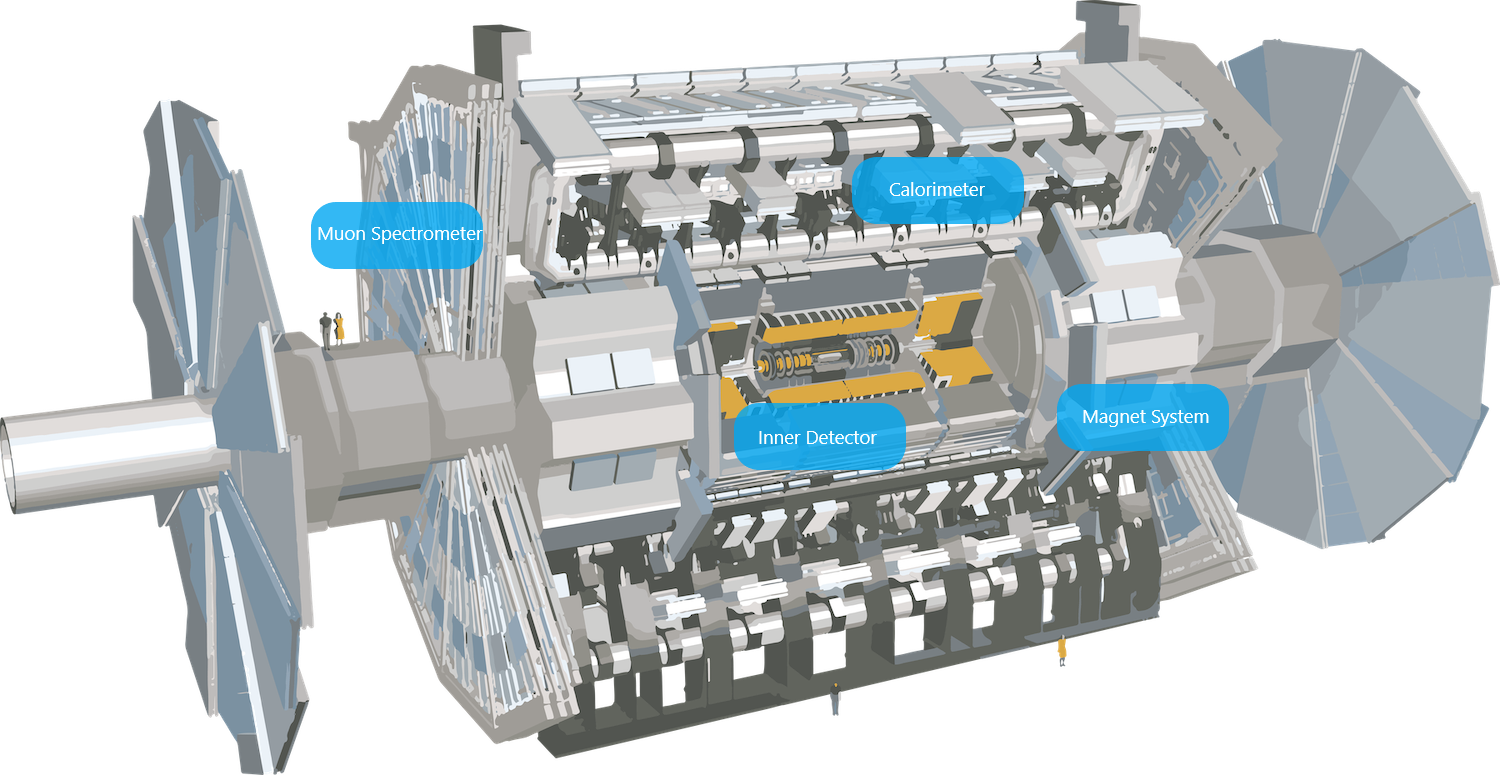
\includegraphics[width=10cm,height=7cm,keepaspectratio]{Figures/Intro/Detector reduce.png}
    \caption{The schematic view and length-wise cross-section of the ATLAS detector consisting of the Magnetic system, Inner detector, Calorimeter, and Muon Spectrometer, and showing the scale of the detector compared to a human. ATLAS Experiment  \copyright 2024 CERN}
    \label{fig:ATLASdetector}
\end{figure}

After each proton-proton collision energized by LHC inside the ATLAS detector, various processes take place to detect and analyze the produced particles and their interactions.\\
The first interaction of the produced particles with the detector takes place at the Inner Detector, positioned closest to the interaction point where proton-proton collisions occur. The currently installed and commissioning inner detector, consists of three components namely the Pixel Detector, Semiconductor Tracker (SCT), and Transition Radiation Tracker (TRT), is highly sensitive and rather smaller in size compared to the Calorimeters and Muon Spectrometer, and has a responsibility of the identification of electrons, photons, muons, and tau-leptons produced in both heavy-ion collisions and proton-proton interactions, as well as charged-particle reconstruction and heavy-flavour tagging. Additionally, it is used for reconstructing the trajectories of charged particles and is utilized in pile-up vertices and pile-up jet rejection, identification of primary and secondary vertices, complete reconstruction of exclusive decay modes, tracking of interactions and photon conversions, and particle identification through transition radiation and $dE/dx$. \\
The current ATLAS Inner Tracking Detector was designed to operate at a $14  \si{\tera\eV}$ center-of-mass energy, an average pile-up of $23$ proton-proton interactions per crossing\footnote{The term "proton-proton interaction per crossing" describes the number of interactions or collisions that take place between protons each time a proton beam crosses over another at a particle accelerator's collision site. Protons travel in opposing directions and collide at certain points of interaction when used in experiments at facilities like CERN's LHC. More @ \href{https://lhc-machine-outreach.web.cern.ch/collisions.htm}{LHC Machine outreach}}, and a constant instantaneous luminosity of $L = \num{1e34} \si{\square\per\centi\meter\per\second}$. Later in operation, it exceeded the average pile-up of $24.2$ and the peak instantaneous luminosity of $L = \num{1.37e34}. \si{\square\per\centi\meter\per\second}$\cite{Collaboration:390920}

%commented section about the other parts of the detector
\begin{comment}
    

The Calorimeter has the responsibility of measuring the energy of the particles. The calorimetry system in the ATLAS detector consists of the Liquid Argon (LAr) Calorimeter (Electromagnetic Calorimeter) and the Tile Hadronic Calorimeter (Fig.\ref{fig:detectorAppendix}). The particles interact, are absorbed, and finally converted into a shower of lower energy particles by the high-density material in the Electromagnetic calorimeters. As a result of this process, the 'new' particles ionize the liquid Argon producing an electric current that can be measured and the cumulative currents show the energy of the original particle. The Hadronic Calorimeter has a similar functionality, but due to its design which consists of several layers of steel and plastic scintillating tiles, interacts with the Hadronic particles, which do not deposit all of their energy in the LAr Calorimeter.\\
The outmost layer is where the Muon Spectrometer is placed. Muons are unique in their ability to penetrate dense materials, and they carry information about particles that might be missed by the inner layers of the detector. Muon Spectrometer consists of five different detector technologies: Thin Gap Chambers, Resistive Plate Chambers, Monitored Drift Tubes, Small-Strip Thin-Gap Chambers, and Micromegas, allowing us to spot and measure the momentum of muons (Fig.\ref{fig:detectorAppendix}).\\
Finally, the Magnetic System provides a magnetic field to precisely measure particle momenta. This feature helps for a better understanding of particle energies and collision dynamics (Fig.\ref{fig:detectorAppendix}). The Triggering System mainly selects interesting collision events and filters them from the enormous amount of data, managing the data inquisition and preventing it from overflowing. Together, these systems enhance the efficiency and precision of the ATLAS detector at the LHC.\cite{ATLASweb}\\
 A schematic view of the particle detection, shortly explained above, is shown in Fig.\ref{fig:ATLASlayers}.

\begin{figure}[h]
    \centering
    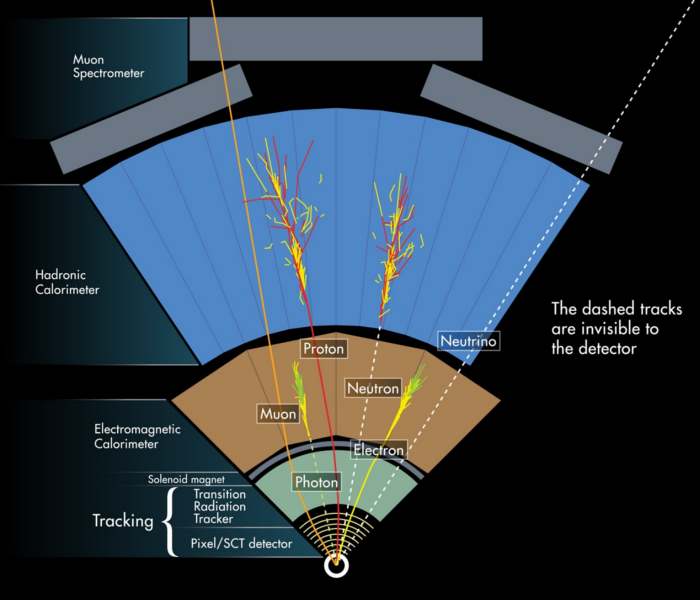
\includegraphics[width=10cm,height=10cm,keepaspectratio]{Figures/Intro/layers.png}
    \caption{An illustrated view of particle detection in the ATLAS detector, showcasing layers of different instruments. Inner detectors trace charged particle paths, calorimeters measure energy deposition, and muon detectors identify and track penetrating muons. This comprehensive system unveils the intricate details of high-energy particle interactions. \href{http://collider.physics.ox.ac.uk/}{Collider}\copyright University of Oxford, 2016 }
    \label{fig:ATLASlayers}
\end{figure}
\end{comment}

As the ongoing and anticipated discoveries within the project continually generate new questions, it drives us to further investigations and explore new areas. As a result, it becomes necessary to design and upgrade detectors. We ensure that we stay at the forefront of scientific investigation and meet the changing needs of our research by improving our detecting skills. The Inner Tracker upgrade gives us more accuracy and capacity to record the finer details of particle interactions. We can push the limits of our knowledge owing to this constant progress, which has helped us make important advancements in high-energy physics. The inner tracker is undergoing a major upgrade to make this goal possible. The goals of the ITk upgrade project include improving tracking precision, handling higher particle fluxes, and ensuring the detector's resilience in the challenging environment of the upgraded High-Luminosity LHC (HL-LHC), which will provide even more intense beams of protons. It is expected to achieve an average of $140$–$200$ inelastic proton-proton collisions per crossing, with the instantaneous luminosities of $L = 5-\num{7.5e34} \si{\square\per\centi\meter\per\second} $ at a $14  \si{\tera\eV}$ center-of-mass energy. This design promises a total data set of $4000 \si{\per\femtobarn}$ \footnote{"\textit{Integrated luminosity is usually expressed in units of “inverse femtobarns” ($\si{\per\femtobarn}$). A femtobarn is a unit of cross-section, a measure of the probability for a process to occur in a particle interaction. This is best illustrated with an example: the total cross-section for Higgs boson production in proton–proton collisions at $13 \si{\tera\eV}$ at the LHC is of the order of $6000\si{\per\femtobarn}$. This means that every time the LHC delivers $1\si{\per\femtobarn}$$ of integrated luminosity, about $6000 \si{\per\femtobarn}$ x 1 $\si{\femtobarn} = $6000$ Higgs bosons are produced.}"\cite{CERNweb}} over the $10$ years of prospective operation time of the new ATLAS ITk detector. \\

The new detector consists of multiple layers of silicon particle detectors; Silicon microstrip sensors will make up the outermost layers, with four concentric barrel layers and one end-cap section featuring six disks on each barrel side, while silicon pixel sensors will form the innermost layers. The Long Strip modules (LS modules) with $48.35 \si{\milli\meter}$ strips length are placed in the outer two barrel layers, while the Short Strip modules (SS modules) with parallel strips length of $24.16 \si{\milli\meter}$ length are housed in the inner two barrel layers. Six disks per side, with trapezoidal-shaped sensors of varying lengths and strip pitches, make up the forward portions of the end-cap strip tracker.  This new design is expected to endure the extremely harsh radiation environment, which the current inner detector is vulnerable to at Pixel detector, Semiconductor Tracker (SCT), and Transition Radiation Tracker (TRT), by substituting the electronic parts of the older design with hybrid silicon pixels, providing $3$ times more silicon area of the current ID, and lowering the risk of the damaging the sensor due to the high radiation.\cite{herde2023atlas}. Figure \ref{fig:ITklayout} shows the schematic view of the layout of the Inner Tracker and the main detector's components.\\

\begin{figure*}[h]
    \centering
    \begin{subfigure}[t]{0.45\textwidth}
        \centering
        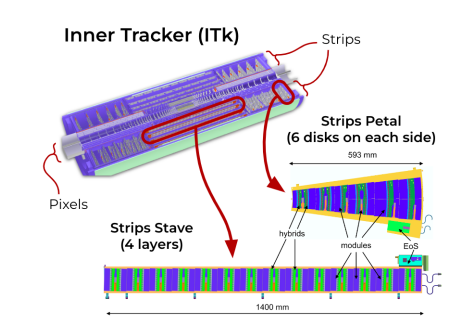
\includegraphics[height=4.5cm]{Figures/Intro/component.PNG}
        \caption{} \label{fig:ITklayout1}
    \end{subfigure}
    ~ 
    \begin{subfigure}[t]{0.45\textwidth}
        \centering
        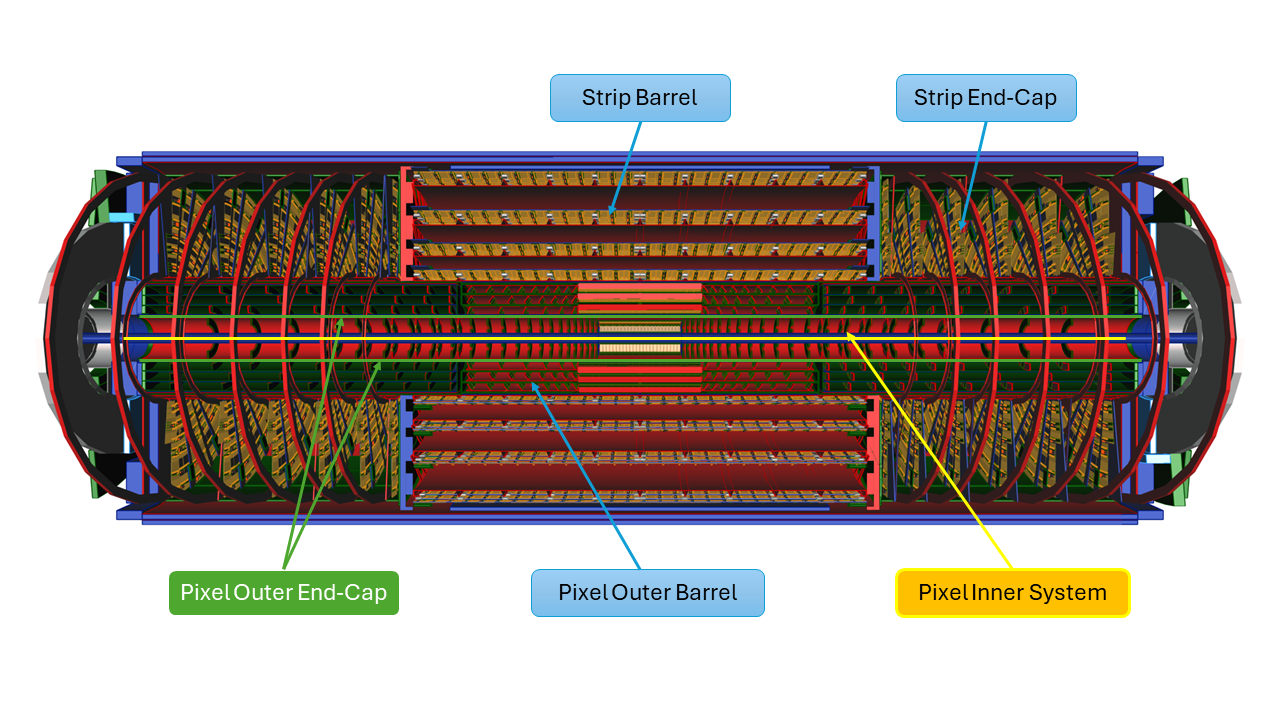
\includegraphics[height=4cm]{Figures/Intro/fig_07Edited.png}
        \caption{}
        \label{fig:ITklayout2}
    \end{subfigure}
    \caption{a) A schematic view of ITk showing the pixel detector surrounded by a Strip Detector Picture from \cite{itkcomponent}, and b) Cross-section view of the Inner Tracker showcasing the Strip barrel, Strip end-cap, Pixel outer end-cap, Pixel outer barrel, and Pixel inner system. Picture from \cite{ATL-PHYS-PUB-2021-024}} 
    \label{fig:ITklayout}
\end{figure*}





As the precision and consistency of the acquired data are directly dependent on these modules, it is crucial to perform various rigorous tests to spot any potential glitches or deviations in performance that might compromise the integrity of experimental outcomes. With ATLAS ITk modules serving as the primary data collectors in the critical particle collision environment at the LHC, reliability testing of these components is essential, to ensure that each module operates at peak efficiency, minimizing data inaccuracies and strengthening the reliability of scientific findings.\\
Since the scope of the upgrade project is very big and beyond any single institute to cover all aspects of the project, it requires close collaboration between multiple research institutions, laboratories, and experts in various fields, and the testing part of the ITk module production indeed requires the collaboration of several scientific institutes. However, the information and the data stream related to each part of the test have to be consistent and cover all the required data for further analysis and probing. This thesis focuses on the reliability testing of ATLAS ITk modules, and its primary goal is to conduct thorough and rigorous tests to identify potential vulnerabilities, weaknesses, or variations in performance by tracking the performance in different environmental and experimental situations, the stability of the components and data handling, and quality control of the modules specifically for the long-term usage. The project mainly consists of $4$ different parts: 
%edit this better
\begin{itemize}
    \item an attempt to add additional information to the test data
    \item establishing a connection to the database to store the data for further analysis proficiently
    \item setting up a test environment and performing the long-term reliability tests
    \item analyzing the data gathered by the tests
\end{itemize}

Given that there is no turning back once the modules are installed, it emphasizes the importance of carrying out extensive long-term reliability testing. Identifying their optimal functionality and dependency is crucial, as any doubts or problems that arise after installation would be permanent. This proactive approach reduces the possibility of unanticipated issues and gives stakeholders confidence that the modules will function seamlessly and dependably in their assigned roles.\\

Subsequently, readers can expect to delve into a comprehensive exploration of the mentioned topic, beginning with an introduction to the test setup, including the configuration and instrumentation utilized to conduct the tests. Additionally, we will outline the different executable controlling systems of the tests, as well as methods of storing and merging the data gathered from the data for further analysis. Lastly, we present the results from the long-term reliability test of the modules, perform a comprehensive analysis of the test data, and preview the validity of the quality of the manufactured modules. 
%write a bit about this text being a reference for text
%add a bit more on HL-LHC and less about modules. 
%Add itk layout: layout of pixel and strips
% Modules

\chapter{Modules} % Main chapter title

\label{Modules} % For referencing the chapter elsewhere, use \ref{Results} 

%----------------------------------------------------------------------------------------

% Define some commands to keep the formatting separated from the content 
\newcommand{\keyword}[1]{\textbf{#1}}
\newcommand{\tabhead}[1]{\textbf{#1}}
\newcommand{\code}[1]{\texttt{#1}}
\newcommand{\file}[1]{\texttt{\bfseries#1}}
\newcommand{\option}[1]{\texttt{\itshape#1}}

%----------------------------------------------------------------------------------------
\section{ITk Strip Module Design }
A ITK strip module\protect\footnote{For the scope of this thesis, while certain aspects of the barrel modules have been addressed, the primary emphasis will be directed toward the end-cap modules.} consists of $3$ main parts: sensor, hybrid, and power board.
The foundation of the ITk Strip module is made of a $300 \si{\micro\meter}$ thick silicon sensor. The hybrids including Kapton PCBs, read-out chips, and control chips, and a power control board which powers the whole module, are installed on the top of the sensor. Fig.\ref{fig:modulelayout} shows an illustrated view of the ATLAS ITk module, showcasing the silicon sensor, hybrid, and power boards, with their different components.\\

\begin{wrapfigure}{R}{7cm}
    \centering
    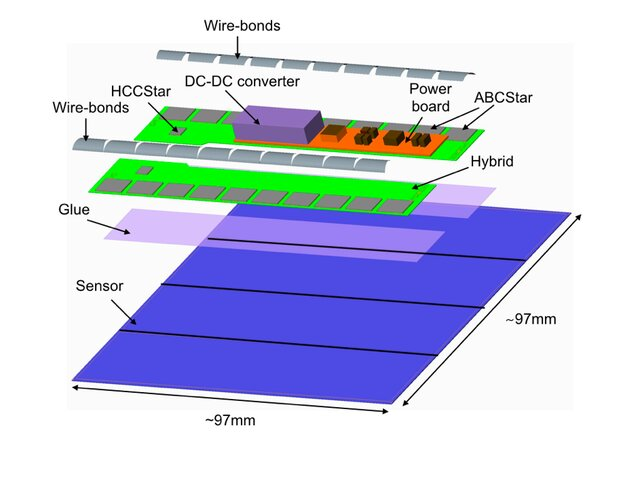
\includegraphics[width=7cm,height=10cm,keepaspectratio]{Figures/modules/modulelayout.jpg}
    \caption{An overview of an ITk module structure consisting of the silicon sensor, hybrid, and powerboard \cite{Collaboration:390920}.}
    \label{fig:modulelayout}
\end{wrapfigure}

\subsection{n$^+$-in-p silicon sensor}
The strip module is made of silicon, a semiconductor material that is sensitive to the presence of electric charge. The strip consists of a series of thin silicon strips arranged in a grid-like pattern. Each strip acts as an individual sensor capable of detecting the passage of charged particles and is made from silicon semiconductor material that has been doped with impurities to create specific types of charge carriers: p-type Silicon and n-type Silicon. In p-type material, atoms are doped with impurities that have one fewer electron in their outer shell than silicon. This creates "holes" or positively charged charge carriers where electrons are missing. On the other hand, in n-type material, atoms are doped with which have one extra electron in their outer shell compared to silicon. This results in an excess of negative charge carriers or free electrons.\\
When p-type and n-type silicon regions come into contact, a depletion region forms due to diffusion and electrostatic forces. In this area, free carriers (electrons in n-type and holes in p-type) combine, leaving behind charged ions. This causes a region with no charge carriers, making it insulating. A bias voltage is applied across the p-n junction, in a reverse bias configuration for silicon strip detectors. This reverse bias voltage widens the depletion region, improving the insulating properties. An illustration of a typical p-n junction is shown in Fig.\ref{fig:siliconpnjunction}.\\

\begin{figure}[h]
    \begin{subfigure}[b]{0.45\textwidth}
        \centering
        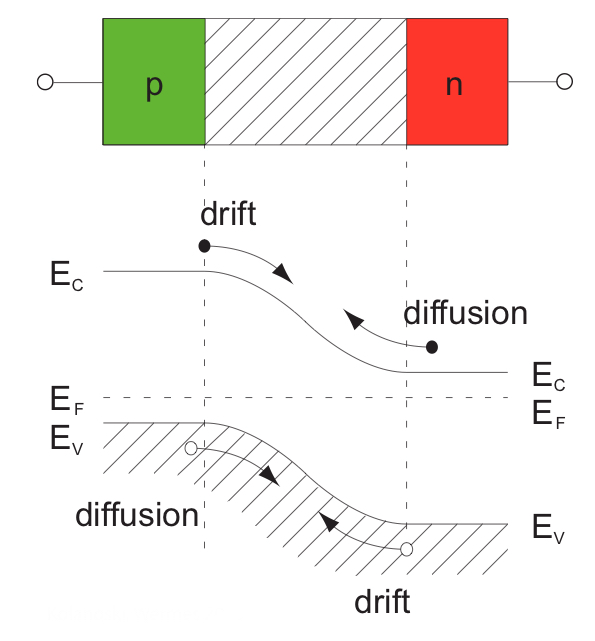
\includegraphics[width=6.5cm,height=10cm,keepaspectratio]{Figures/modules/Pnjunction.png}
        \caption{}\label{fig:siliconpnjunction}
    \end{subfigure}
    ~
    \begin{subfigure}[b]{0.45\textwidth}
        \centering
        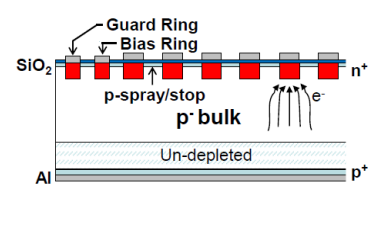
\includegraphics[width=6.5cm,height=10cm,keepaspectratio]{Figures/modules/striplayout.PNG}
        \caption{}\label{fig:striplayout}
    \end{subfigure}
    \caption{a) A schematic of a pn junction demonstrating the Fermi energy level ($E_f$), electron and hole movement, and the physical interaction within the semiconductor material\cite{kolanski}, and b) A schematic view of the n$^+$-in-p strip device\cite{striplayout}}
    
\end{figure}

When a charged particle passes through the silicon strip detector, it interacts with the silicon atoms, ionizing the particles interacting along its path. This ionization results in the creation of electron-hole pairs within the semiconductor material. The silicon strip detector is designed with a built-in electric field, which causes the newly created charges (electrons and holes) to move in opposite directions toward the positively and negatively biased electrodes, respectively. As the electrons and holes move toward the electrodes, they create an electric current in the silicon strips with a magnitude proportional to the energy deposited by the passing particle. The electric signals generated by the passage of particles through the silicon strips are amplified, digitized, and recorded by the detector's readout electronics. These signals are then analyzed by customized algorithms to reconstruct the trajectories of the charged particles and deduce their properties such as momentum, charge, and energy.\\

However, the biggest difference between the previous generation of the inner detector and the newly arrived ITk is the use of n$^+$-in-p strips. In this structure, the silicon bulk (the main body of the detector) is p-type. Near the surface of the silicon, there is a thin layer of heavily doped n-type material (n$^+$), which contains excess electrons as majority carriers. This creates a built-in electric field that facilitates the collection of charge carriers generated by particle interactions, which allows this configuration to acquire superior charge collection compared to the n-in-p configuration.\\

These strips can tolerate high levels of radiation and operate at voltages up to $700 \si{\volt}$. These properties give the advantage to the ITk module over the current ATLAS SCT modules to show exceptionally better signal performance after irradiation. n$^+$-in-p sensors deliver approximately twice as much charge compared to p-in-n sensors. Additionally, n$^+$-in-p technology is preferred due to lower costs, higher availability of foundries, and comparable signal sizes to n+-in-n sensors\cite{UNNO2013183}.\\

The silicon strip sensor as the sensing elements, which also are referred to as "Channels" when connected to the readout chips, are responsible for detecting and measuring the signals produced by charged particles. In ITK modules, channels are arranged in the form of very thin wafers of strips along the surface of the sensor. Each strip acts as an individual sensing element and is connected to readout electronics at one end. The number of channels in a strip sensor of ITk modules varies between each module due to the difference in geometry and the number of read-out chips.\\

%micrsocope picture

\subsection{Hybrid}
Hybrids act as a bridge between the readout electronics and the silicon sensor, enabling the conversion of sensor signals into digital data that can be handled and examined. These hybrids are designed to provide a platform for mounting and connecting the ABCStar readout chips, which are responsible for amplification, shaping, and digitizing the signals produced by particle interactions in the silicon sensor, and HCCstar which facilitates communication between the readout chips and the external control systems. \textcolor{blue}{By design, each hybrid is mounted on one side of the module, sitting directly on one of the sensors and bounded to both sensors separately. The part that the hybrid is mounted on is referred to as "Under", and the second part is referred to as "Away". The connection between the silicon stripes and the readout chips on the hybrids are made by $2$ thin wire threads, each connected to one side of the silicon strip (n and p)}  \\

%micrsocope picture

\subsection{Power board}
The front-end electronics of the hybrids get low voltage (LV) power from the power board via a DC-DC converter, which increases the voltage to the required levels. To ensure that the silicon sensor runs at the ideal voltage for signal detection, the power component also enables sensor high voltage (HV) biasing\cite{sykora2019itk} (high voltage creates an electric field within the sensor, which helps to accelerate and collect charge carriers (electrons and holes) generated by particle interactions). \cite{Collaboration:390920}. \\
In the heart of the power board, an Autonomous Monitoring And Control (AMAC) chip is installed in order to monitor and control the input and output electrical information of the module components. AMAC continuously monitors important parameters of the ITk module, such as voltage, and current, and if a parameter exceeds safe limits, it can take corrective actions. This might involve adjusting voltages or even shutting down the module to prevent damage.

\section{ITk Detector Design}
The new ATLAS ITk is an all-silicon detector, consisting of two major sub-systems of Pixel detector (ITk-Pixel) which will be placed closest to the beamline, and Strip detector (ITk-Strip) which would cover the bigger outer area. The strip detector itself, breaks down into two main subcategories of silicon strip modules, to cover the maximum area around the collision point: Barrel modules and End-cap modules.

\subsection{Barrel modules}
The beamline is encircled by four $2.8 \si{\meter}$-long cylinders, each consisting of $392$ staves consisting of $28$ modules on each (both sides, $14$ modules each), that make up the strip barrel. Two lengths of strips are used for the barrel: Long Strips (LS) with the length of $48.2  \si{\milli\meter}$ perform effectively in the lower occupancy zone at greater radii (layers L2 and L3), while Short Strips (SS) with the length of $24.1  \si{\milli\meter}$ are required for further subdivision at lower radii (layers L0 and L1). The main reason for this deviation in lengths is hidden in their final installation position around the beam. SS modules are located closer to the collision points and are expected to receive more flux from the collisions. To handle the higher flux of data, these modules have two dedicated hybrids with $10$ readout chips installed on each, which increases the processing power of each module consequently. On the other hand, LS modules are equipped with one hybrid and $10$ read-out chips and are located on the farther barrels from the beamline. 

\subsection{End-cap modules}
To give the best coverage, the strip end-caps (designated as end-cap A and end-cap C) feature six disks on each side.\\
 
The end-caps consist of $32$ identical "petals" on each disk. These petals are designed to cover the circular area of the barrel ends, and each hosts a total of $9$ modules with $6$ different geometries (R0 to R5). The sensors in the end-cap have two curving edges that form concentric arcs of circles centered at the disk's center (center of the beam), giving them an approximately trapezoidal shape. The difference in the geometry of the modules leads also to different strip lengths and different numbers of hybrids and read-out chips in each class. This difference is also important for the testing procedure because each module must be introduced separately due to its class to the testing environment to receive its own configuration for the test. 
Fig.\ref{fig:picModules} shows pictures of the LS and SS for the barrel, and R0 to R5 modules for the end-cap. (Higher resolution picture is shown in Fig.\ref{fig:picModules-large}). Also, Table.\ref{tab:moduleLaout} is listing the details of each module. 

\begin{figure}[h]
    \begin{subfigure}[b]{0.45\textwidth}
        \centering
        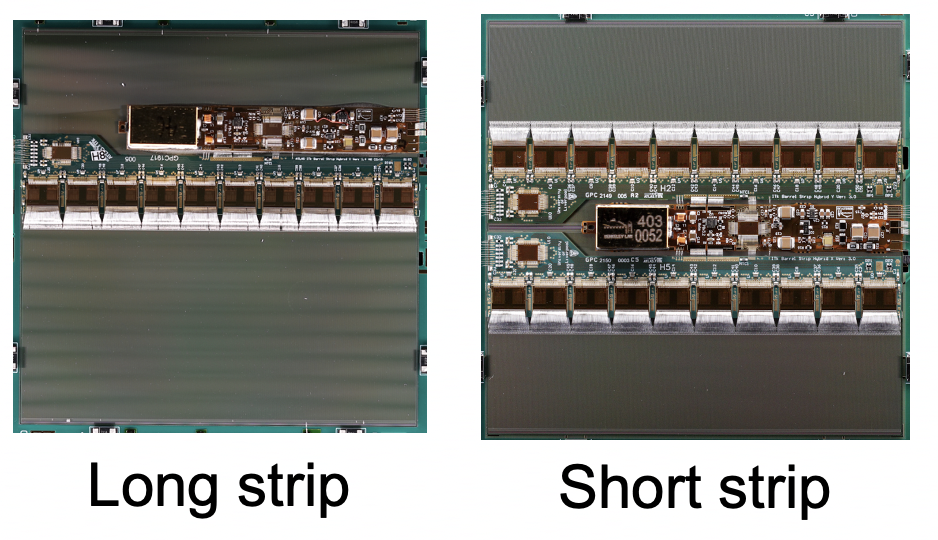
\includegraphics[width=7cm,height=15cm,keepaspectratio]{Figures/modules/Barrel_Modules.png}
        \caption{}\label{fig:barrel}
    \end{subfigure}
    \begin{subfigure}[b]{0.45\textwidth}
        \centering
        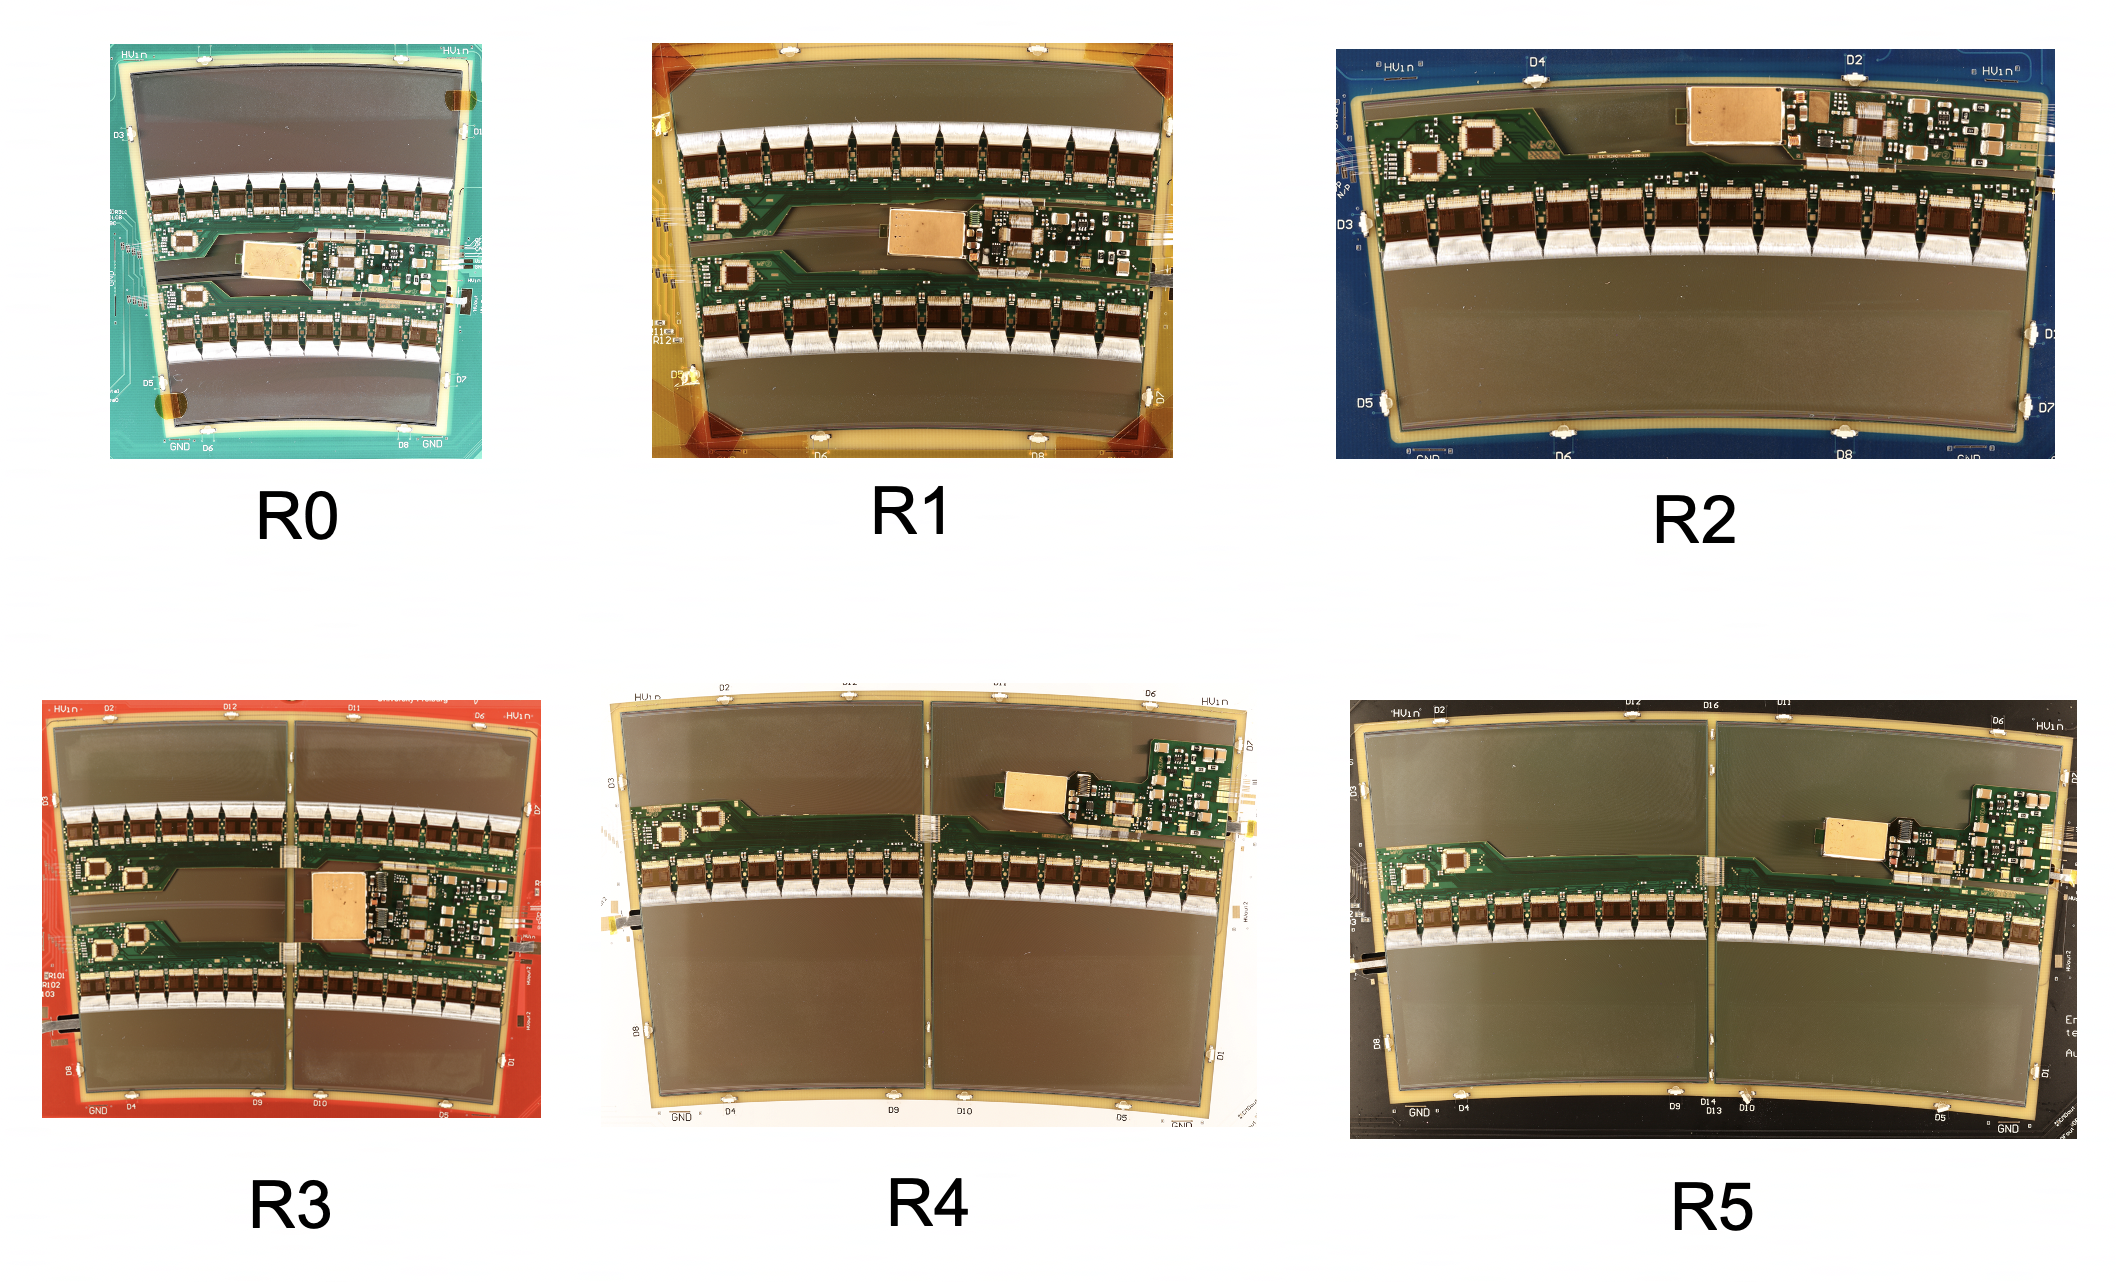
\includegraphics[width=7cm,height=15cm,keepaspectratio]{Figures/modules/EC_Modules.png}
        \caption{}\label{fig:endcap}
    \end{subfigure}
        \caption{Top view pictures of a) barrel modules including LS and SS, and b) end-cap modules including R0 to R5\cite{tishelman2024quality} }
        \label{fig:picModules}
\end{figure}

In total, an area of $165.25 \si{\meter\squared}$, ($104.86 \si{\meter\squared}$ for barrel area, $60.4 \si{\meter\squared}$ for end-caps), is covered by $17888$ modules in the new ITk detector. This area gives the coverage of $10^{\circ}$ of the beam axis, or $\pm 2.7$ units of pseudo rapidity to the strip system. Some additional overviews of the detector and modules' layout are shown in Fig.\ref{fig:additionalLayout}\cite{Collaboration:390920}. 



% Test

\chapter{Test and Test setup} % Main chapter title

\label{Test} % For referencing the chapter elsewhere, use \ref{method} 

%----------------------------------------------------------------------------------------
The Long Term Reliability Testing (LTRT) of ATLAS ITk modules is intended to be conducted through a systematic approach aimed at evaluating their performance under various conditions. In this section, we will introduce the test setup and the test software and controls in detail, and outline and provide an explanation of each test performed during a full cold LTRT.\\

\section{Test Setup}

The test setup designed for thermal cycling and long-term reliability testing is specialized equipment that can maintain an environment with temperature and humidity controlled for testing the performance of detector components. \textcolor{blue}{In addition to that, it provides an isolated environment to prevent unwanted photons and electromagnetic noises disturb the test.} This equipment, known as "Coldbox", typically have the capability to reach and maintain a range of low temperatures. This temperature range is chosen to simulate the operating conditions of the detector, which is chosen because the noise is significantly reduced at this temperature. In addition to the temperature, Coldbox regulates and monitors several environmental parameters such as relative humidity, airflow, and dew point, and is also able to control temperature for each installed module. Fig.\ref{fig:coldbox} shows an overview of the equipment. \\

\begin{figure}[h]
    
    \begin{subfigure}[b]{0.45\textwidth}
        \centering
        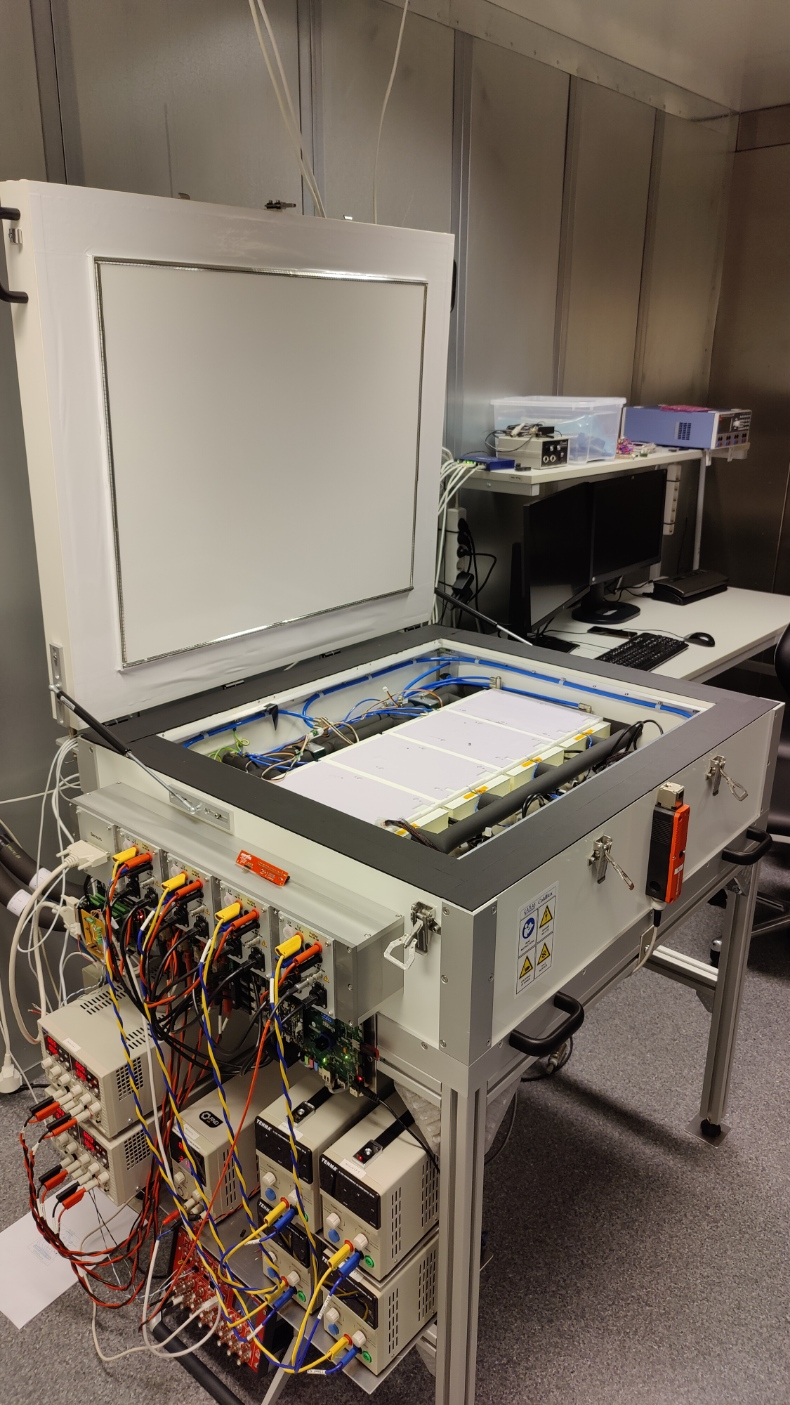
\includegraphics[width=7cm,height=8cm,keepaspectratio]{Figures/test/coldbox-1.jpg}
        \caption{}\label{fig:coldbox1}
    \end{subfigure}
    ~
    \begin{subfigure}[b]{0.45\textwidth}
        \centering
        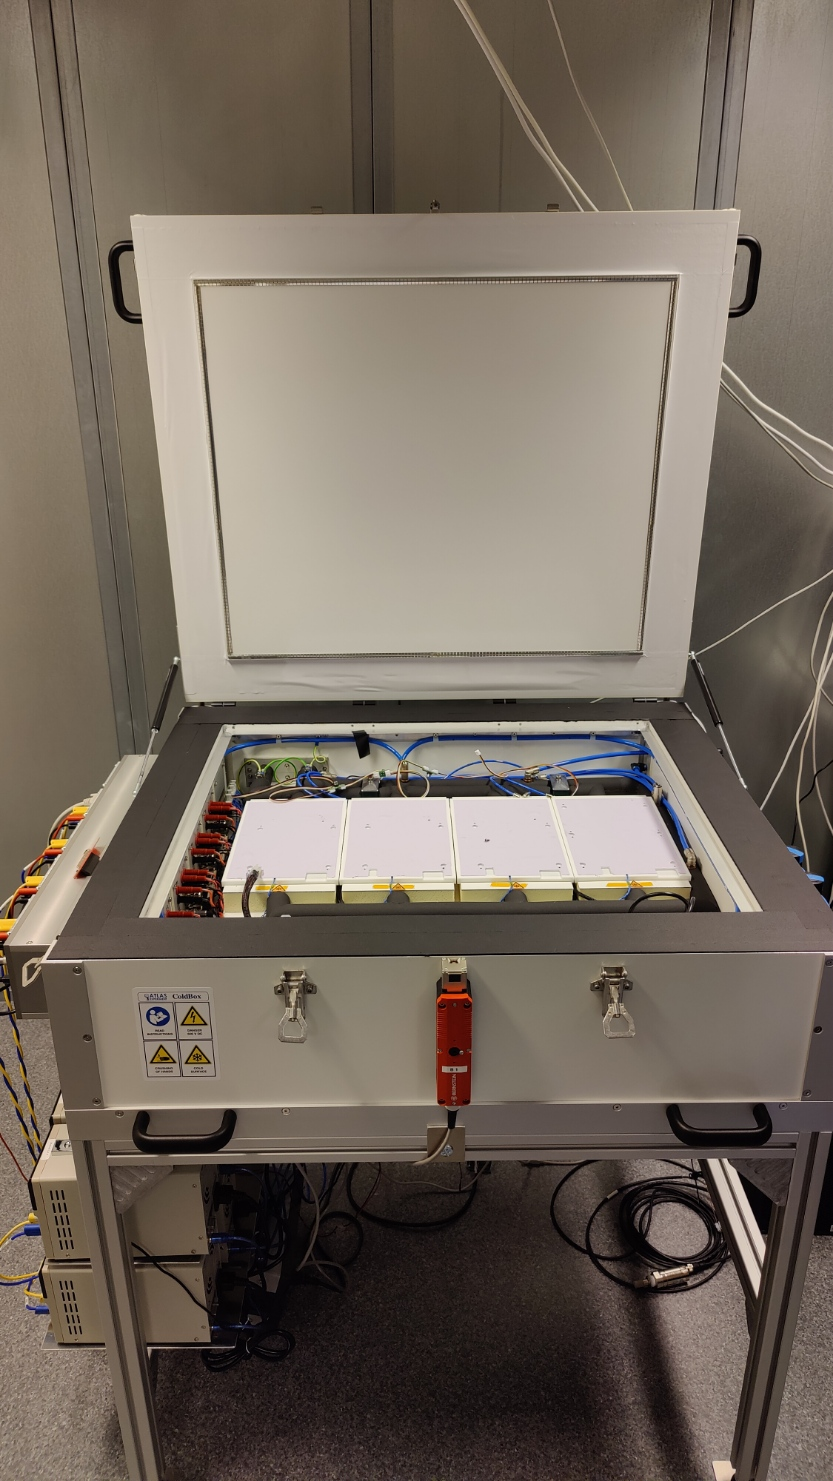
\includegraphics[width=7cm,height=8cm,keepaspectratio]{Figures/test/coldbox-2.jpg}
        \caption{}\label{fig:coldbox2}
    \end{subfigure}
    \caption{An overview of the Coldbox from a) front view, and b) side view, showcasing the general properties of the equipment and connected devices and sensors.}
    \label{fig:coldbox}
\end{figure}

\subsection{Coldbox}
The long-term reliability testing is conducted under a regulated setting with a fixed temperature of $-35\si{\celsius}$, \textcolor{blue}{but for the proof of concept intended for this work, and reduce the temperature regulation time, the tests are conducted at $0\si{\celsius}$.} The environmental parameters are monitored and maintained constant by the Coldbox throughout the duration of the test (Active and IDLE). The temperature of each module is controlled zonally by $4$ "chucks", on which one module can be installed. Heat sinks attached to a chiller and "Peltier" components are positioned on each chuck to allow the temperature of the modules to be precisely changed and set on demand.\\

Coldbox is equipped with four different types of power supplies: $4$ individual Low Voltage (LV) power supplies, responsible for powering each installed module, a High Voltage (HV) power supply, to inject the test charge to the modules, $4$ individual power supplies to heat up the Peltiers separately (Fig.\ref{fig:supplies}), and one power supply to power the airflow system, RaspberryPi board, interlock, and by-pass valves. The operating voltage of the modules is typically $\approx 11 \si{\volt}$. The HV power supply, on the other hand, delivers up to $500 \si{\volt}$ for the purpose of these tests (bias of $-500 \si{\volt}$). The operating voltage of the Peltiers' power supplies varies by the set temperature.\\

The box is cooled down to $30\si{\celsius}$ by an external chiller, using silicone oil as the coolant, and maintains the temperature of the Coldbox at a desired level during the tests. \textcolor{blue}{The exact desired temperature then is set by the Peltiers, which can increase or decrease the temperature of the module with great precision (Fig.\ref{fig:cooling}). The reason for this configuration is that first, as mentioned, the chiller cannot regulate the temperature årecicely as needed during the test, and second, pushing the peltiers to achieve to low temperature requires a great amount of current provided in a short time, which will cause serious issue to them.}\\
In addition to the above, the airflow is controlled \textcolor{red}{WHY?} and maintained using a flow control valve and a digital flow meter (Fig.\ref{fig:airflow1} to \ref{fig:airflow3}). \\

Outside the box, 3 different controller boards are installed; a RaspberryPi board running coldjiglib which is the commanding unit of the Coldbox, \textcolor{blue}{a polarity switch that is responsible for alternating the current of the Peltiers}, and a data collection unit that holds 4(+1) data ports, each for one module (Fig.\ref{fig:connections})\\

The relative humidity on each module is measured using a humidity sensor. These sensors are installed at the end of the outlet flow connection, and read the humidity of the flown air inside the installed module's casing. Using the relative humidity and the temperature of the air on each module, we can calculate the dew point using Eq.\ref{eq:dewpoint}. \textcolor{blue}{These measurements, and the dew point value, in particular, are crucial to preventing the formation of water droplets on the electronic components.}\\

\textcolor{blue}{Lastly, the box is secured and locked by an interlock system, to implement safety measurements due to the high voltage presence during the tests}, as well as to prevent unwanted access to the box during the tests and exposure of the modules to the ambient environment. \footnote{for more information please refer to \textcolor{red}{EDU's Thesis}.} (Fig.\ref{fig:interlock}).\\


\subsection{Test Software and Controls}
The configuration of the modules, calibrations, tests, and data collection from the tests are handled by the ITk Strip Data Acquisition (ITSDAQ) software developed by the strip community. After installation of the modules, each module depending on the type needed to be introduced to ITSDAQ in order to get the correct module configurations. Each LTRT test starts with a "Pre-Test" procedure, which acquires an IV test before powering on the hybrid (\textbf{WHY??}), and then, the hybrid is powered and the cooldown procedure is initiated. \textcolor{blue}{As the ColdBox regulates the environmental parameters, and it reaches to the desired cold temperature}, the high voltage is injected, and subsequently, the ABCstar full test is run. This procedure is repeated between pre-set intervals (typically every 12 hours for LTRT, \textcolor{blue}{but for the purpose of this work in very short intervals of 10 to 15 minutes}), for a required number of instances. \\

\textcolor{blue}{To ensure traceability during HL-LHC operation and subsequent stages of manufacture, it is imperative to record and preserve data from the QA/QC of each individual module. As more testing facilities are assigned for conducting LTRT and thermal cycling tests, it's critical to store test results in an international database for future analysis. In addition to the test results provided by ITSDAQ, and in order to validate the stability of the Coldbox and track down any potential abnormality in the test results of the modules, it is crucial to record and monitor the environmental and electrical data during the tests.} \\

\textcolor{blue}{Along with the above-mentioned considerations, another issue that needed to be taken into account was keeping these records safe and keeping them in a central database for upcoming research and studies. To address this problem and work with other testing facilities, we store all of the environmental, AMAC, and electrical test data along with the related metadata in different datasets. We then use the process that has been put into place to upload the data to a central database.}\footnote{\textcolor{blue}{The implemented procedure also captures the electrical data from the power supplies during normal operation, but during the development stage, this data is not returned by the software.}} Fig.\ref{fig:testworkflow} shows an overview of the workflow between different components of the test and the pathway of each relevant data to the database. 

\begin{figure}[h]
    \centering
    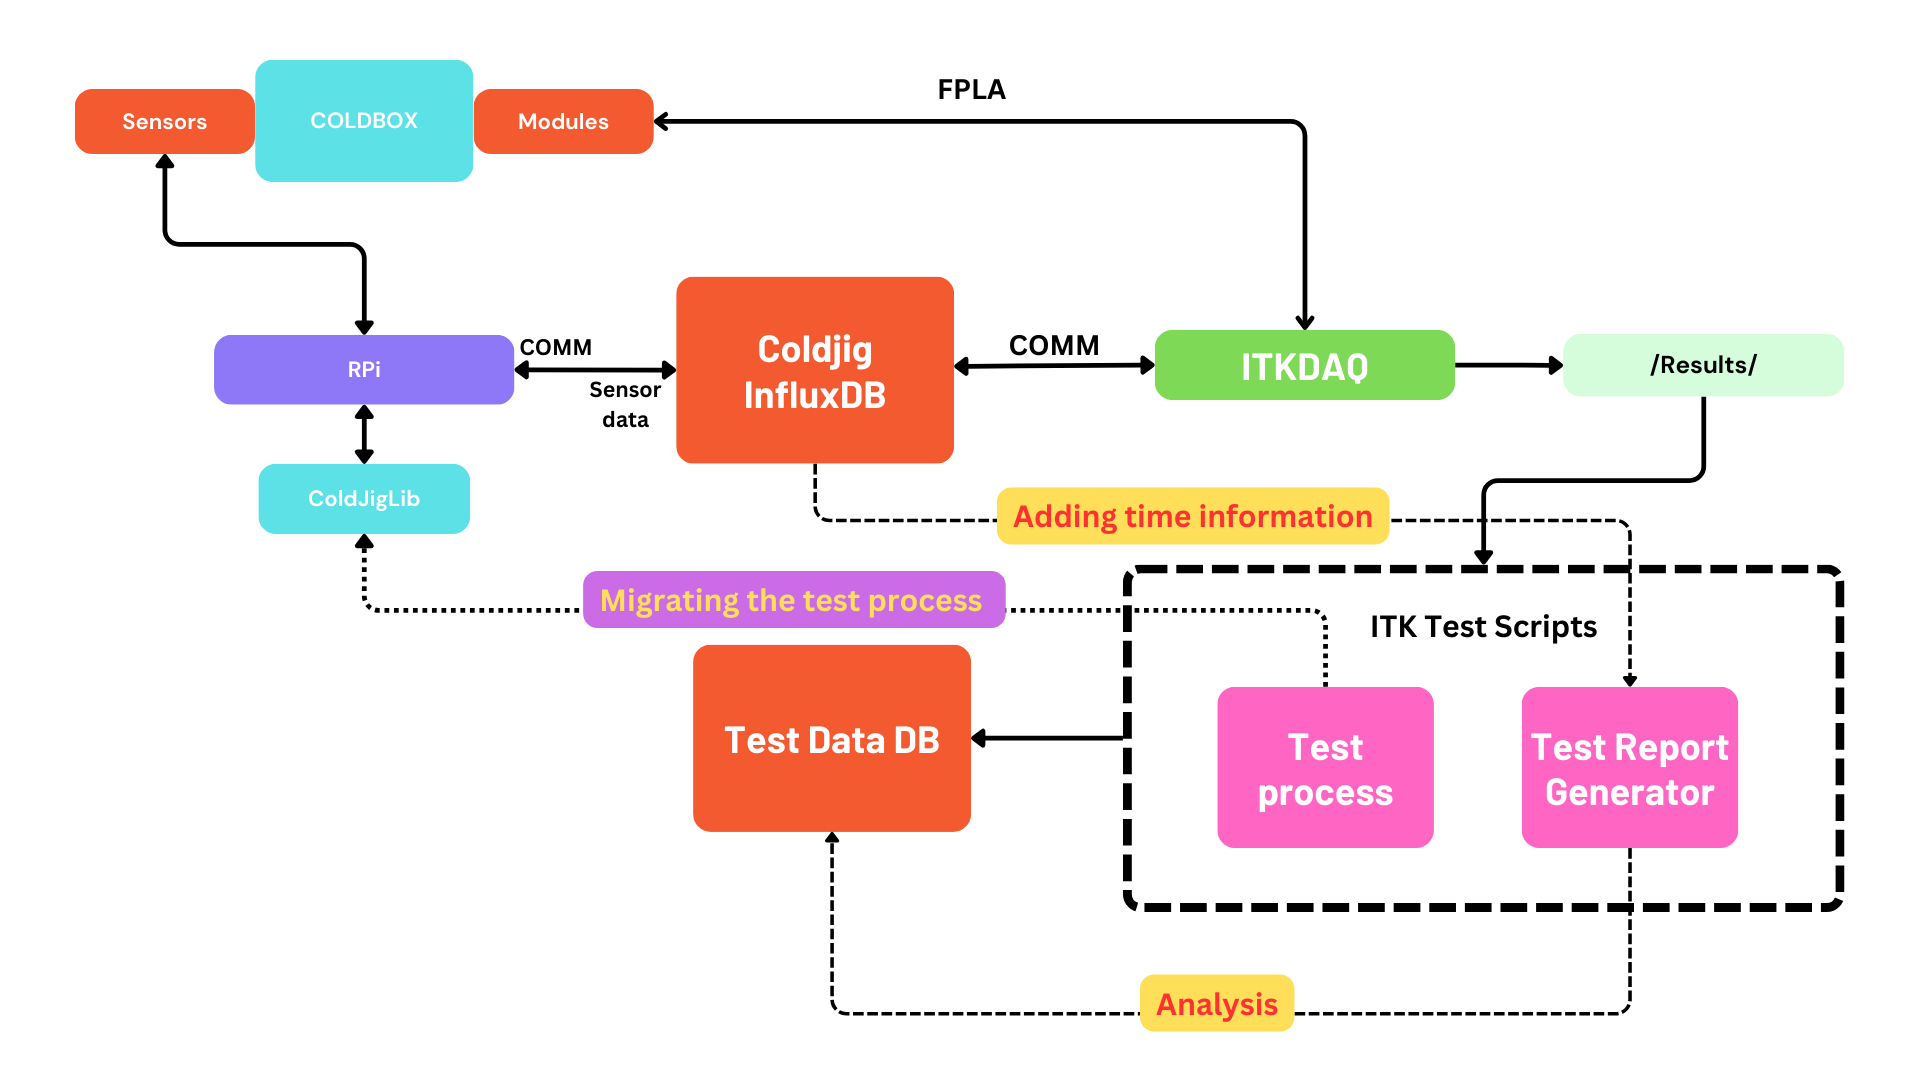
\includegraphics[width=10cm,height=11cm,keepaspectratio]{Figures/test/test diagram2.png}
    \caption{A diagram of the workflow of the LTRT test, from the start of the test}
    \label{fig:testworkflow}
\end{figure}

\subsection{The Environmental Data}
While ITSDAQ is essential for gathering and processing data from the ATLAS ITk modules, environmental data collection is not included in its scope. However, the integration of environmental data is crucial for a complete analysis and understanding of the modules' functionality. Temperature, dew points, relative humidity, and other variables can have a big impact on the behavior and dependability of modules. To accommodate these parameters, it is needed to retrieve data directly from the ColdBox and integrate it with the analyzed data from ITSDAQ. The ColdJiglib as the running heart of the Coldbox, enables us to gather environmental data. \\

As explained in the previous part, several LTRT tests are performed within a set time interval. Each test is tagged by the number of iterations and is presented by InfluxDB. To get access to the environmental data, we implemented a series of logics and queries, which find the latest test performed by presenting the test file, and find the time intervals in which the module was kept in the controlled environment (IDLE state) and the time interval that the LTRT is performed. The data is then stored in datasets with related metadata in order to be uploaded to the test database. \textcolor{blue}{ Afterwards, and for analytical purposes, we can compare the timestamps given by the environmental data and the test results, and we can examine the behavior of the module during the test in conjunction with the environmental data.}


\subsection{The Electrical Data}
In addition to the environmental data from the Coldbox, electrical data from the AMAC and the HV power supply needs to be monitored.\textcolor{blue}{ The AMAC data offers insightful information on how well the detector system is operating. Through the process of monitoring voltage levels, current consumption, and temperature, we are able to evaluate the general condition and operation of the detector components. It is important to mention that the AMAC individually records separate measurements of the temperature on each hybrid and the power board, as well as the voltage, current, and calibration parameters. Table \ref{tab:AMAC_params} enlisted the details of the measurement and parameters from AMAC.} 


\subsection{Physics behind the tests}
The tests (as we will be explained elaborately) are designed to characterize the electrical properties and performance of the ITk modules, particularly to determine the qualitative performance and endurance of the modules during the commissioning time. Several physical concepts are involved within the tests, that need to be explained before digging deep into the tests and their results. 

\subsubsection{Occupancy}
In the context of silicon detectors, occupancy refers to the fraction of detector elements that register a particle interaction within a specific time frame. It's essentially a measure of how "busy" the detector is. A high occupancy rate indicates a high level of particle activity or radiation in the detector, which can affect its ability to accurately measure particle tracks, identify particles, and distinguish between signal and background. Fig.\ref{fig:occupancy} illustrates the detection of particles in high and low occupancy situations.


\begin{figure}[h]
    \centering
    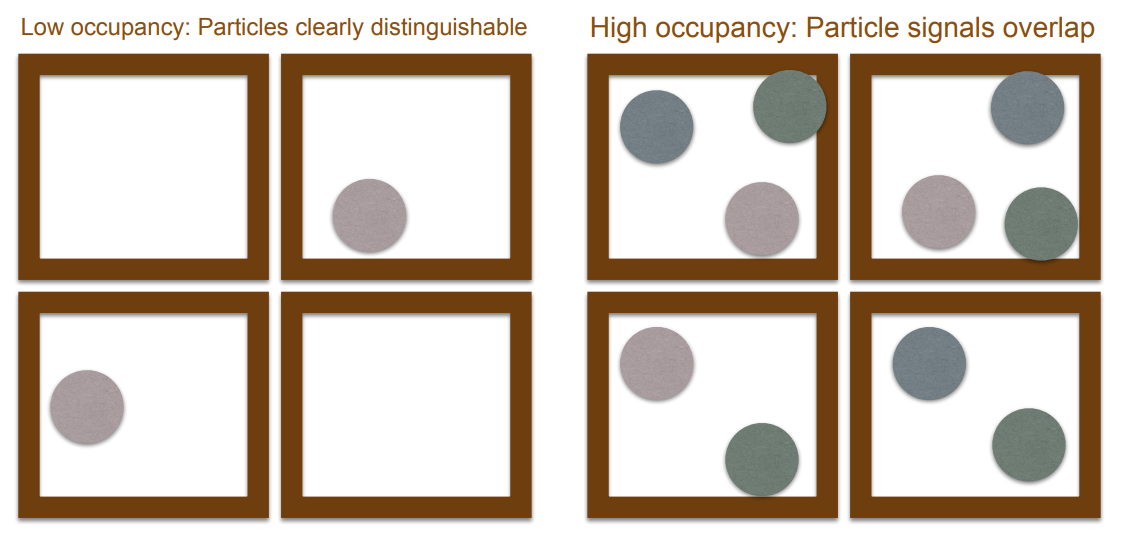
\includegraphics[width=8cm,height=7cm,keepaspectratio]{Figures/modules/occupancy.PNG}
    \caption{The schematic view of the detection of the particles by the silicon detector with a) low occupancy (left), and b) high occupancy(right)\cite{materClassDetection}.}
    \label{fig:occupancy}
\end{figure}

\subsubsection{Gain}
As explained in the previous part, the particles moving across silicon strips produce electric signals that are amplified and digitized, in order to be read-out. The process where the detector amplifies the signal generated by a particle interaction is referred to as gain. 
Due to the intrinsic voltage differential across the junction, when a particle interacts near it, the electric field accelerates the generated charge carriers across the junction, resulting in the creation of an extra current component. The overall signal may be improved by this additional current \cite{barr}.


\subsubsection{Threshold (Voltage threshold)}
\begin{wrapfigure}{r}{7cm}
    \centering
    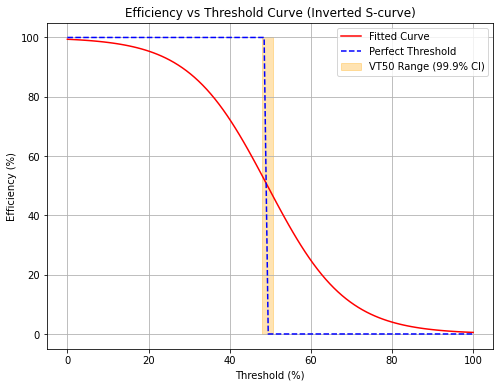
\includegraphics[width=7cm,height=7cm,keepaspectratio]{Figures/modules/threshold.png}
    \caption{A demo plot of the efficiency of the detection versus the threshold voltage (percentage from minimum to maximum operation voltage) showcasing the fitted curve and a perfect threshold.}
    \label{fig:threshold}
\end{wrapfigure}
The lowest voltage level required for generating a response or detection from the sensor or detector system is referred to as the voltage threshold. The voltage threshold is typically used for the response curve and during the test, to find the point at which the detector starts to consistently detect or respond to incoming signals, the voltage threshold is usually adjusted. The lowest signal amplitude or energy level that the detector is capable of accurately detecting and measuring is represented by this threshold voltage. But in practice, this minimum voltage is not a cut in the response, but a range in which the response is optimum, and within the ITk dictionary is referred to as "Vt50".  In other words, "Vt50" refers to the threshold voltage at which a detector channel detects or responds to a signal with a $50\%$ probability. During the test, since we do not deal with the actual charged particles, the signal is a $1 \si{\femto\coulomb}$ injected charge introduced to the sensor. Fig.\ref{fig:threshold} shows a demonstration of the threshold selection. As shown in the figure, there is an area where the sensor detection is optimum. This area, which is shown in yellow, can be considered as noise. 

\subsubsection{Noise}
Unwanted electrical signals or fluctuations that may interfere with accurate particle signal identification and measurement are referred to as noise. The detector's performance may be impacted by noise, which can originate from a variety of sources within the electronics and detection system, and it can substantially reduce the signal-to-noise ratio, resulting in a lower detector performance. Fluctuations in the electronic components and circuitry of the detector's readout (Electronic noise), electromagnetic and radiofrequency interference (Environmental noise), and leakage currents, capacitance variations, and fluctuations in the semiconductor properties (Densor noise), are some of the known and possible sources of noise in a silicon detector.\\
In the context of electronics and signal processing, typically two different noises are introduced: Input Noise, and Output Noise \footnote{In ITk databases and tests they are referred to as "innse" and "outnse", respectively}. The input noise is the noise introduced at the beginning of the signal chain, typically before any amplification or processing occurs, while the noise present in the signal after it has undergone amplification, processing, or other forms of manipulation within the system. By definition then, we can determine that the input noise is not directly measurable (or at least without using additional testing equipment), but from the processed signal which contains the output noise, and the gain, we can determine the input noise as:
\begin{equation*}
    \text{input noise} \cdot \text{gain} = \text{output noise}
\end{equation*}

\subsubsection{Dew point}
In addition to the tests, much of the environmental and electrical data is rather calculative, that measurement directly from the sensors. One of the most important of these types is Dew Point (DP). Assuming constant air pressure, the dew-point temperature is the lowest temperature at which saturation of the air can be reached. The relative humidity reaches $100\%$ when the temperature drops to the dew point, which can cause fog or dew. There are several formulations to calculate dew point, whether it is calculated by the pressure or temperature and relative humidity, but since in the context of our tests, The measurements are the air temperature and relative humidity,\textcolor{blue}{we use the following formula to calculate the liquid saturated water vapor pressure and through that the dew point. For the temperatures between $0\si{\celsius}$ to $200\si{\celsius}$ we have:}

\begin{equation}
    ln(P_{\text{water}}) = \sum_{i=-1}^3 (g_i T^{i}) + g_4 \ln_(T)
    \label{eq:lnvp}
\end{equation}

Where the coefficients are:
\begin{equation*}
    g_{-1} = \num{-5.800221e+03} \hspace{1cm}
    g_0 = \num{1.391499e+00} \hspace{1cm}
    g_1 = \num{-4.864024e-02}
\end{equation*}

\begin{equation*}
    g_2 = \num{4.176477e-05} \hspace{1cm}
    g_3 = \num{-1.445209e-08} \hspace{1cm}
    g_4 = \num{6.545967e+00}
\end{equation*}

For the temperatures between $-100\si{\celsius}$ to $0\si{\celsius}$ we have:
\begin{equation}
    ln(P_{\text{ice}}) = \sum_{i=0}^5 (m_i T^{i-1}) + m_6 \ln_(T)
    \label{eq:lnvp}
\end{equation}

Where the coefficients are:
\begin{equation*}
    m_0 = \num{-5.674536e+03} \hspace{0.7cm}
    m_1 = \num{6.392525e+00} \hspace{0.7cm}
    m_2 = \num{-9.677843e-03} \hspace{0.7cm}
    m_3 = \num{6.221570e-07}
\end{equation*}

\begin{equation*}
    m_4 = \num{2.074783e-09} \hspace{1cm}
    m_5 = \num{-9.484024e-13} \hspace{1cm}
    m_6 = \num{4.163502e+00} 
\end{equation*}


\begin{equation}
    P = exp(ln(P))
    \label{eq:ws}
\end{equation}

The dew point can be calculated as:
\begin{equation}
    DP(T, RH) = ws \cdot RH
    \label{eq:dewpoint}
\end{equation}

\textcolor{blue}{ Where $P_{\text{water}}$ is the saturation pressure of water vapor, $ws$ is the water saturation, $D_P$ is the dew point as a function of temperature and relative humidity, RH is the relative humidity, $T$ is the temperature. \cite{DPformula}. }



\section{ABCstar full test}
ITSDAQ, as explained above, is the mainframe for running the electrical tests for each installed module. For the reliability testing of the module, $4$ tests are conducted on the ABCstar chips, as listed below:

\subsection{Trim range test}
Trimming involves adjusting parameters such as voltage thresholds, current levels, gain settings, or other characteristics that influence the performance of the ABCstar. The goal of trimming is to ensure that the device operates within specified tolerances and meets performance requirements under various operating conditions.\\
The "Trim Range" test focuses on optimizing the trims within the chips to minimize response variations among channels. This test involves conducting a series of threshold scans with a fixed injected charge while adjusting the trim settings of the chips. The goal is to identify trim settings that produce a uniform response across all channels. The outcome of this test may result in identifying un-trimmable channels or chips, or it may yield the optimal trim settings for each channel.\cite{ARGOS2019112}

\subsection{Strobe delay test}
The Strobe Delay test involves adjusting the phase of the charge injection relative to the trigger signal. This means altering the timing or synchronization between when the trigger signal is sent to the circuit and when the charge injection occurs. By varying this phase, engineers can determine the optimal timing at which the injected pulses are most effectively detected by the circuit.\cite{ARGOS2019112}

\subsection{Response curve}
The Response Curve test is used to characterize the performance of the front-end electronics in detecting signals of varying amplitudes. We test the system with ten different signal strengths, from weak to strong. \cite{ARGOS2019112} Each response curve test consists of several steps: \\
\begin{itemize}
    \item Noise Measurement: measures the background electrical noise when no signals are present.
    \item Threshold Finding: For each signal strength, we find the point where the system detects half of the signals. This gives us a good idea of when the system starts picking up signals. The median point, denoted as $V_{t50}$, is extracted from each threshold scan. This median point represents the voltage threshold at which $50\%$ of the signal events are detected.
    \item Gain Calculation: Calculate how much the system amplifies the signals it detects. This tells us how sensitive the system is to weak signals. Using the ten $V_{t50}$ values obtained from the threshold scans, an exponential fit is performed to determine the gain of the front-end electronics.
    \item Input Noise Calculation:  Using the gain and noise measurements, we figure out how much random noise affects the system's ability to detect signals.
\end{itemize}

\subsection{Noise occupancy}
\textcolor{blue}{Noise occupancy represents the percentage of time that each channel registers noise events above a certain threshold level, and helps us to assess the level of background noise in the detection system. Several factors can affect noise occupancy such as the design of the readout electronics, the quality of signal processing algorithms, environmental conditions, and shielding against external noise. High noise occupancy, can negatively influence the detector performance due to the increased possibility of false positive readings and the decreasing signal-to-noise ratio.} \\

\subsection{I-V test}
The IV test allows us to measure the leakage current of the ITk modules, which is the current that flows through the module when it is under bias. High leakage currents can indicate defects or issues with the module's insulation or semiconductor material, which could affect its performance and reliability. \textcolor{blue}{Fig.\ref{fig:IV} shows examples of I-V tests.}

\begin{figure}[h]
    
    \begin{subfigure}[b]{0.45\textwidth}
        \centering
        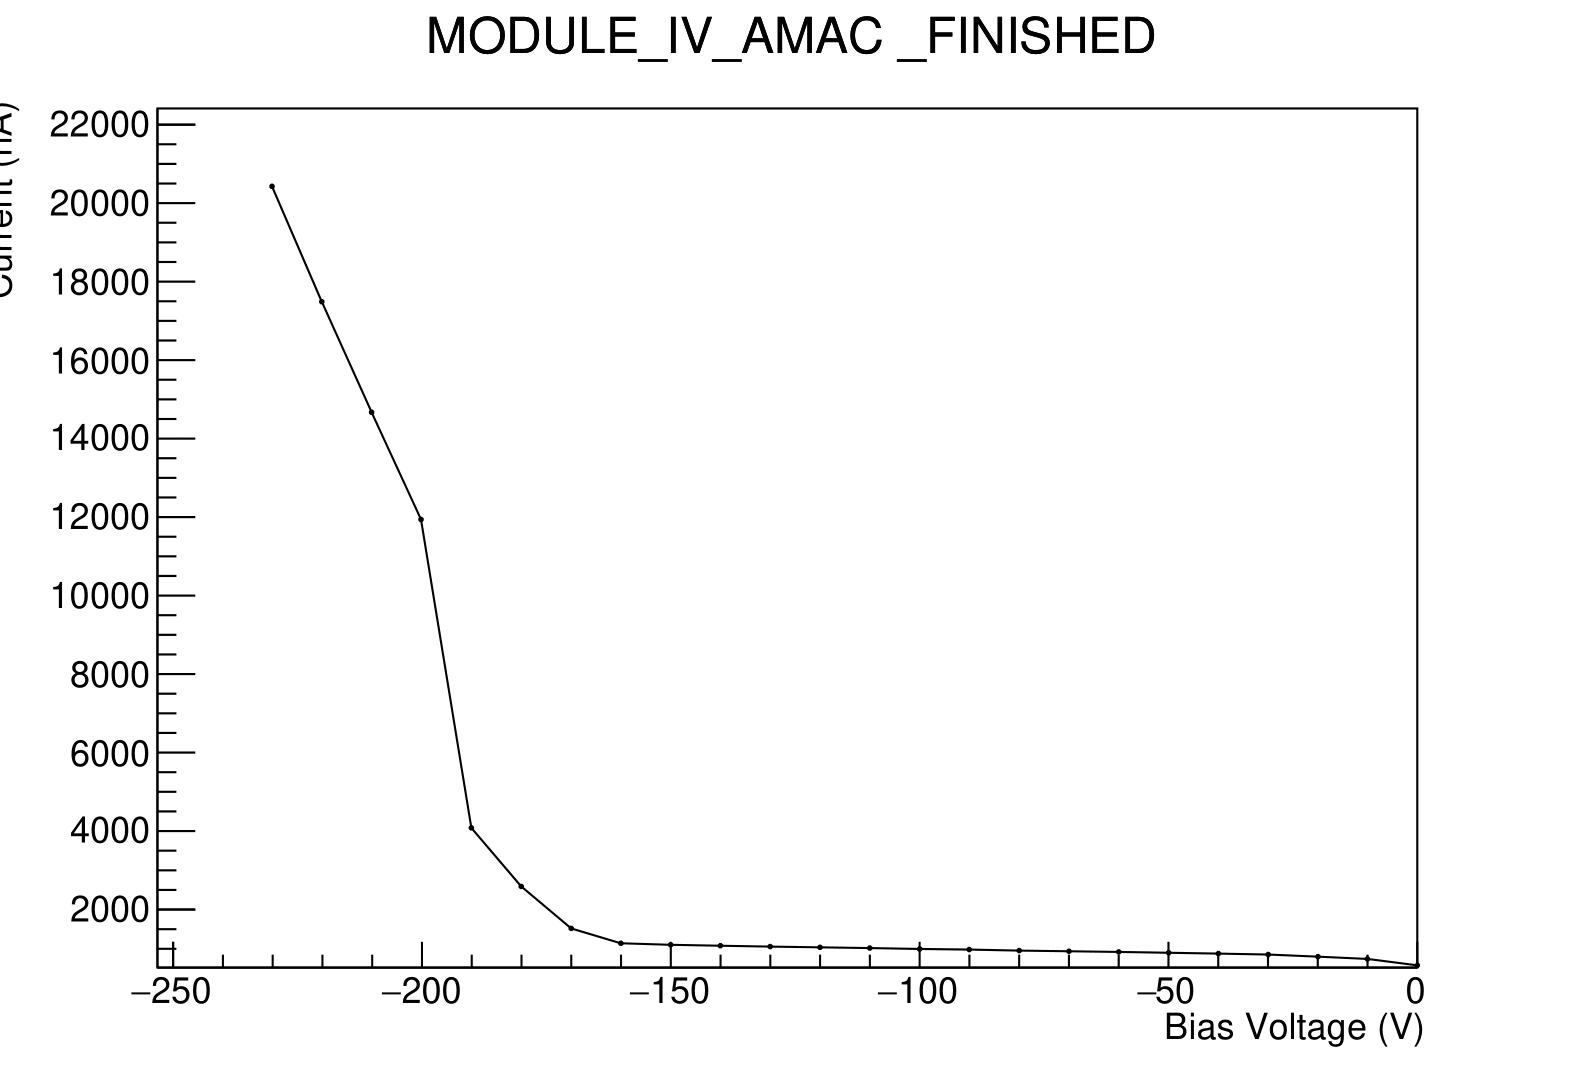
\includegraphics[width=7cm,height=8cm,keepaspectratio]{Figures/test/IV1.png}
        \caption{}\label{fig:IV1}
    \end{subfigure}
    ~
    \begin{subfigure}[b]{0.45\textwidth}
        \centering
        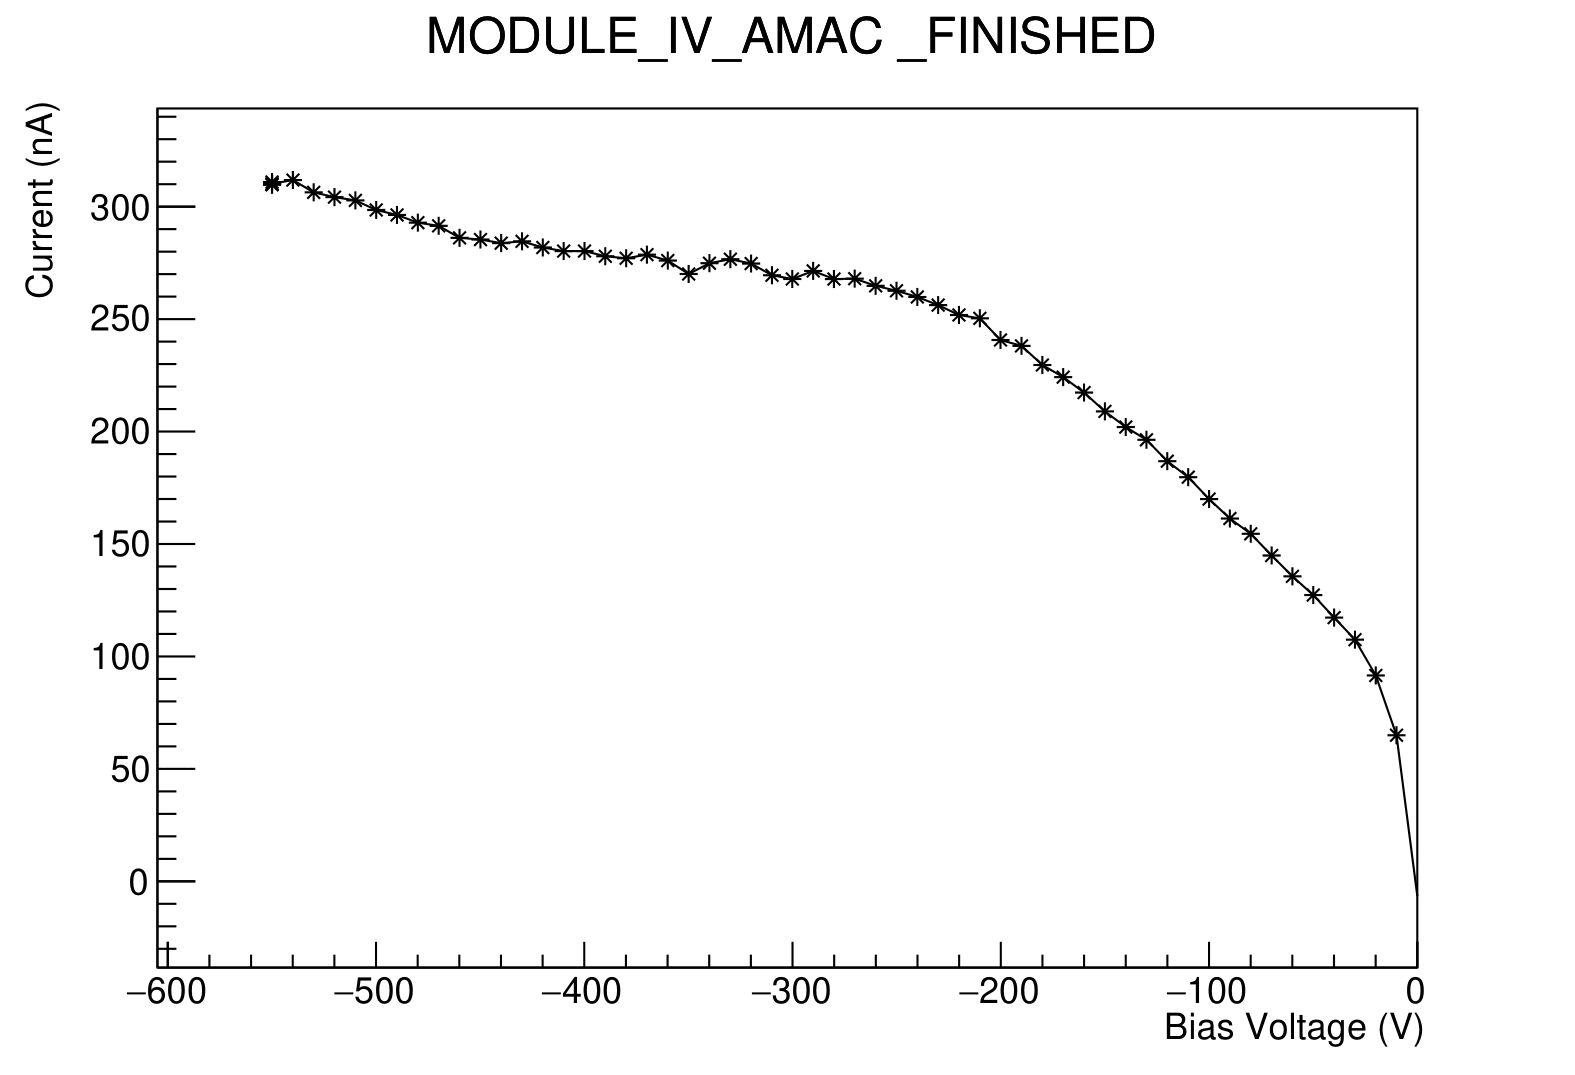
\includegraphics[width=7cm,height=8cm,keepaspectratio]{Figures/test/IV2.png}
        \caption{}\label{fig:IV2}
    \end{subfigure}
    \caption{Example plots of I-V test of a) a faulty module with a sharp breaking point of current at $-170 \si{\volt}$, and b) a healthy module with a consistent current compared to decreased voltage}
    \label{fig:IV}
\end{figure}

\textcolor{blue}{For the ITk end-cap modules, the operation voltage of $-350 \si{\volt}$ for the starting point, and the maximum of $-500 \si{\volt}$ during the late lifetime of the modules is foreseen. Consequently, we then expect a healthy module to show a consistent current without a sharp braking point within this voltage boundary in the I-V test.}







%what are each test show and why are they relevant








%Use kolanoski book
%% Theory

\chapter{Theory} % Main chapter title

\label{Theory} % For referencing the chapter elsewhere, use \ref{Theory} 

%----------------------------------------------------------------------------------------

% Define some commands to keep the formatting separated from the content 
\newcommand{\keyword}[1]{\textbf{#1}}
\newcommand{\tabhead}[1]{\textbf{#1}}
\newcommand{\code}[1]{\texttt{#1}}
\newcommand{\file}[1]{\texttt{\bfseries#1}}
\newcommand{\option}[1]{\texttt{\itshape#1}}

%----------------------------------------------------------------------------------------
A good theory
\section{sec1}
\subsection{sub1}

%TDR 5.4
%TDR 6.1 
% Results

\chapter{Results} % Main chapter title

\label{Results} % For referencing the chapter elsewhere, use \ref{Results} 

%----------------------------------------------------------------------------------------

% Define some commands to keep the formatting separated from the content 
\newcommand{\keyword}[1]{\textbf{#1}}
\newcommand{\tabhead}[1]{\textbf{#1}}
\newcommand{\code}[1]{\texttt{#1}}
\newcommand{\file}[1]{\texttt{\bfseries#1}}
\newcommand{\option}[1]{\texttt{\itshape#1}}

%----------------------------------------------------------------------------------------

During the development stage of the test and data collection, several tests were performed in order to find the relevant data and calibrate the output of the data according to our needs. Following, we will provide the result of two separate full tests which were made to both test the stability of the LTRT process, and after that capture the environmental and AMAC electrical data from InFlux.\footnote{\textcolor{blue}{Please note that the LTRT results shown are from a Pre Production A (PPA) module, and solely presented for the proof of concept and the results do not reflect the validity and functionality of the module.}} \\

 

\begin{figure}[h]
    \centering
    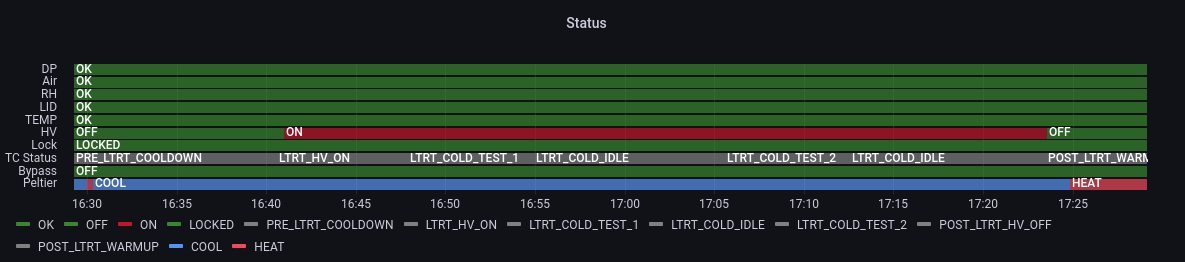
\includegraphics[width=14cm,height=11cm,keepaspectratio]{Figures/results/test_period.png}
    \caption{A record of two consecutive LTRT tests in the Influx database, showing the pre-tests, the LTRT test, and the waiting (IDLE) period between each test.}
    \label{fig:LTRTinflux}
\end{figure}

The first test was performed at $0 \si{\celsius}$ with $2$ iteration of LTRT and an interval of $10$ minutes between the two cold LTRTs. The timetable related to this test is shown in Fig\ref{fig:LTRTinflux}. The results of the ABCstar full test are shown in Fiq.\ref{fig:LTRT_result_1} and Fiq.\ref{fig:LTRT_result_2} showing the result of the two attempts of the performed test. (and Fiq.\ref{fig:LTRT_result_1_large} and Fiq.\ref{fig:LTRT_result_2_large} for higher resolution)

\begin{figure}[h]
    \centering
    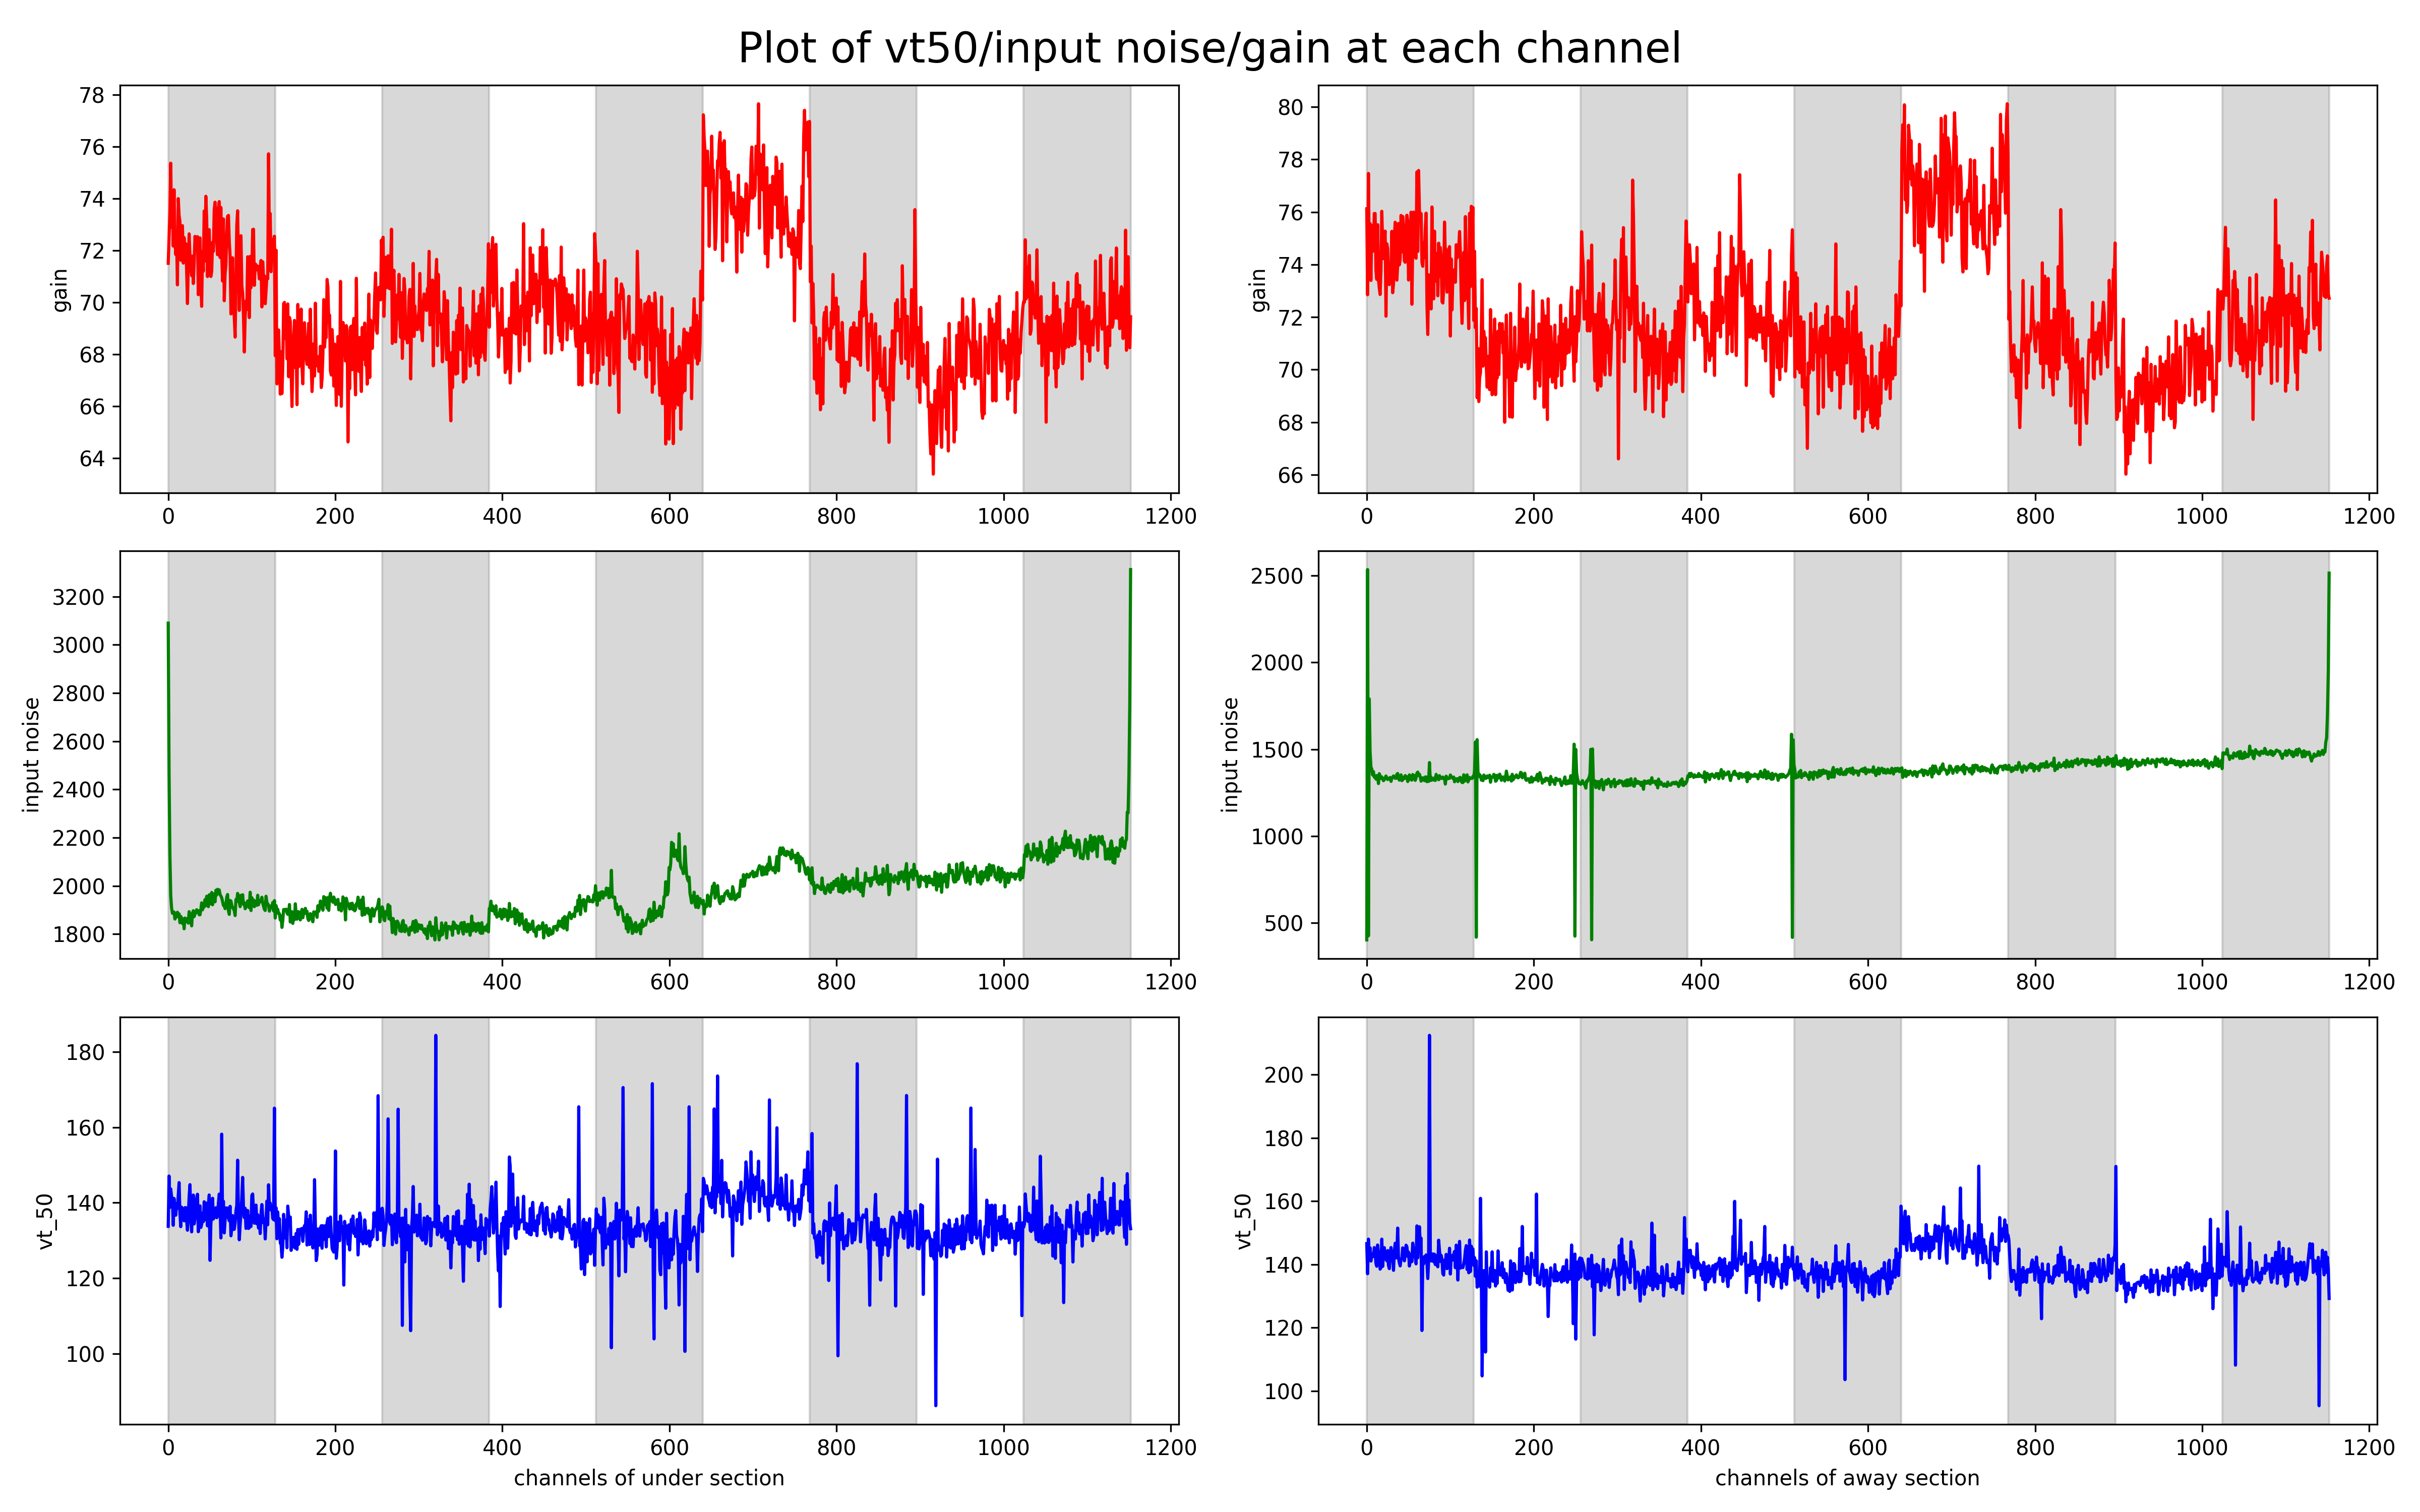
\includegraphics[width=7cm,height=10cm,keepaspectratio]{Figures/results/LTRT_1_plot.png}
    \caption{Plots of $3$ performed electrical test by ABCstar full test during the "LTRT COLD TEST 1" stage, showing the result of VT$50$, input noise, and gain for two hybrids (under and above) of a Pre Production A (PPA) R5 module.}
    \label{fig:LTRT_result_1}
\end{figure}

\begin{figure}[h]
    \centering
    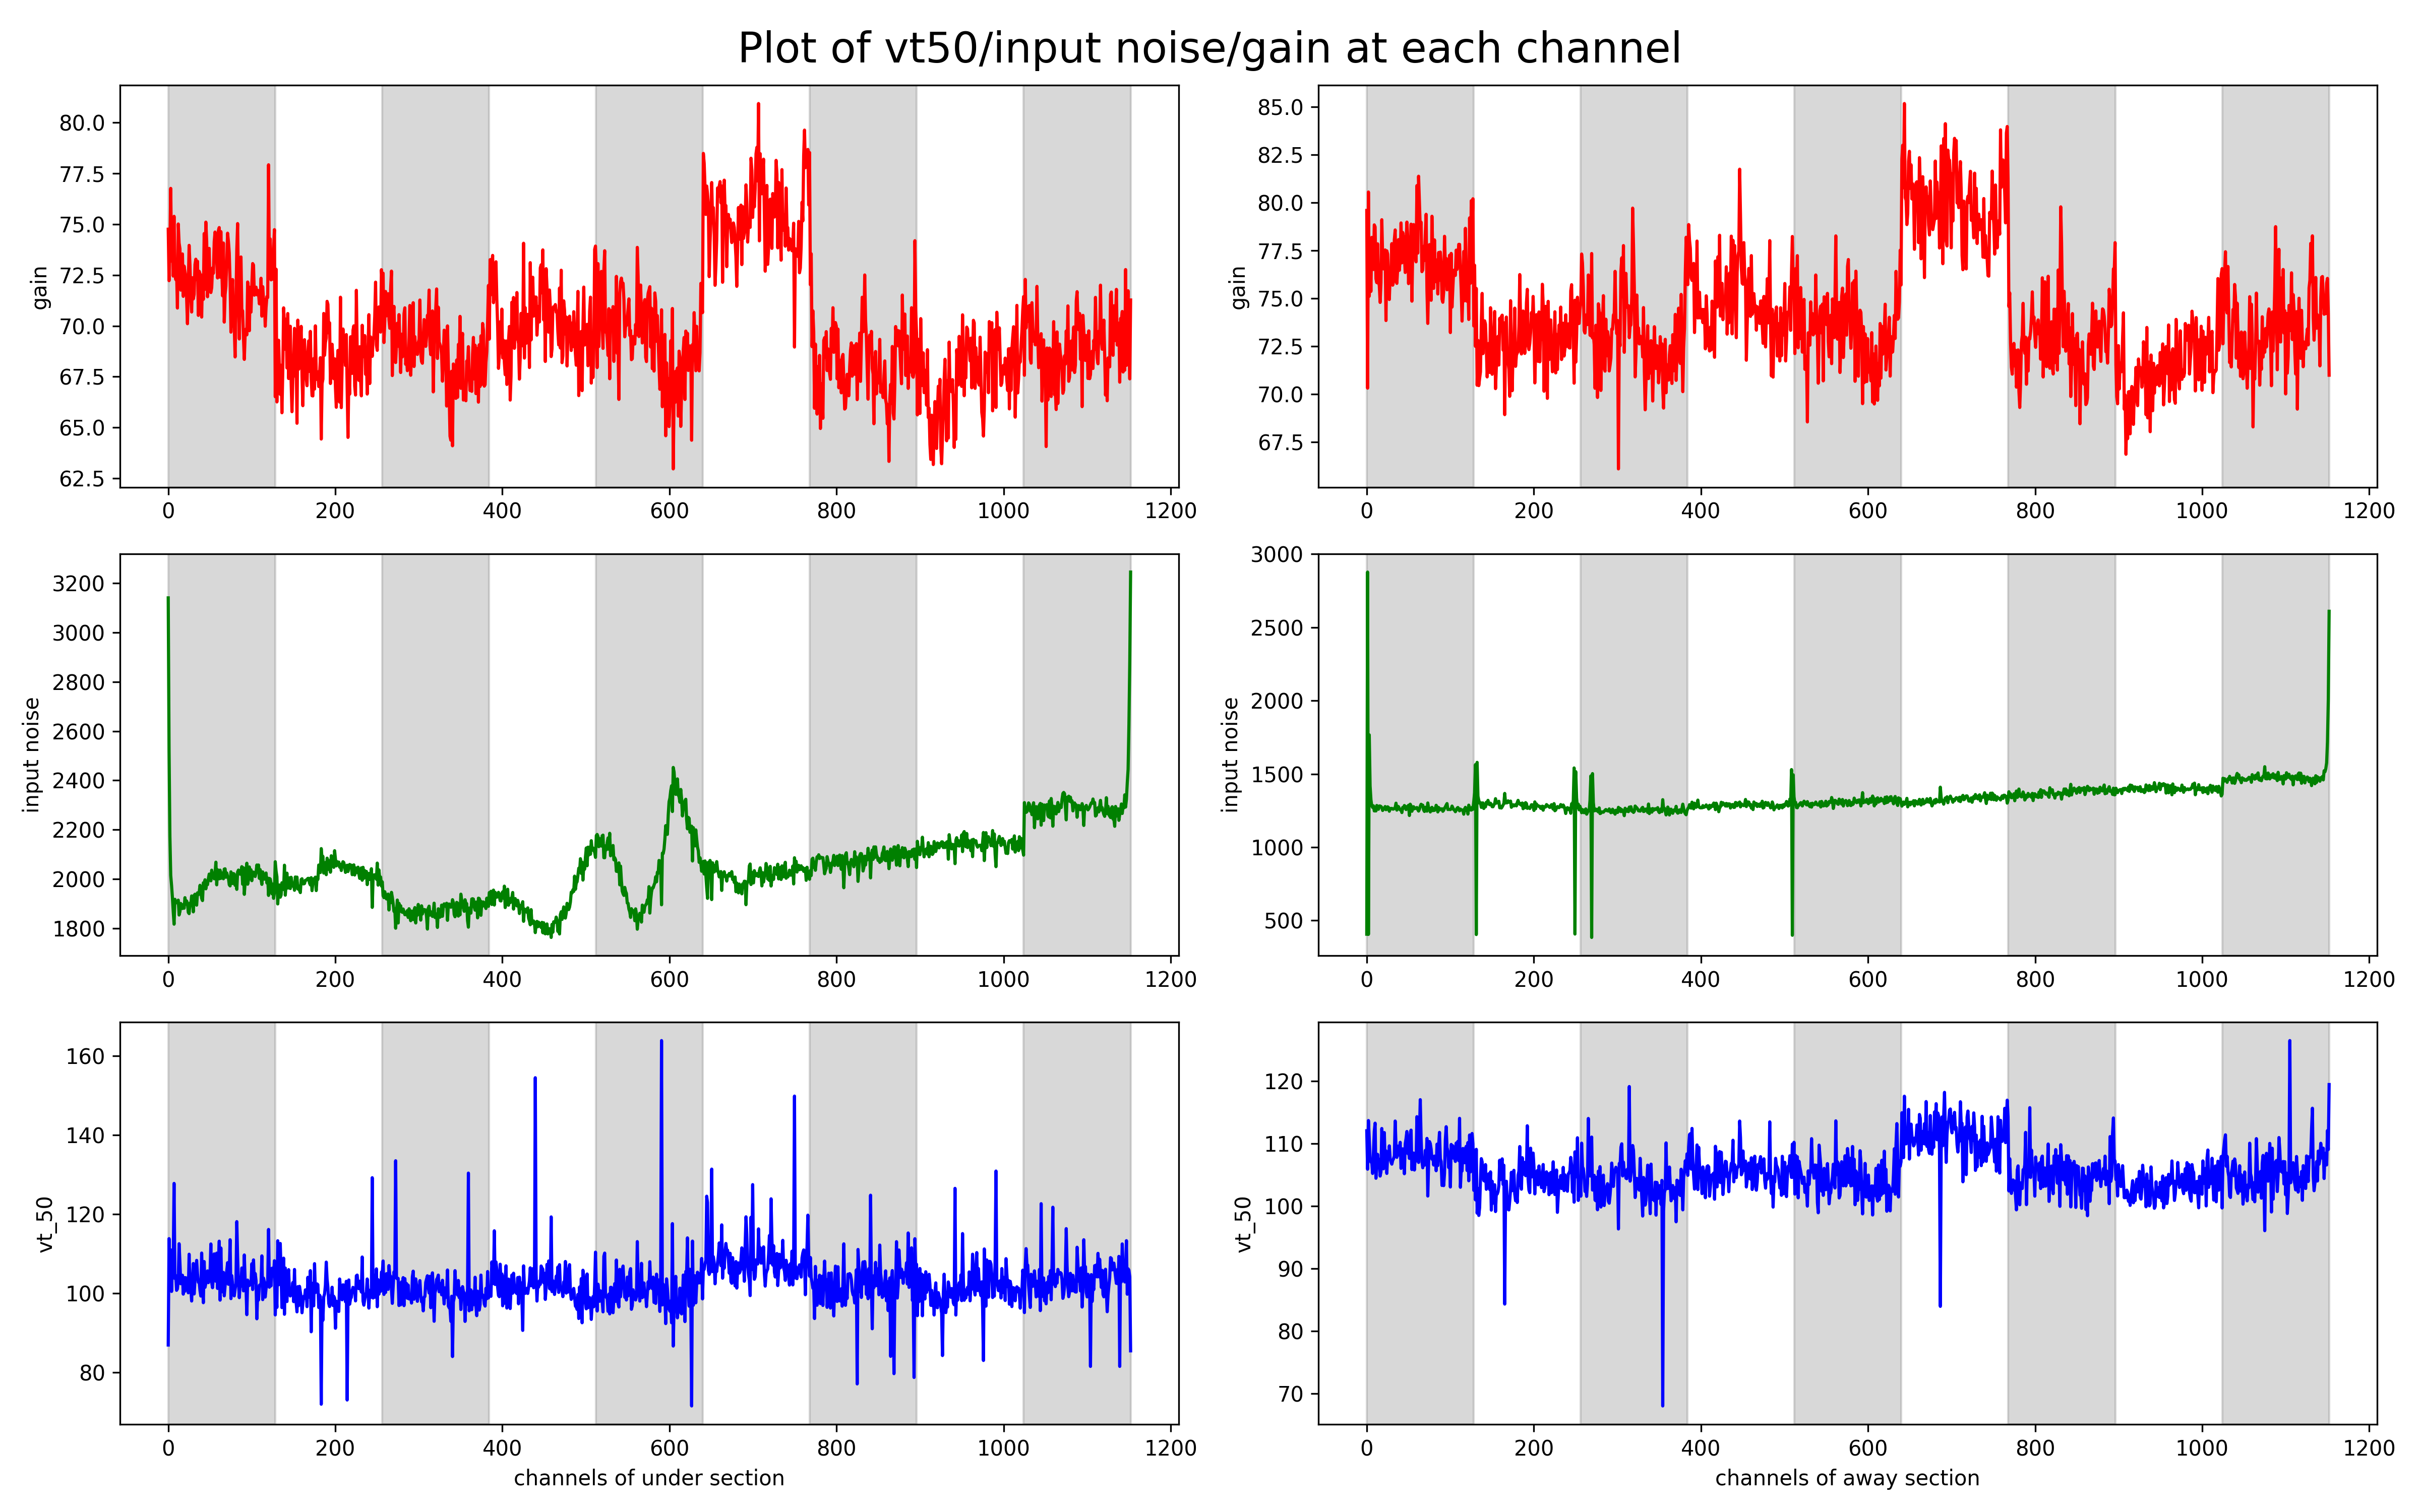
\includegraphics[width=7cm,height=10cm,keepaspectratio]{Figures/results/LTRT_2_plot.png}
    \caption{Plots of $3$ performed electrical test by ABCstar full test during the "LTRT COLD TEST 2" stage, showing the result of VT$50$, input noise, and gain for two hybrids (under and above) of a Pre Production A (PPA) R5 module.}
    \label{fig:LTRT_result_2}
\end{figure}

Each point in the plots above shows the value of a single channel, and each highlighted area divides the data from each ABCstar readout (for this case $9$ readout per hybrid).\\

The environmental data related to both "LTRT COLD TEST 1" and "LTRT COLD TEST 2" and the "IDLE" period in between two tests is shown in Fig.\ref{fig:env_1}(and Fiq.\ref{fig:env_1_large} for higher resolution)

\begin{figure}[h]
    \centering
    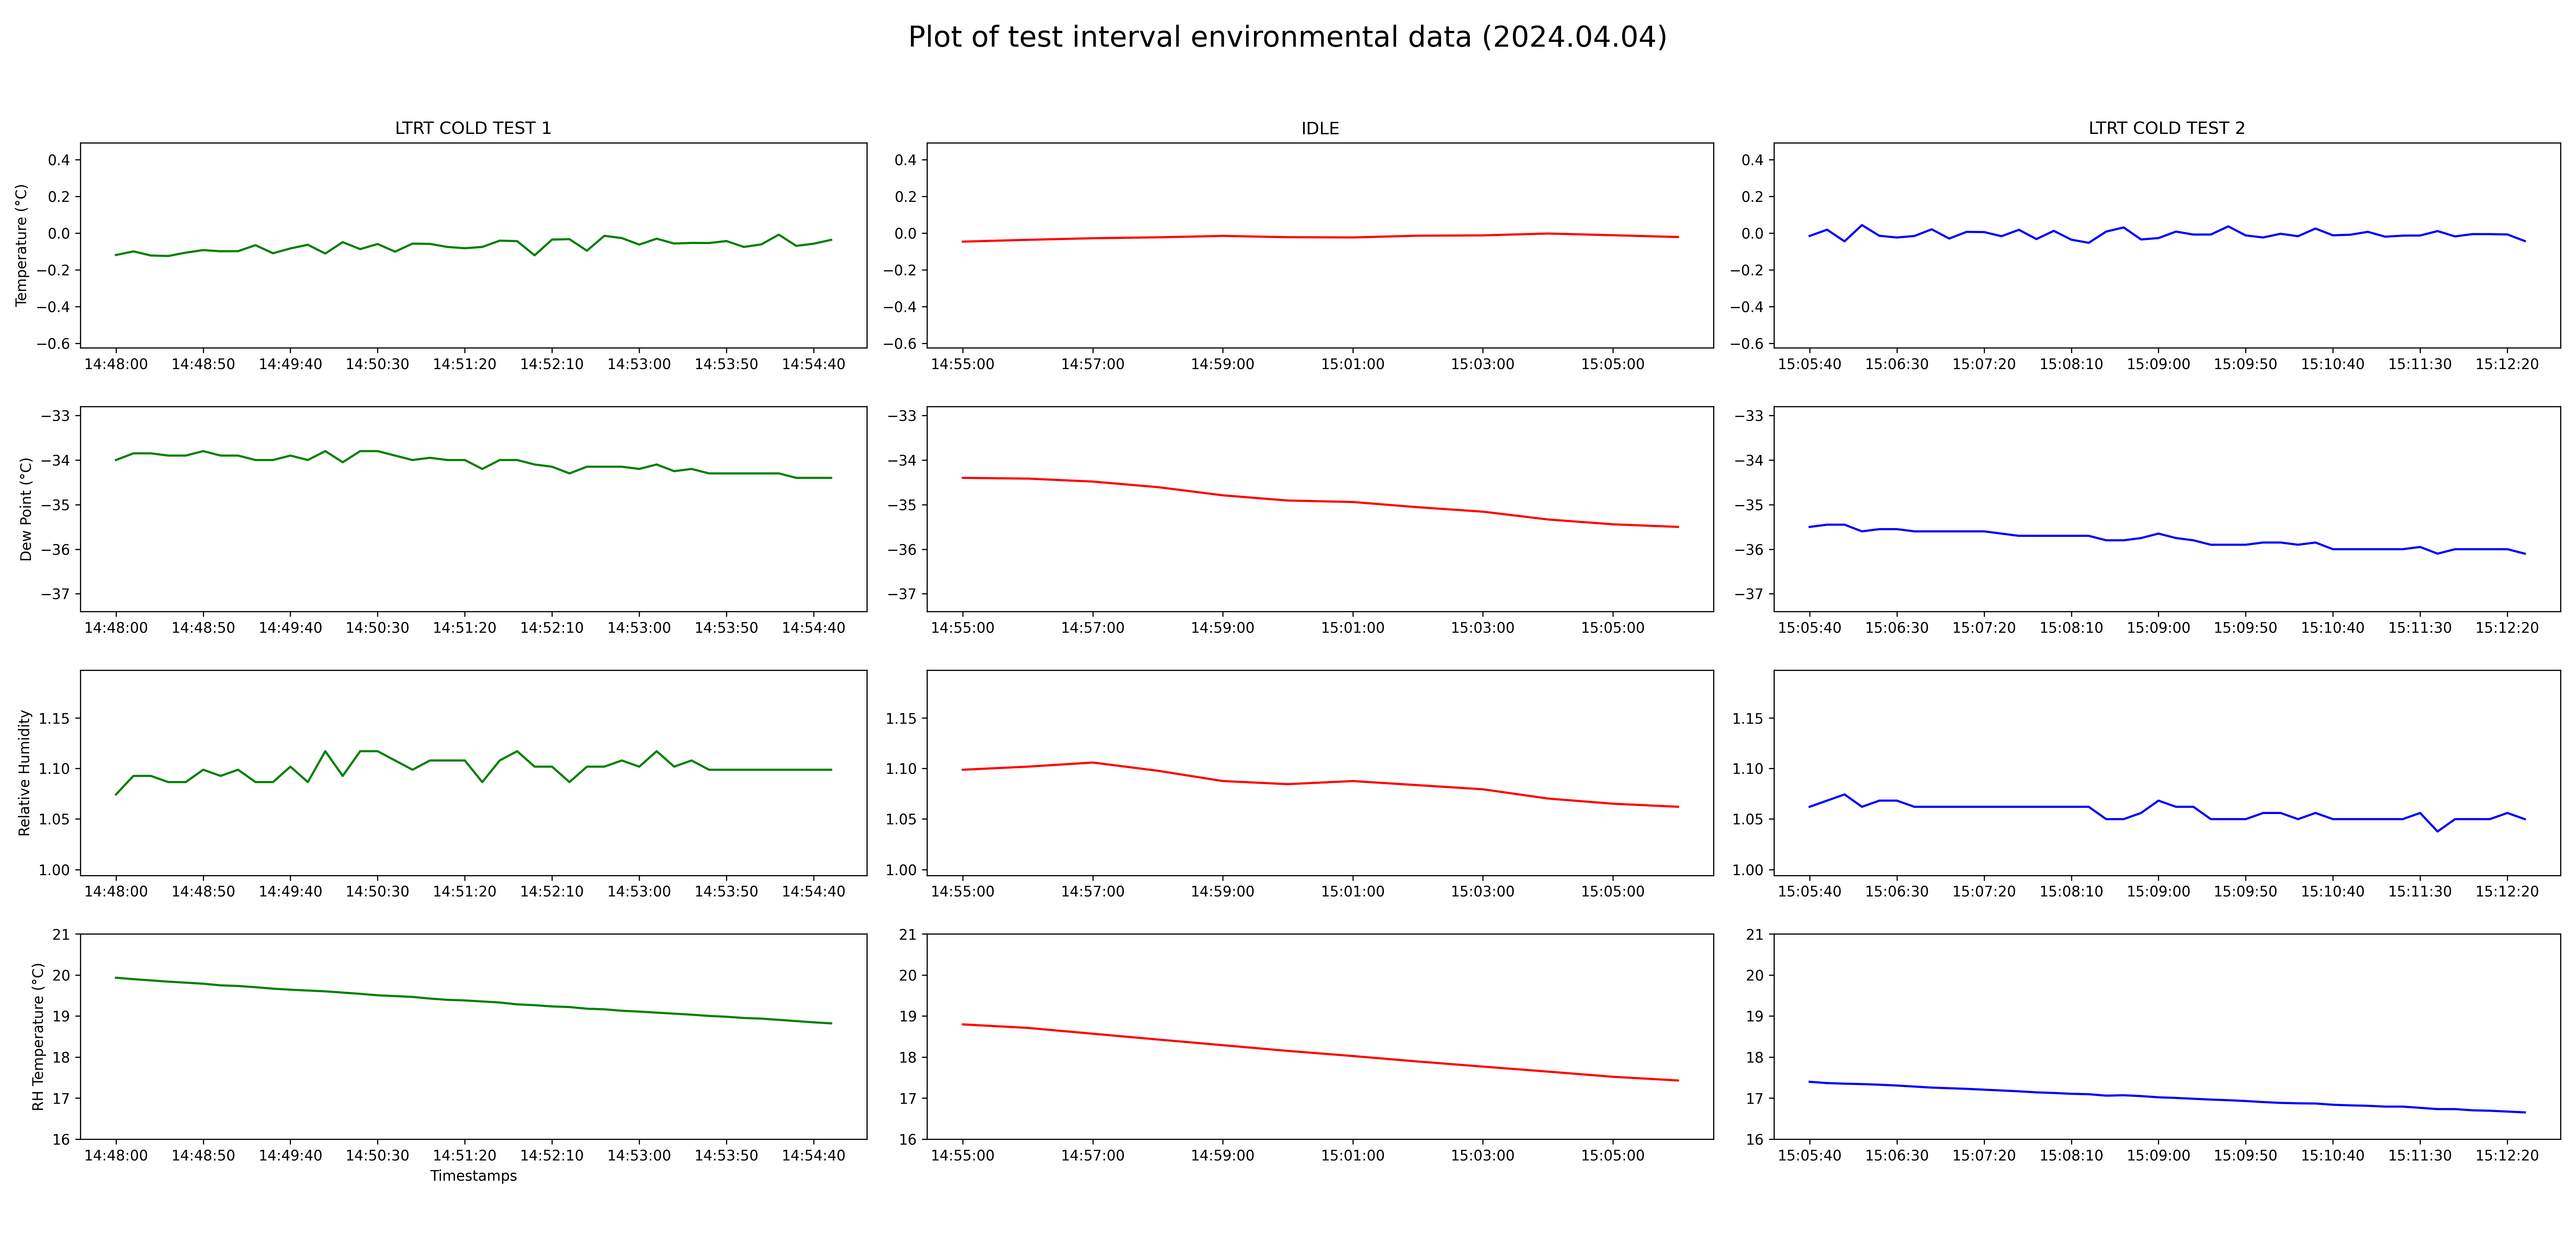
\includegraphics[width=12cm,height=10cm,keepaspectratio]{Figures/results/env_plot_20240404_.png}
    \caption{Plots environmental data during the time span of the LTRT test shown in Fig.\ref{fig:LTRT_result_1} including the data for Temperature, Dew point, Relative humidity, and Relative humidity temperature.}
    \label{fig:env_1}
\end{figure}

The AMAC electrical data related to this test is shown in Fig.\ref{fig:amac_1}(and Fiq.\ref{fig:amac_1_large} for higher resolution)

\begin{figure}[h]
    \centering
    \includegraphics[width=12cm,height=10cm,keepaspectratio]{Figures/results/amac_plot_20240404_.png}
    \caption{Plots AMAC electrical data during the time span of the LTRT test shown in Fig.\ref{fig:LTRT_result_1} including the data for input and output currents and voltage.}
    \label{fig:amac_1}
\end{figure}

While the time taken for each test varies depending on the module, configuration, and settings, by aligning the ordered tests with the environmental and electrical data, we can have a general overview of the test conditions. \\
By checking the environmental plots we can determine that the temperature on the chuck which the module was installed on, was perfectly constant during the LTRT COLD TESTs and the IDLE period and was maintained at $0\si{\celsius}$. The dew point, however, is decreasing. Since the dew point is directly proportional to relative humidity and the air temperature, we can see that this change is a result of the decrease in relative humidity during the full test. Although the air temperature (RH Temp.) showing step-like decrease during each stage, but the   
%% Discussion

\chapter{Discussion} % Main chapter title

\label{Discussion} % For referencing the chapter elsewhere, use \ref{Discussion} 

%----------------------------------------------------------------------------------------

% Define some commands to keep the formatting separated from the content 
\newcommand{\keyword}[1]{\textbf{#1}}
\newcommand{\tabhead}[1]{\textbf{#1}}
\newcommand{\code}[1]{\texttt{#1}}
\newcommand{\file}[1]{\texttt{\bfseries#1}}
\newcommand{\option}[1]{\texttt{\itshape#1}}

%---------------------------------------------------------------------------------------- 
%% Conclusion

\chapter{Conclusion} % Main chapter title

\label{Conclusion} % For referencing the chapter elsewhere, use \ref{Conclusion} 

%----------------------------------------------------------------------------------------

% Define some commands to keep the formatting separated from the content 
\newcommand{\keyword}[1]{\textbf{#1}}
\newcommand{\tabhead}[1]{\textbf{#1}}
\newcommand{\code}[1]{\texttt{#1}}
\newcommand{\file}[1]{\texttt{\bfseries#1}}
\newcommand{\option}[1]{\texttt{\itshape#1}}

%----------------------------------------------------------------------------------------
%possible improvement to the system
%Further work
%outlook
 

%----------------------------------------------------------------------------------------
%	THESIS CONTENT - APPENDICES
%----------------------------------------------------------------------------------------

\appendix % Cue to tell LaTeX that the following "chapters" are Appendices

% Include the appendices of the thesis as separate files from the Appendices folder
% Uncomment the lines as you write the Appendices

\chapter{Additional figures and plots} % Main appendix title

\label{AppendixA} % Change X to a consecutive letter; for referencing this appendix elsewhere, use \ref{AppendixX}

%More figures for other parts of the detector

%ITK layout
\section{ITK detector and modules layout}
\begin{figure}[h]
    \centering
    \includegraphics[width=12cm,height=10cm,keepaspectratio]{Figures/modules/Appendix/layout1.png}
    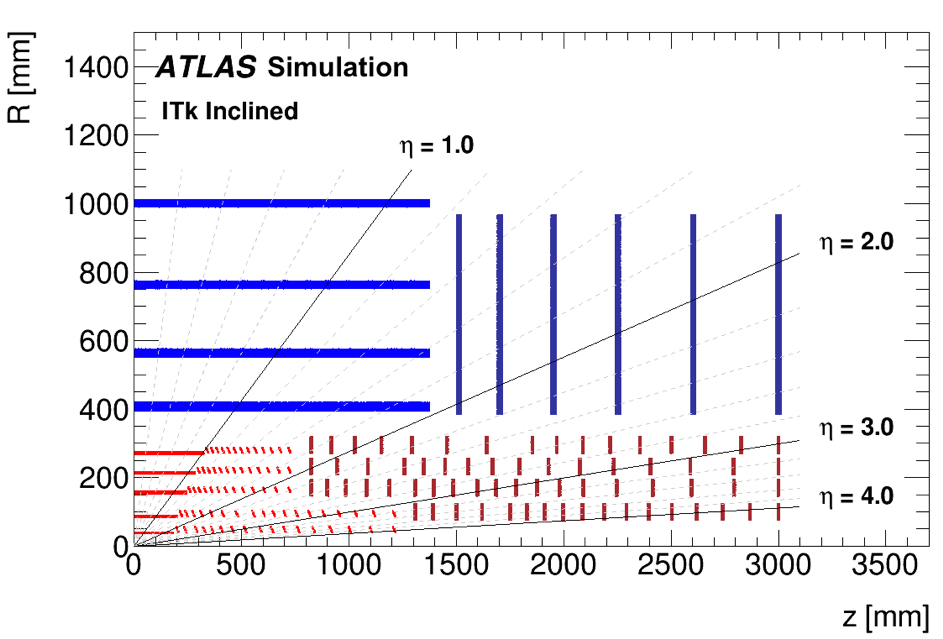
\includegraphics[width=11cm,height=8cm,keepaspectratio]{Figures/modules/Appendix/layout2.png}
    \caption{The Layout of the ITk Strip Detector. The left figure showcases the layout of the detector consisting of $4$ barrel layers (horizontal lines) and $6$ end-cap disks on each side. the point $0$ is the interaction point, and the horizontal axis is the axis along the beam line. Both figures show the rapidity (pseudorapidity) coverage of the ITk detector (red for ITk-Pixel and blue for ITk-Strip) with the barrel part covering $\eta \approx \pm 1.05$ and the total coverage of the detector is $\eta \approx \pm 2.7$\cite{Collaboration:390920} }
    \label{fig:additionalLayout}
\end{figure}

\newpage
\section{Barel and Enc-cap modules}
\begin{figure}[h]
    \begin{subfigure}[b]{1\textwidth}
        \centering
        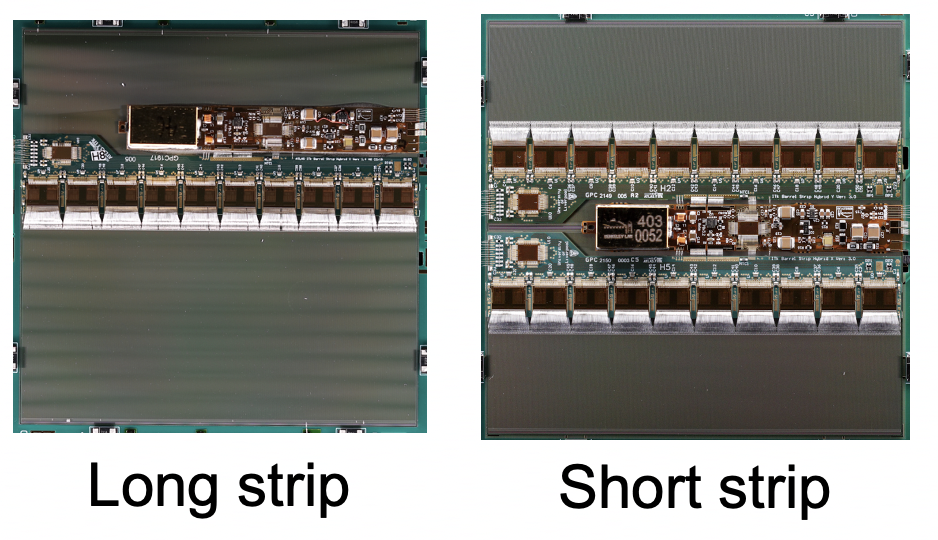
\includegraphics[width=14cm,height=15cm,keepaspectratio]{Figures/modules/Barrel_Modules.png}
        \caption{}\label{fig:barrel}
    \end{subfigure}
    \\
    \begin{subfigure}[b]{1\textwidth}
        \centering
        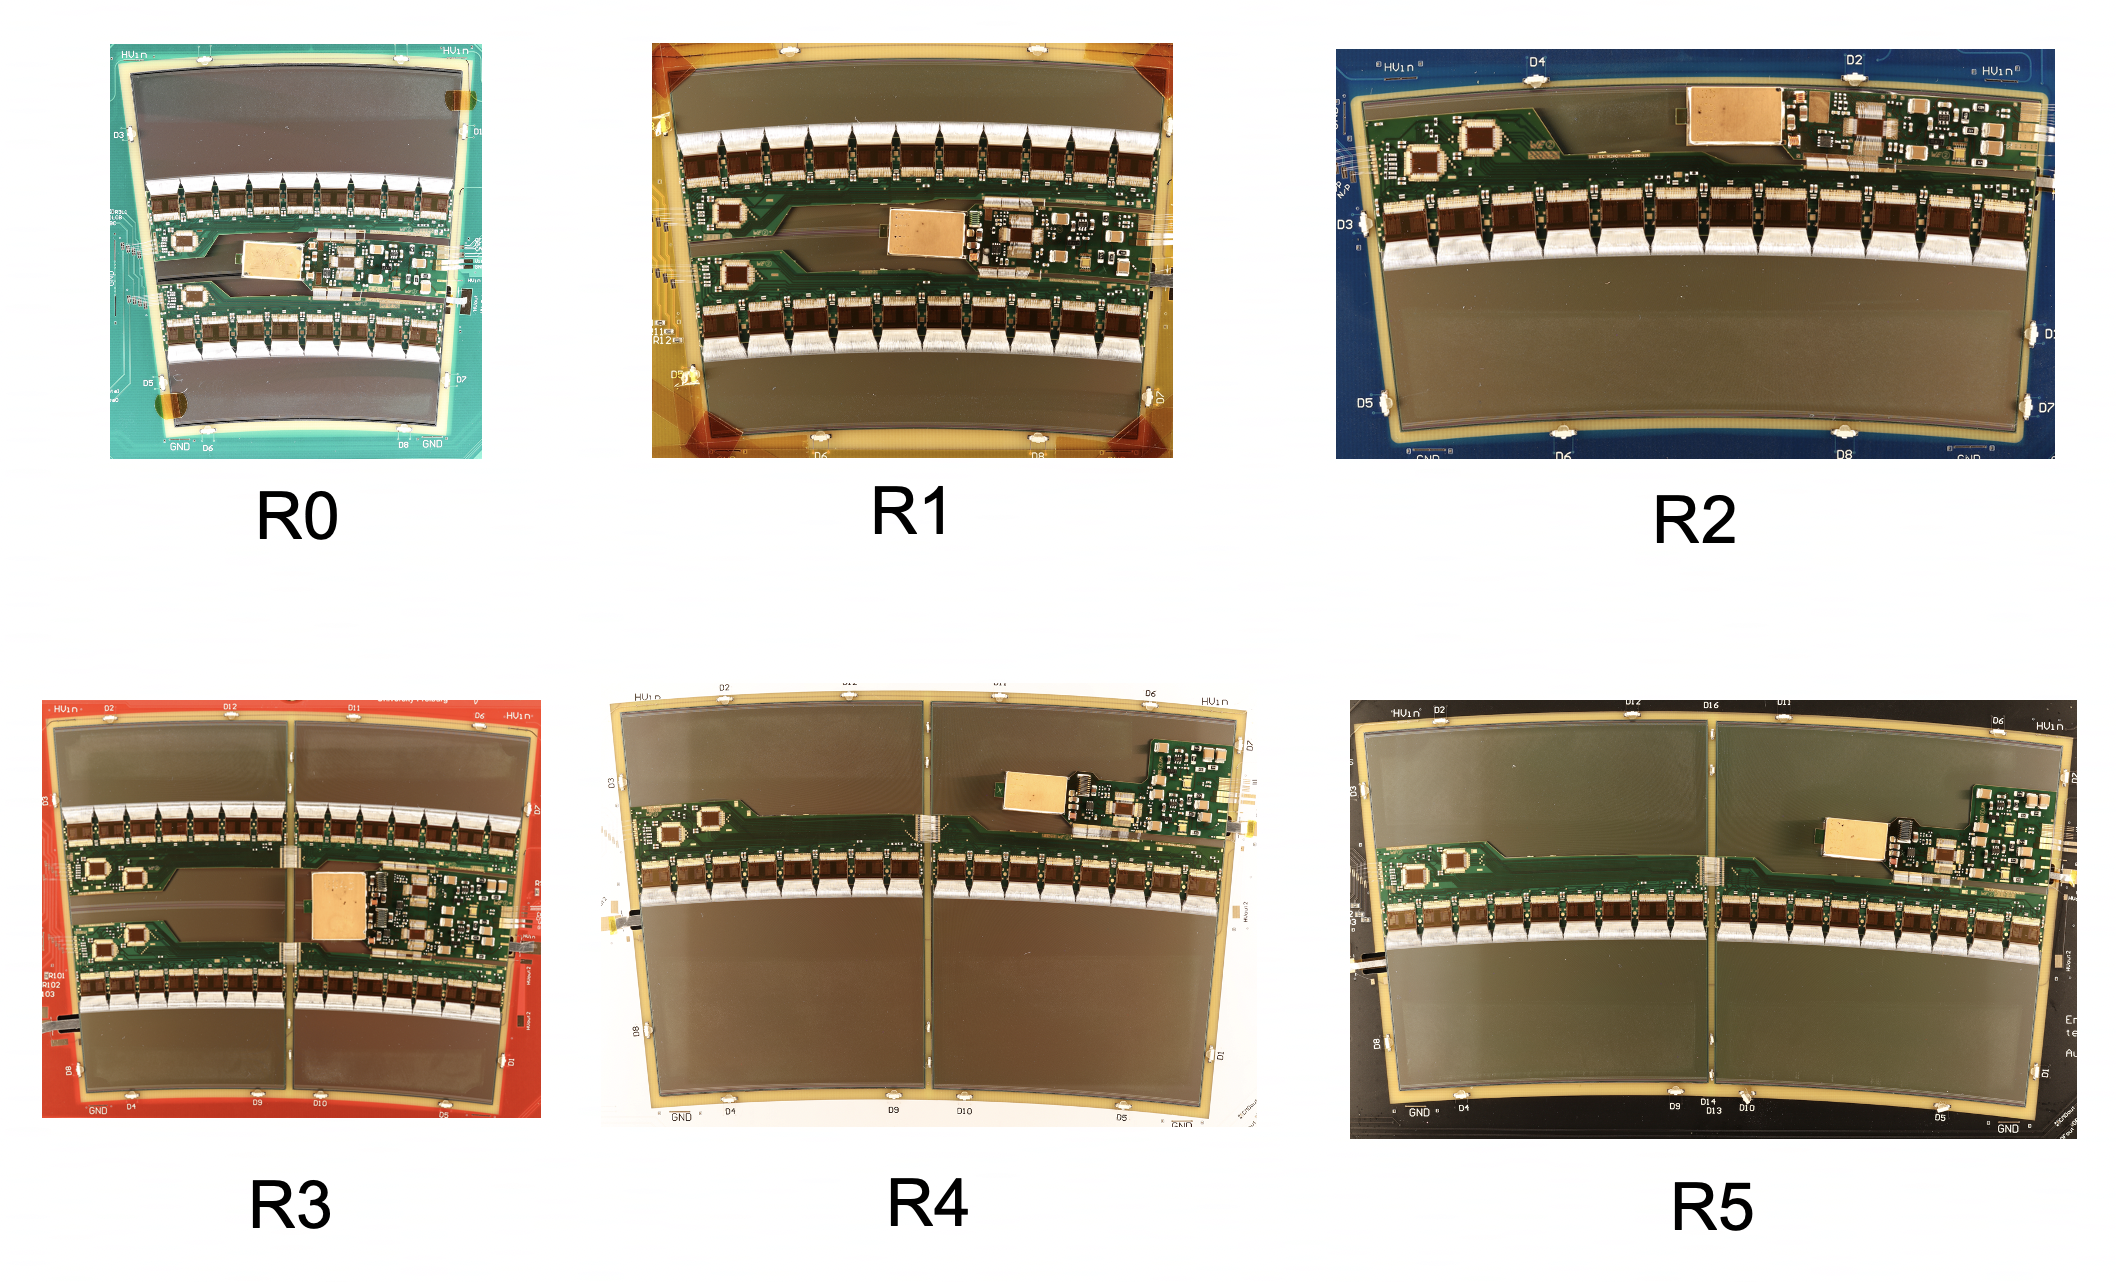
\includegraphics[width=14cm,height=15cm,keepaspectratio]{Figures/modules/EC_Modules.png}
        \caption{}\label{fig:endcap}
    \end{subfigure}
        \caption{Top view pictures of a) barrel modules including LS and SS, and b) end-cap modules including R0 to R5\cite{tishelman2024quality} }
        \label{fig:picModules-large}
\end{figure}

\newpage
\section{Coldbox}
\subsection{Power supllies}
\begin{figure}[h]
    \centering
    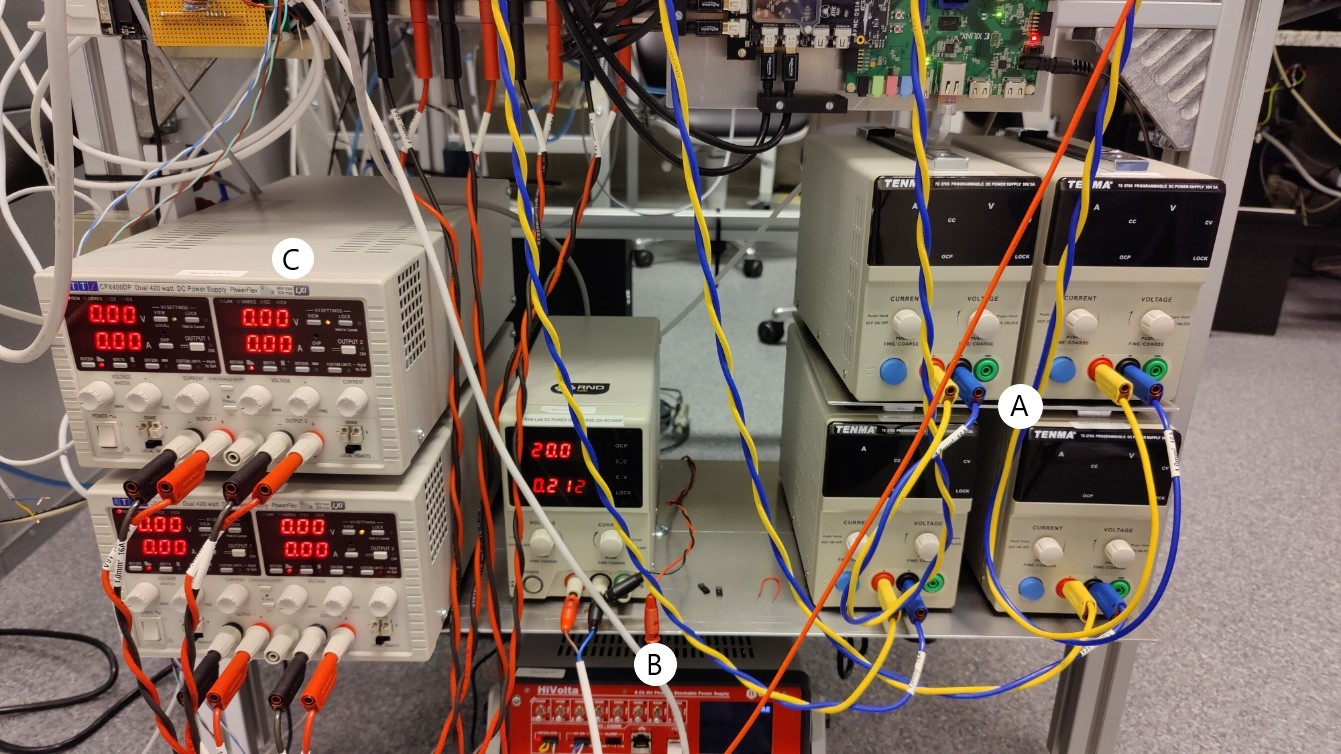
\includegraphics[width=14cm,height=11cm,keepaspectratio]{Figures/test/p-supplies.jpg}
    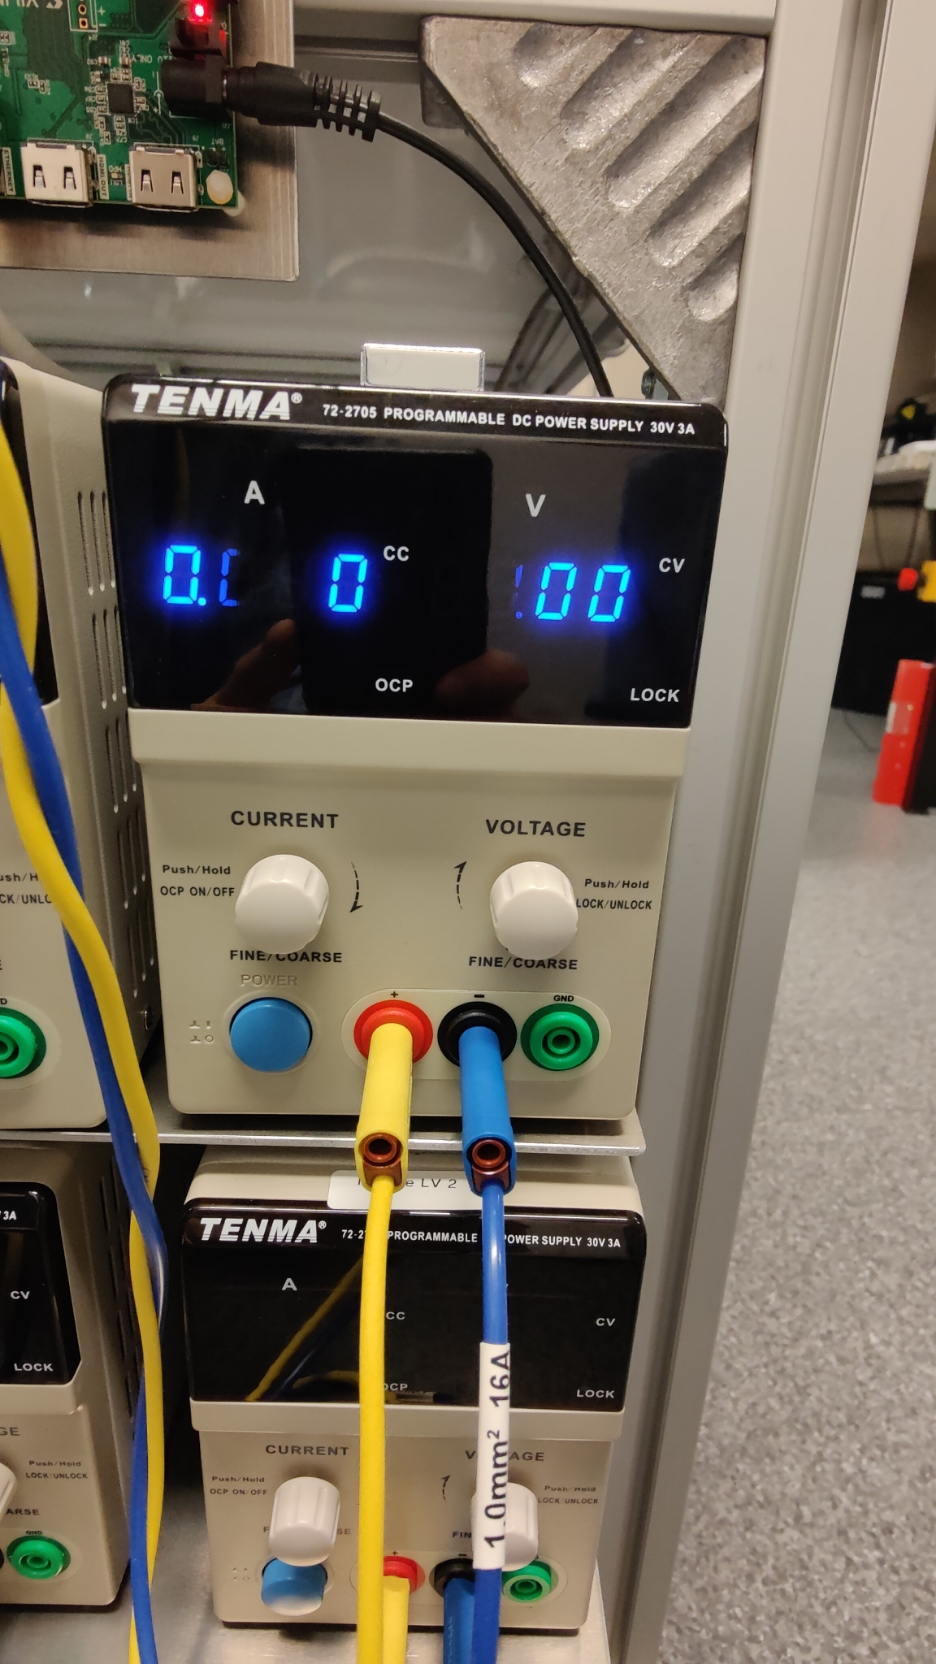
\includegraphics[width=7cm,height=7cm,keepaspectratio]{Figures/test/LV.jpg}
    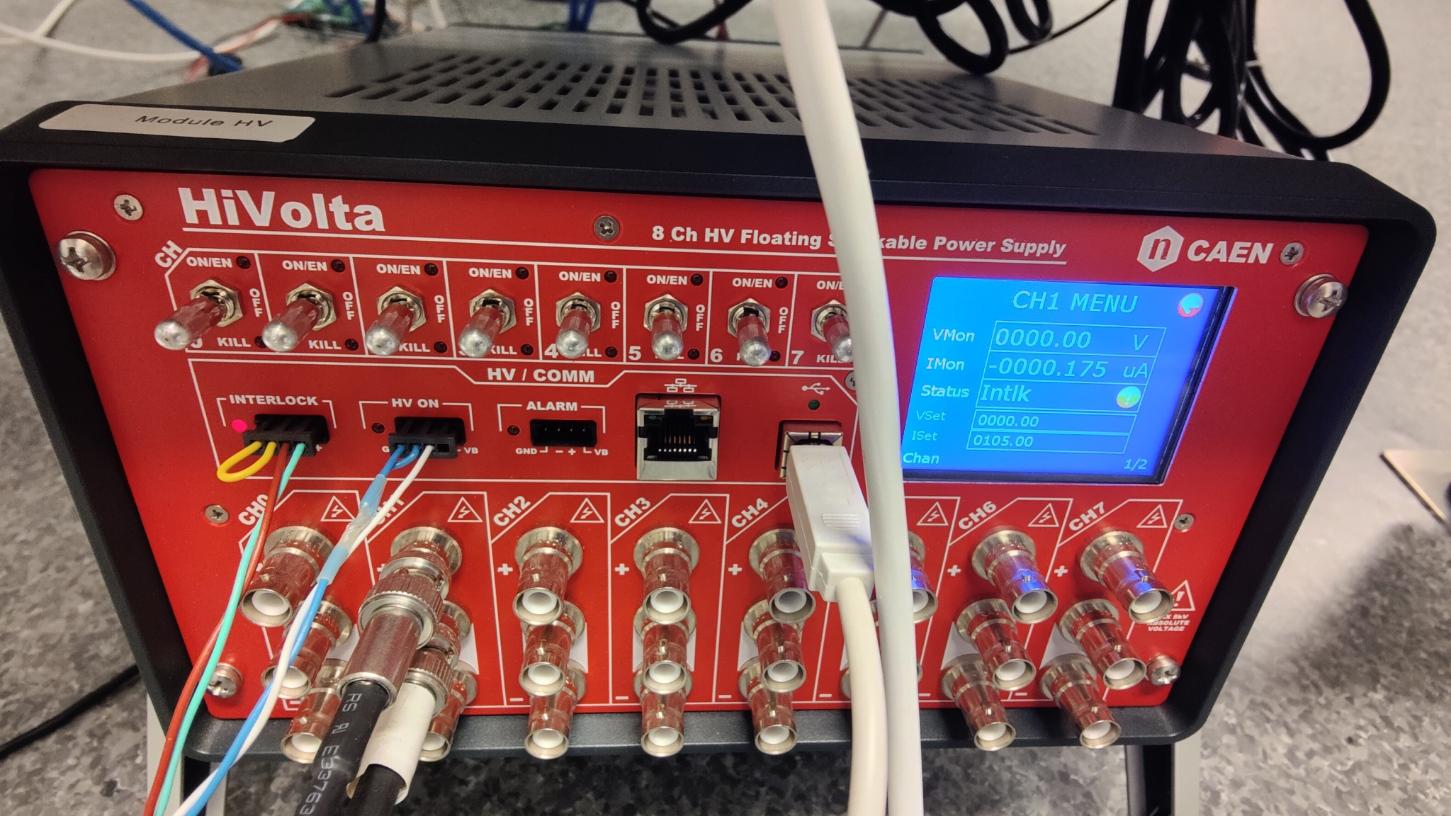
\includegraphics[width=10cm,height=10cm,keepaspectratio]{Figures/test/HV.jpg}
    
    \caption{Pictures of the power supplies: a) Low Voltage used to power the modules, b) High Voltage power supply to inject the test charge, and c) Peltier power supplies}
    \label{fig:supplies}
\end{figure}
\newpage
\subsection{Temperature and air flow}
\begin{figure}[h]
    \centering
    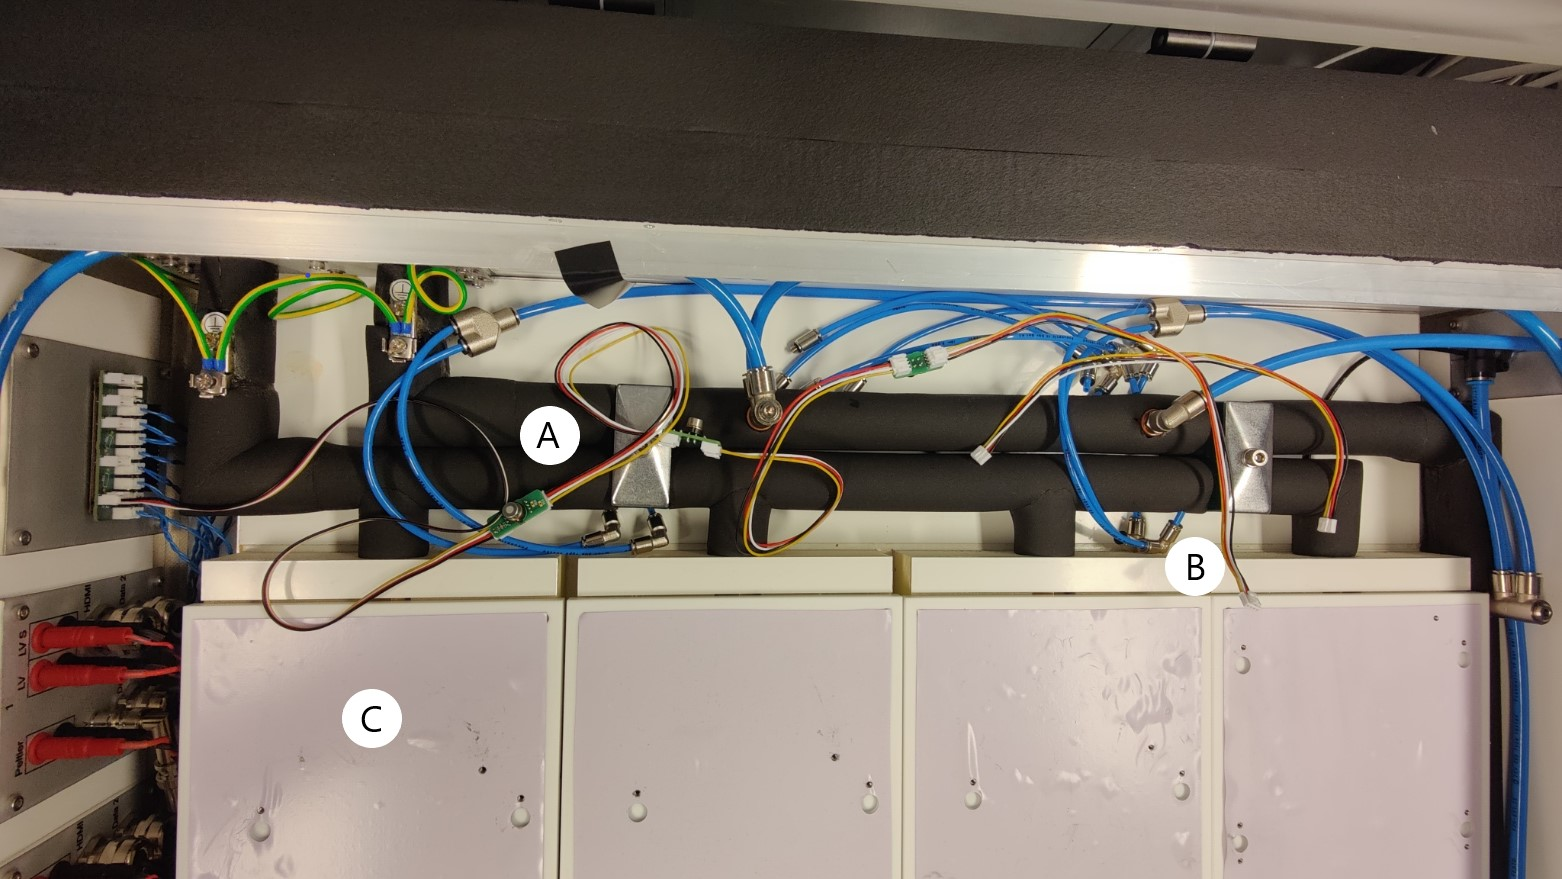
\includegraphics[width=10cm,height=11cm,keepaspectratio]{Figures/test/connections-2.jpg}
    \caption{An overview of the chiller and airflow connections showing a) chiller connections to each chuck using thermally isolated copper pipes, b) airflow connections, and c) Peltiers.}
    \label{fig:cooling}
\end{figure}
\begin{figure}[h]
    \begin{subfigure}[b]{0.45\textwidth}
        \centering
        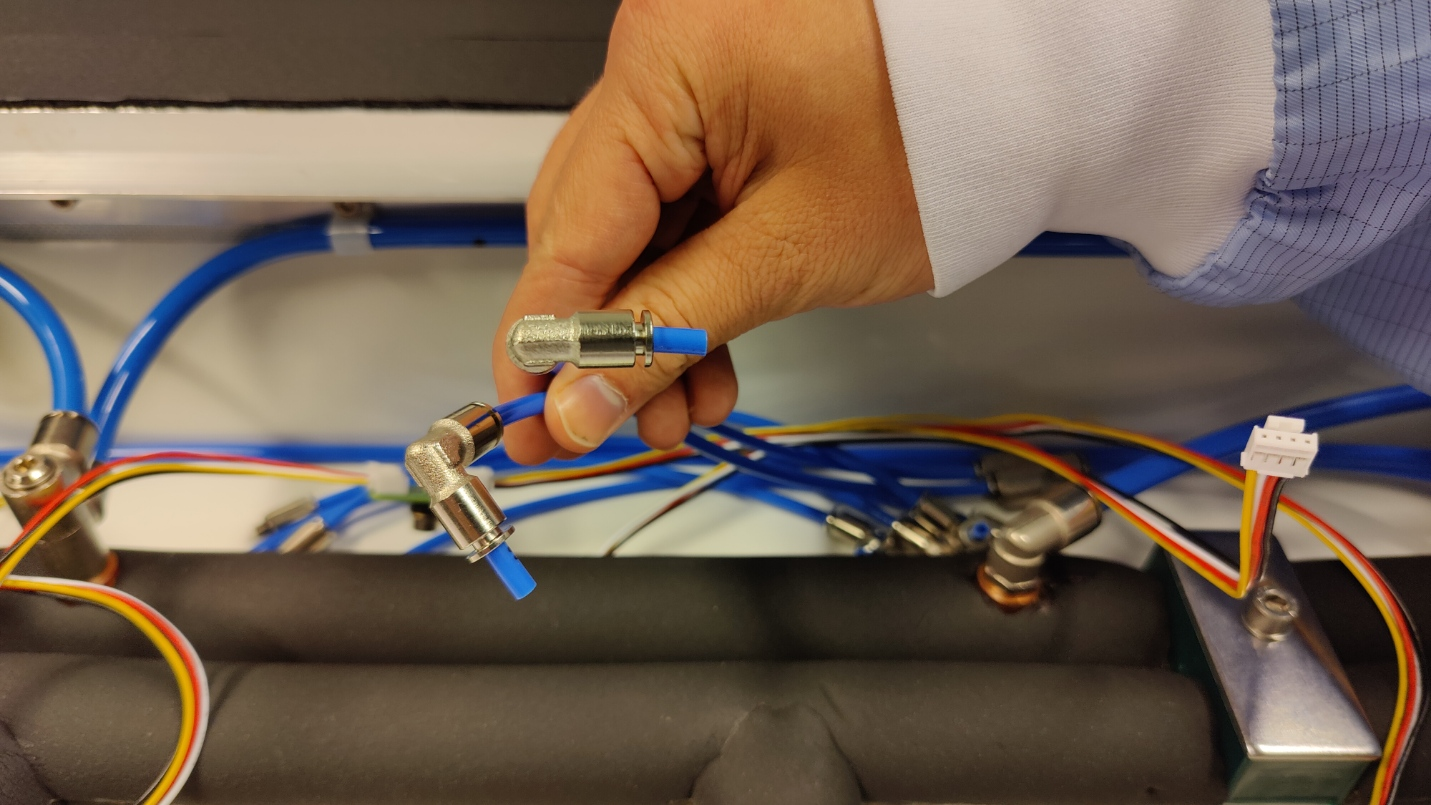
\includegraphics[width=7.5cm,height=10cm,keepaspectratio]{Figures/test/airflow-1.jpg}
        \caption{}\label{fig:airflow1}
    \end{subfigure}
    ~
    \begin{subfigure}[b]{0.45\textwidth}
        \centering
        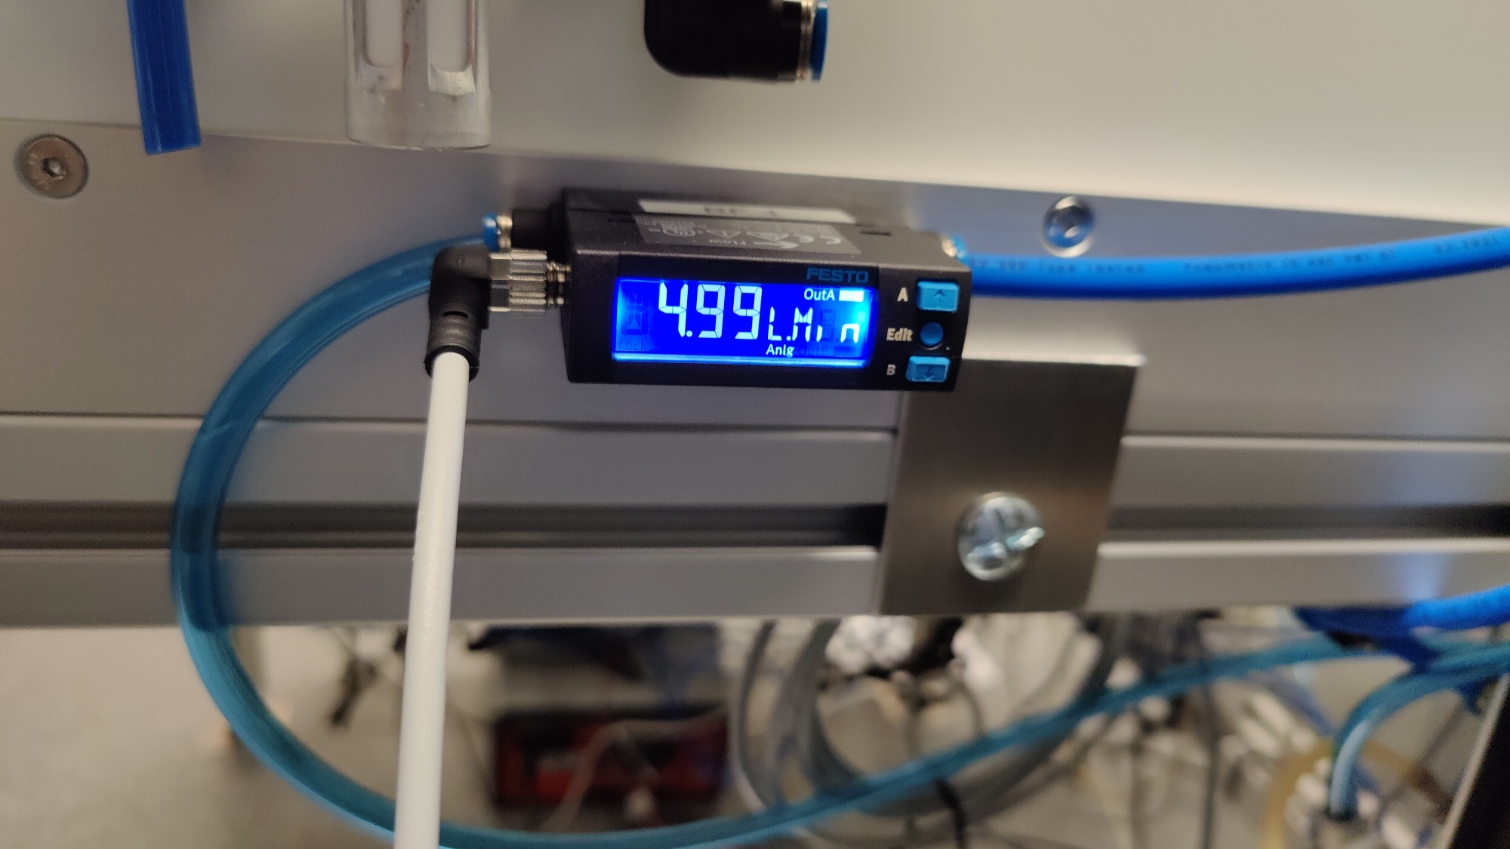
\includegraphics[width=7.5cm,height=10cm,keepaspectratio]{Figures/test/airflow-2.jpg}
        \caption{}\label{fig:airflow2}
    \end{subfigure}

    \begin{subfigure}[b]{0.45\textwidth}
        \centering
        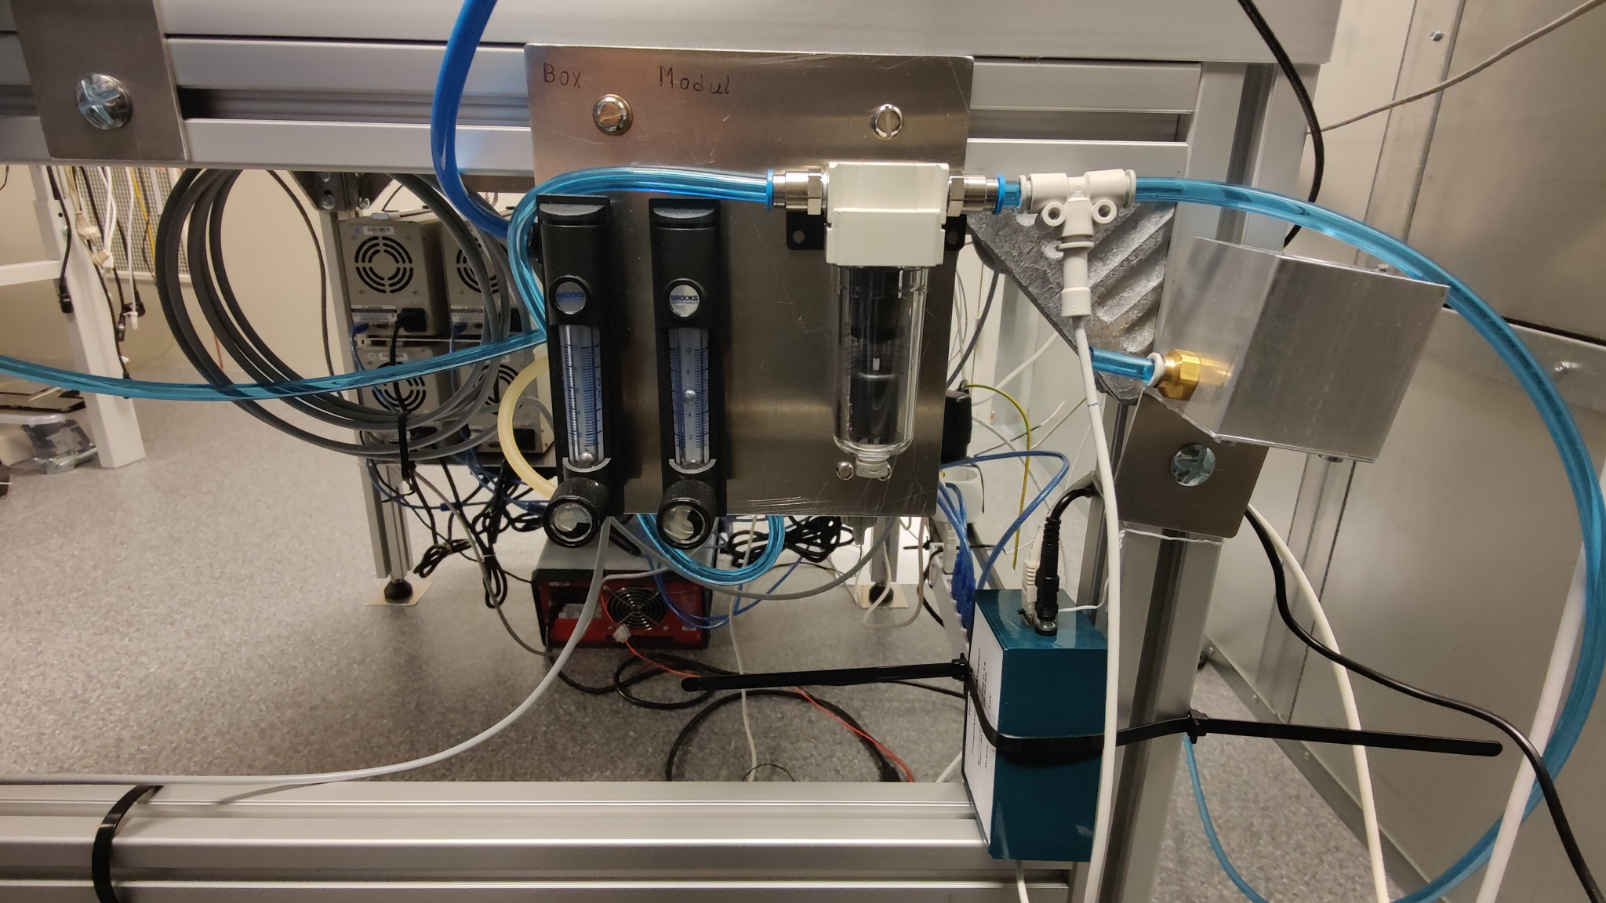
\includegraphics[width=7.5cm,height=10cm,keepaspectratio]{Figures/test/airflow-3.jpg}
        \caption{}\label{fig:airflow3}
    \end{subfigure}
    \caption{Picture of a) the airflow connectors, b) the Coldbox digital flowmeter, and c) flow control valves.}
    \label{fig:airflow}
\end{figure}

\newpage
\subsection{Electronics and connections}
\begin{figure}[h]
    \centering
    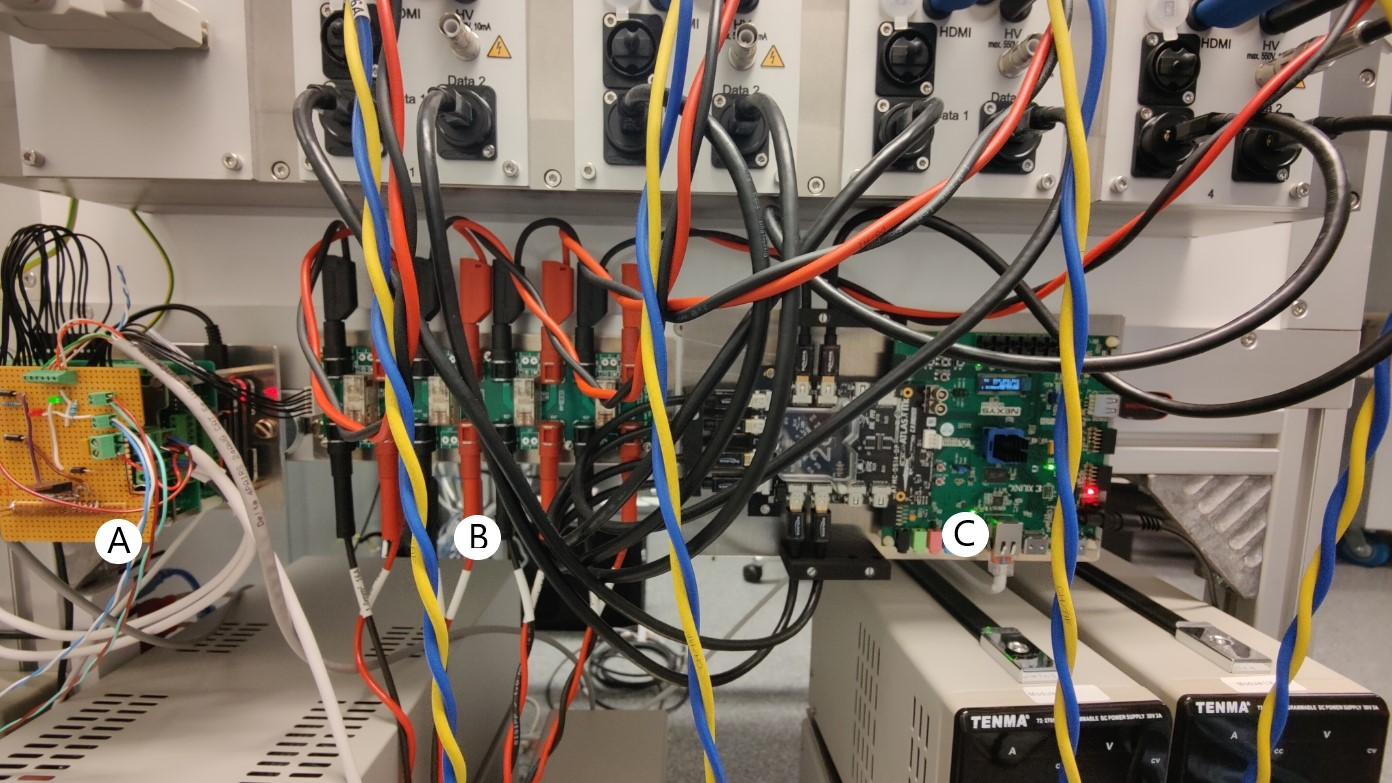
\includegraphics[width=10cm,height=11cm,keepaspectratio]{Figures/test/connections-5.jpg}
    \caption{An overview of the electronic and digital controllers and connections showing a) RPi (coldjiglib), b) Peltier switch and control board, and c) data ports}
    \label{fig:connections}
\end{figure}

\begin{figure}[h]
    
    \begin{subfigure}[b]{0.45\textwidth}
        \centering
        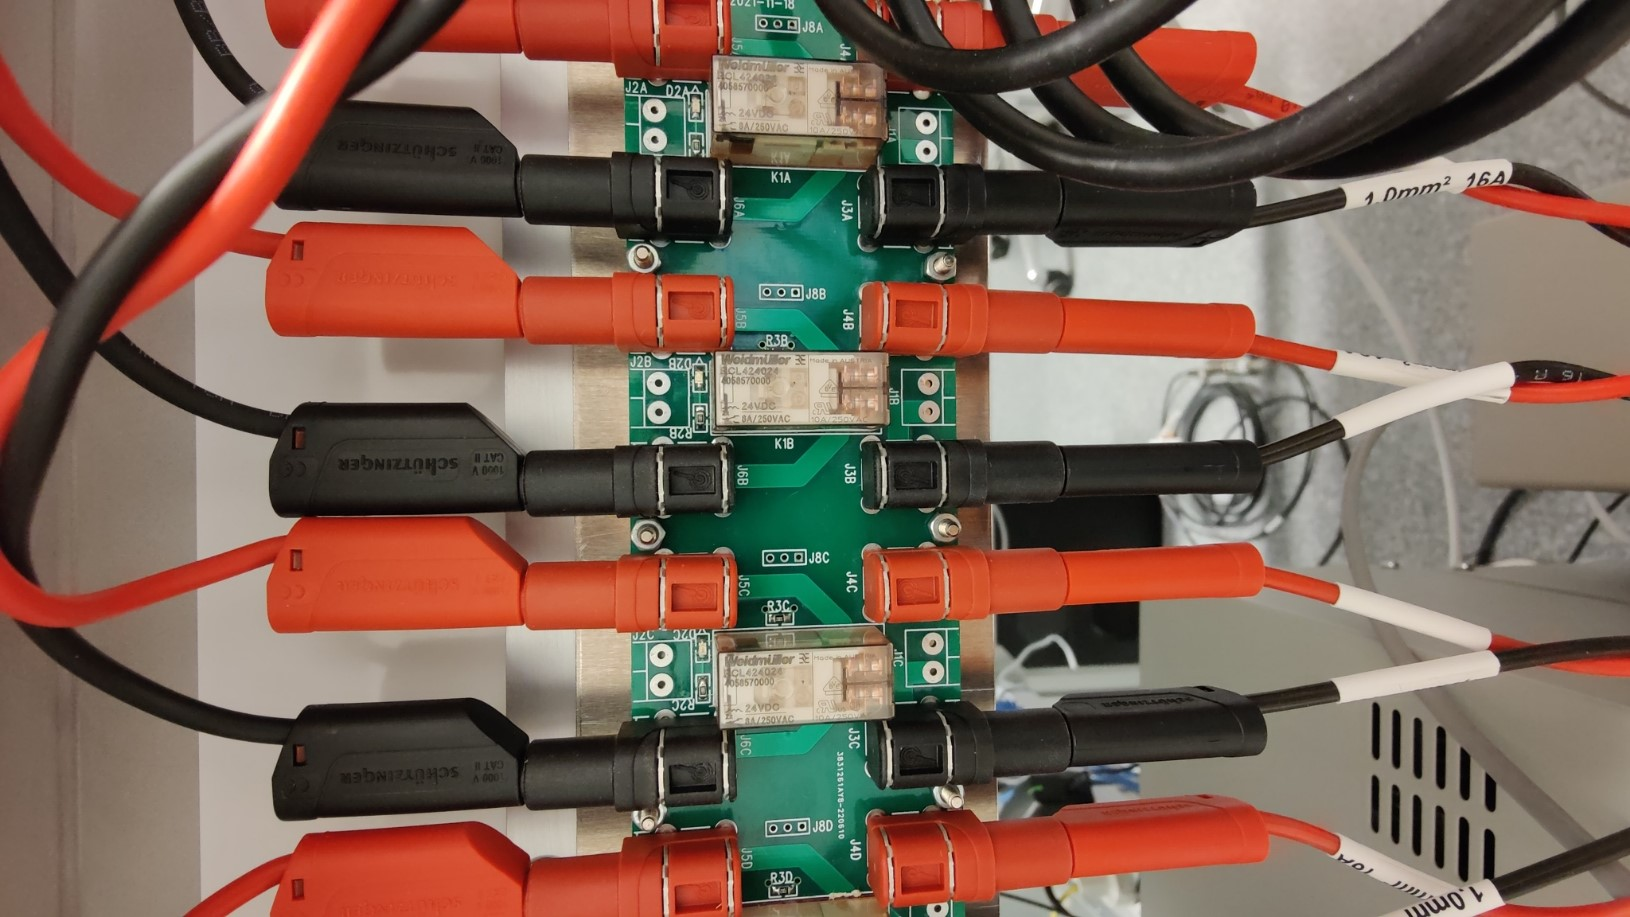
\includegraphics[width=7cm,height=10cm,keepaspectratio]{Figures/test/connections-3.jpg}
        \caption{}\label{fig:peltier1}
    \end{subfigure}
    ~
    \begin{subfigure}[b]{0.45\textwidth}
        \centering
        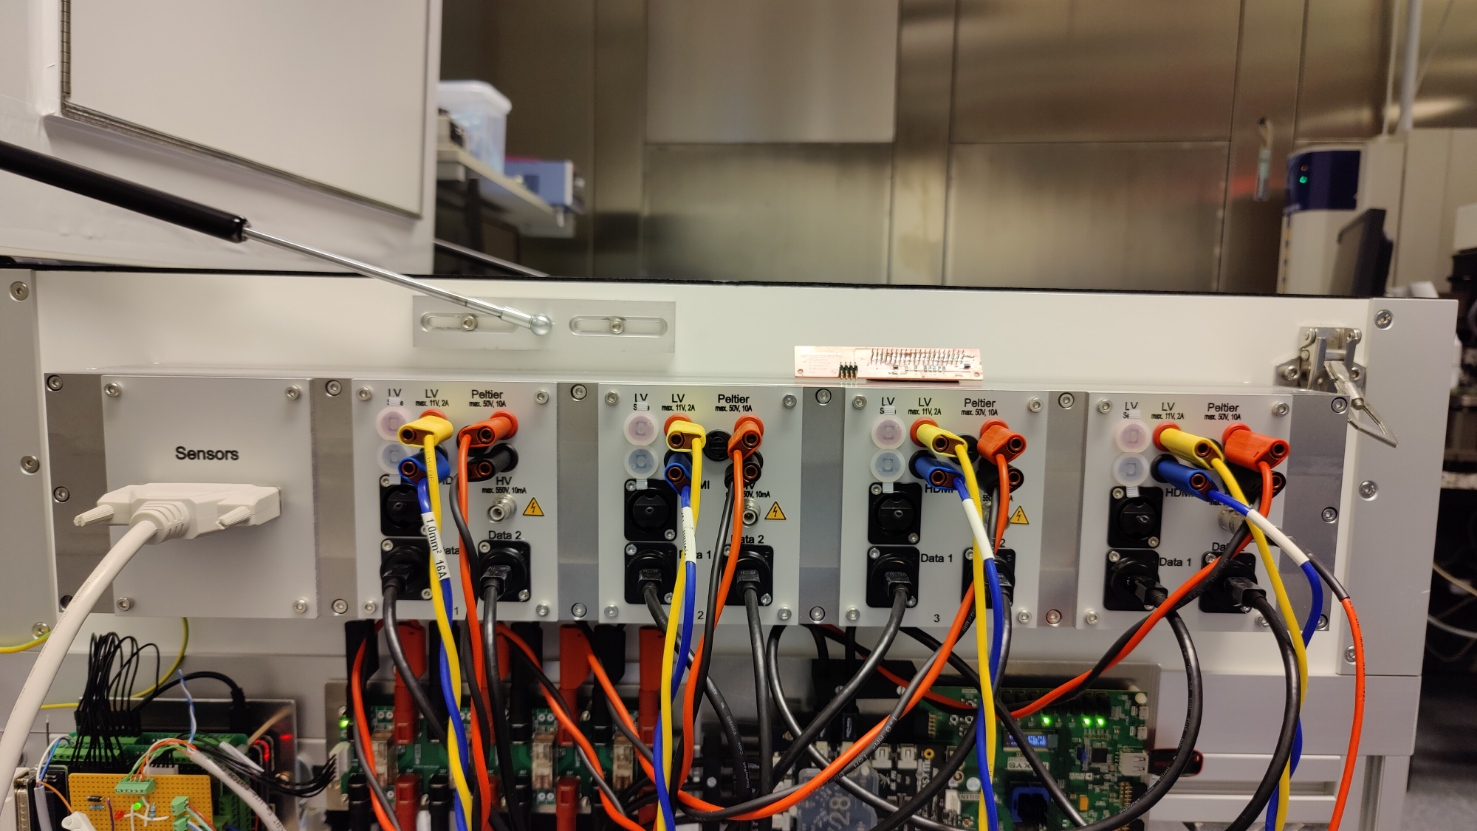
\includegraphics[width=7cm,height=10cm,keepaspectratio]{Figures/test/connections-6.jpg}
        \caption{}\label{fig:peltier2}
    \end{subfigure}

    \begin{subfigure}[b]{0.45\textwidth}
        \centering
        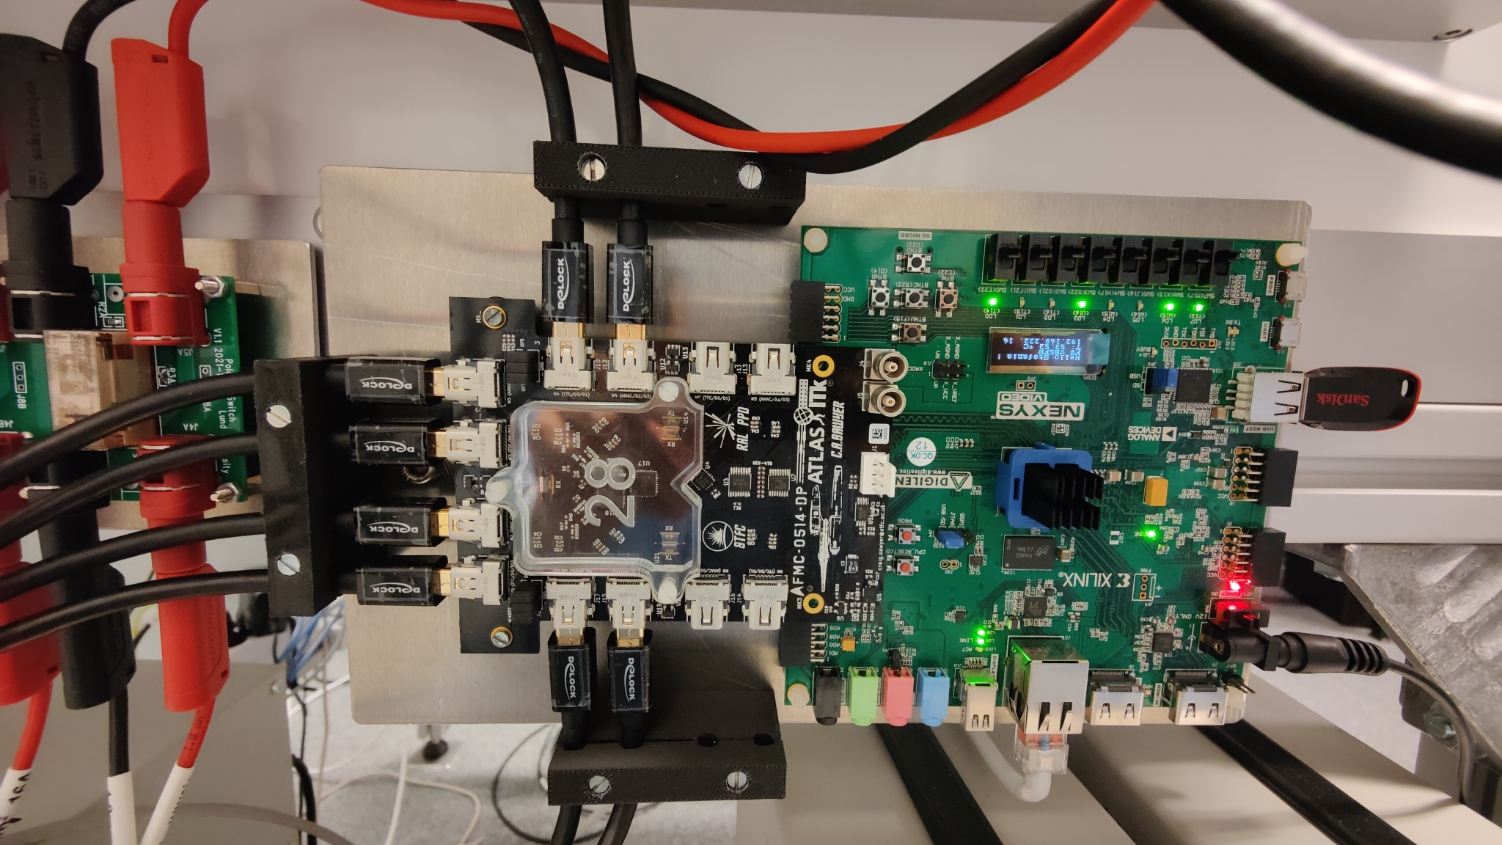
\includegraphics[width=7cm,height=10cm,keepaspectratio]{Figures/test/connections-4.jpg}
        \caption{}\label{fig:data}
    \end{subfigure}
    \caption{Picture of a) Peltier switchboard and controls, b) Peltier power connections, and c) data ports board}
    \label{fig:boards}
\end{figure}

\newpage
\subsection{Interlock}
\begin{figure}[h]
    \centering
    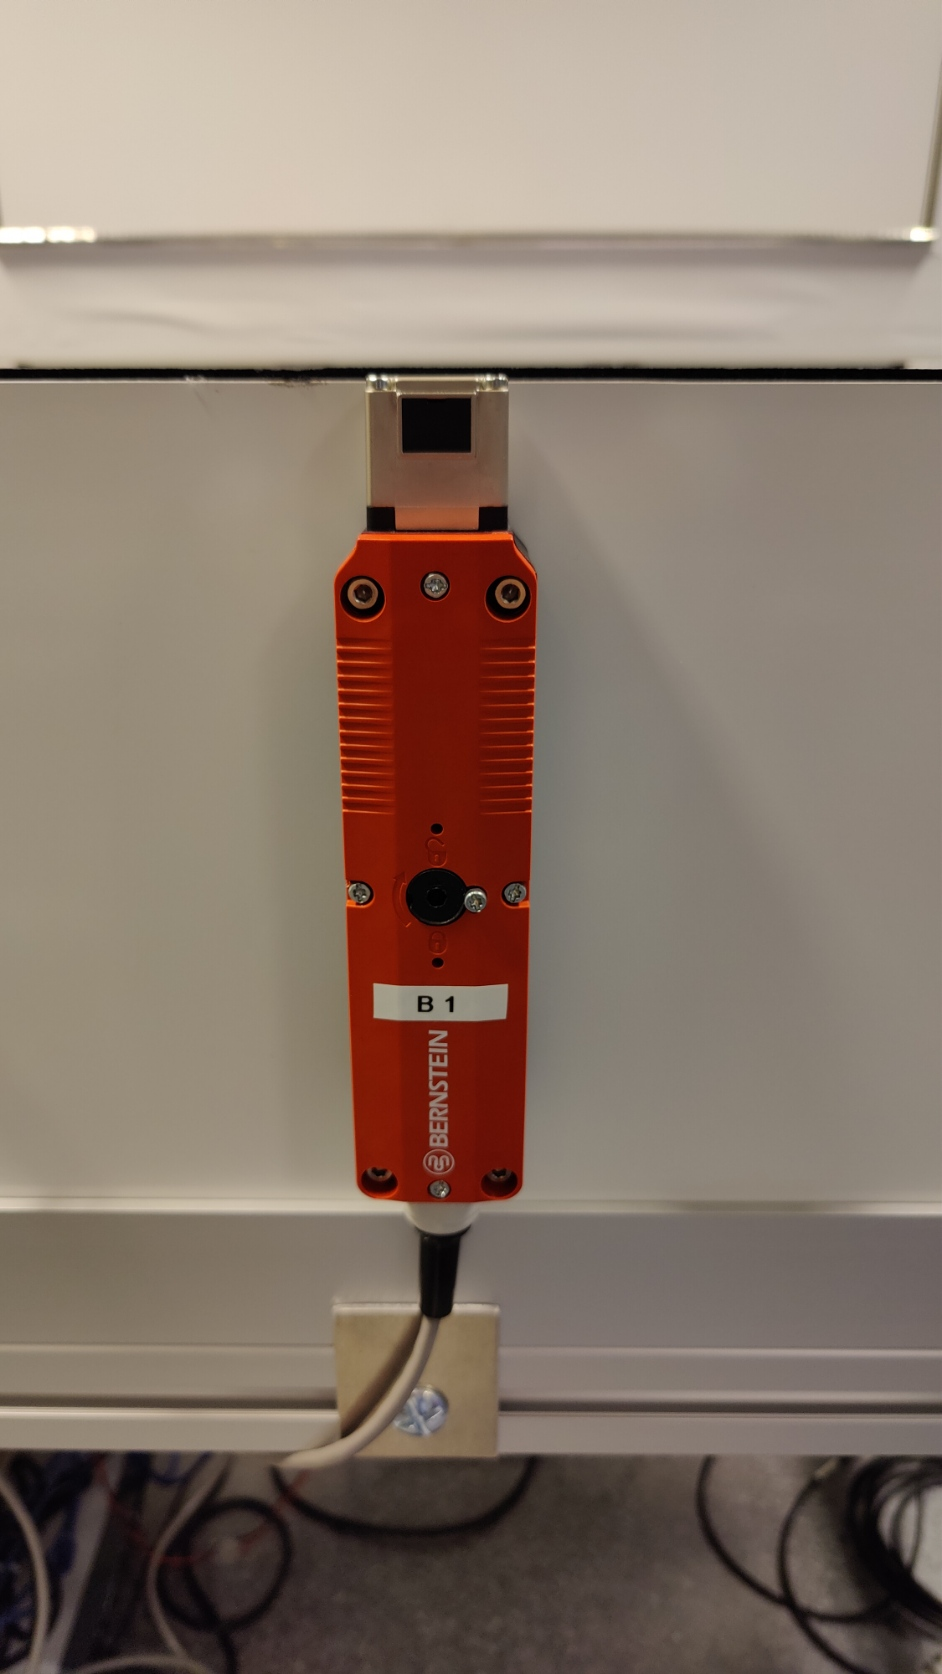
\includegraphics[width=10cm,height=11cm,keepaspectratio]{Figures/test/interlock.jpg}
    \caption{Picture of installed Interlock system on the Coldbox}
    \label{fig:interlock}
\end{figure}

\newpage
\subsection{Installation of modules}
\begin{figure}[h]    
    \begin{subfigure}[b]{0.4\textwidth}
        \centering
        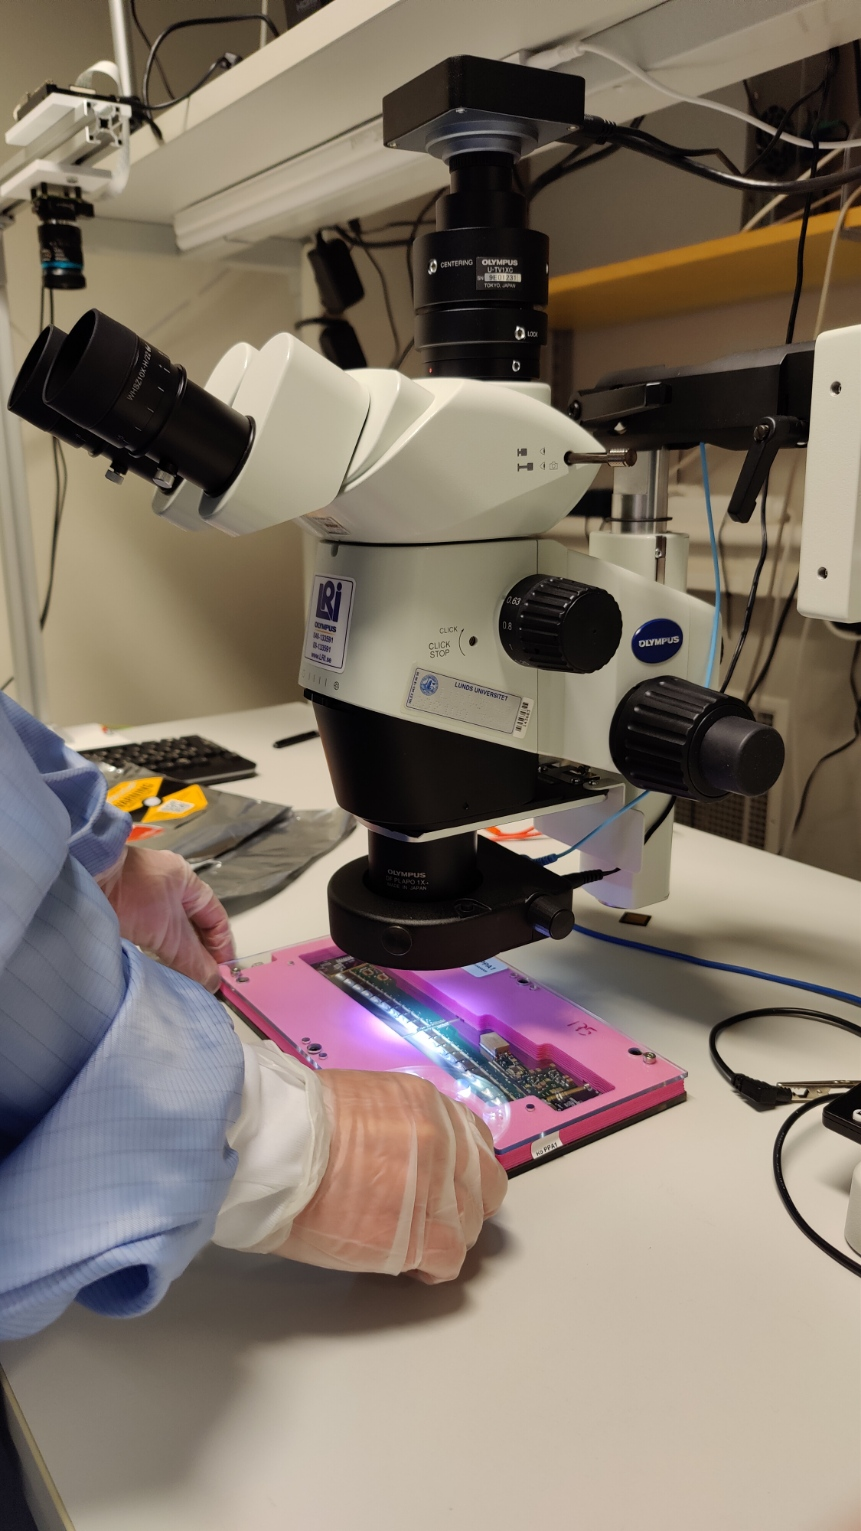
\includegraphics[width=7cm,height=8.5cm,keepaspectratio]{Figures/test/installation-4.jpg}
        \caption{}\label{fig:peltier1}
    \end{subfigure}
    ~
    \begin{subfigure}[b]{0.4\textwidth}
        \centering
        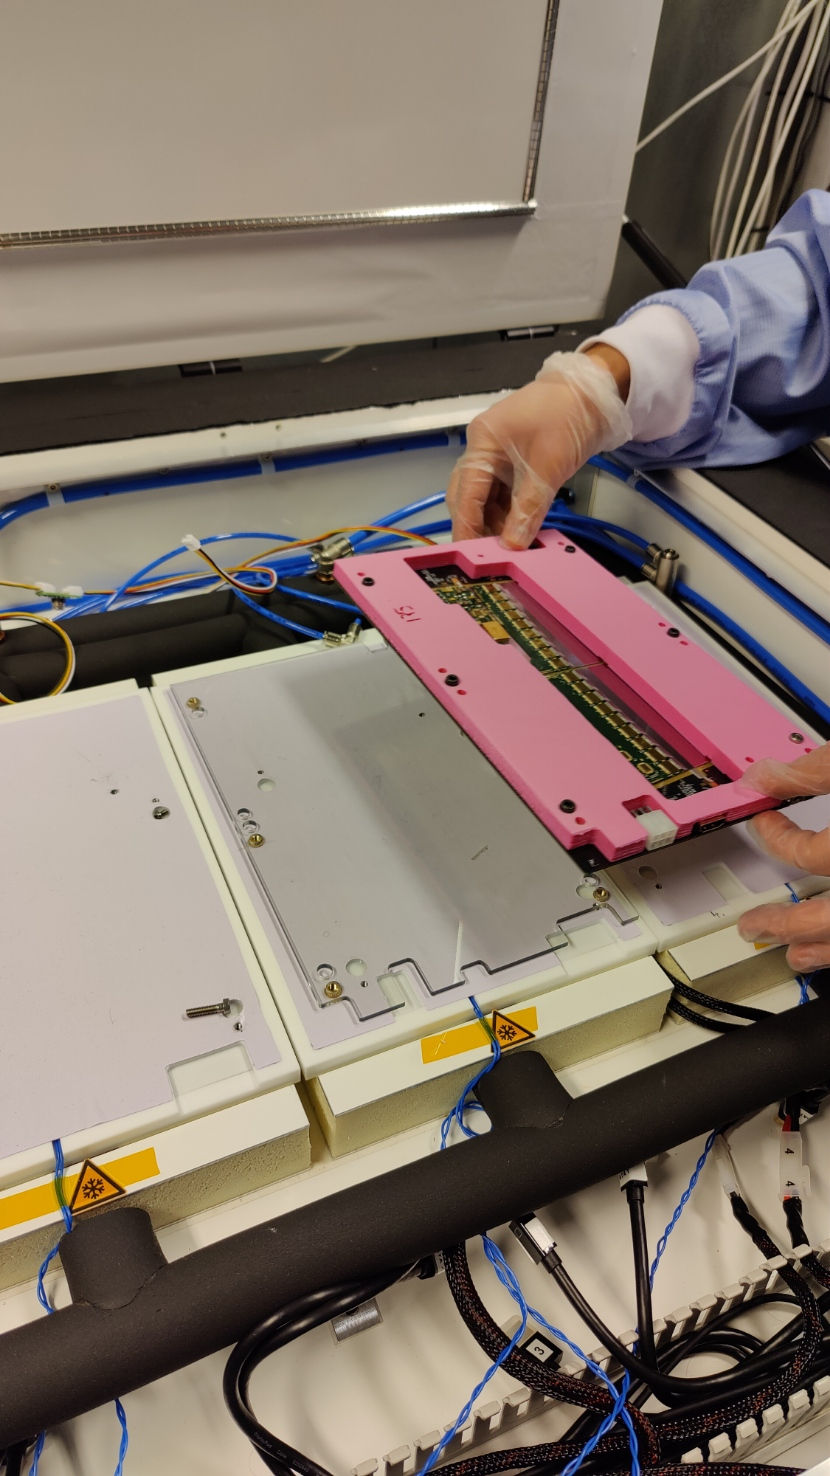
\includegraphics[width=7cm,height=8.5cm,keepaspectratio]{Figures/test/installation-2.jpg}
        \caption{}\label{fig:peltier2}
    \end{subfigure}

    \begin{subfigure}[b]{0.4\textwidth}
        \centering
        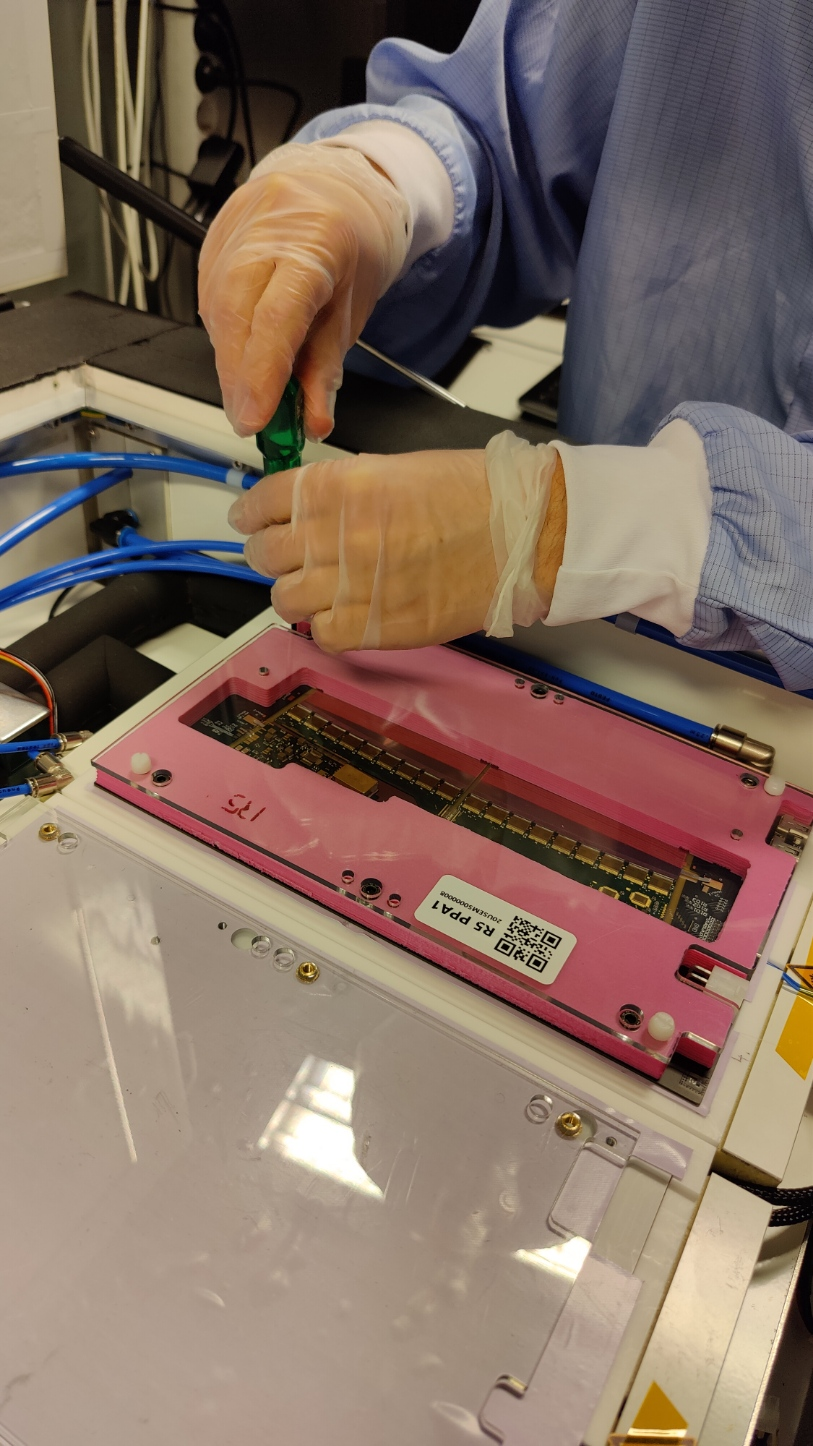
\includegraphics[width=7cm,height=8.5cm,keepaspectratio]{Figures/test/installation-1.jpg}
        \caption{}\label{fig:data}
    \end{subfigure}
    \caption{Inspection and installation of modules to the Coldbox}
    \label{fig:installation}
\end{figure}

\newpage
\section{Large format of Results' plots}

\begin{sidewaysfigure}[h]
    \centering
    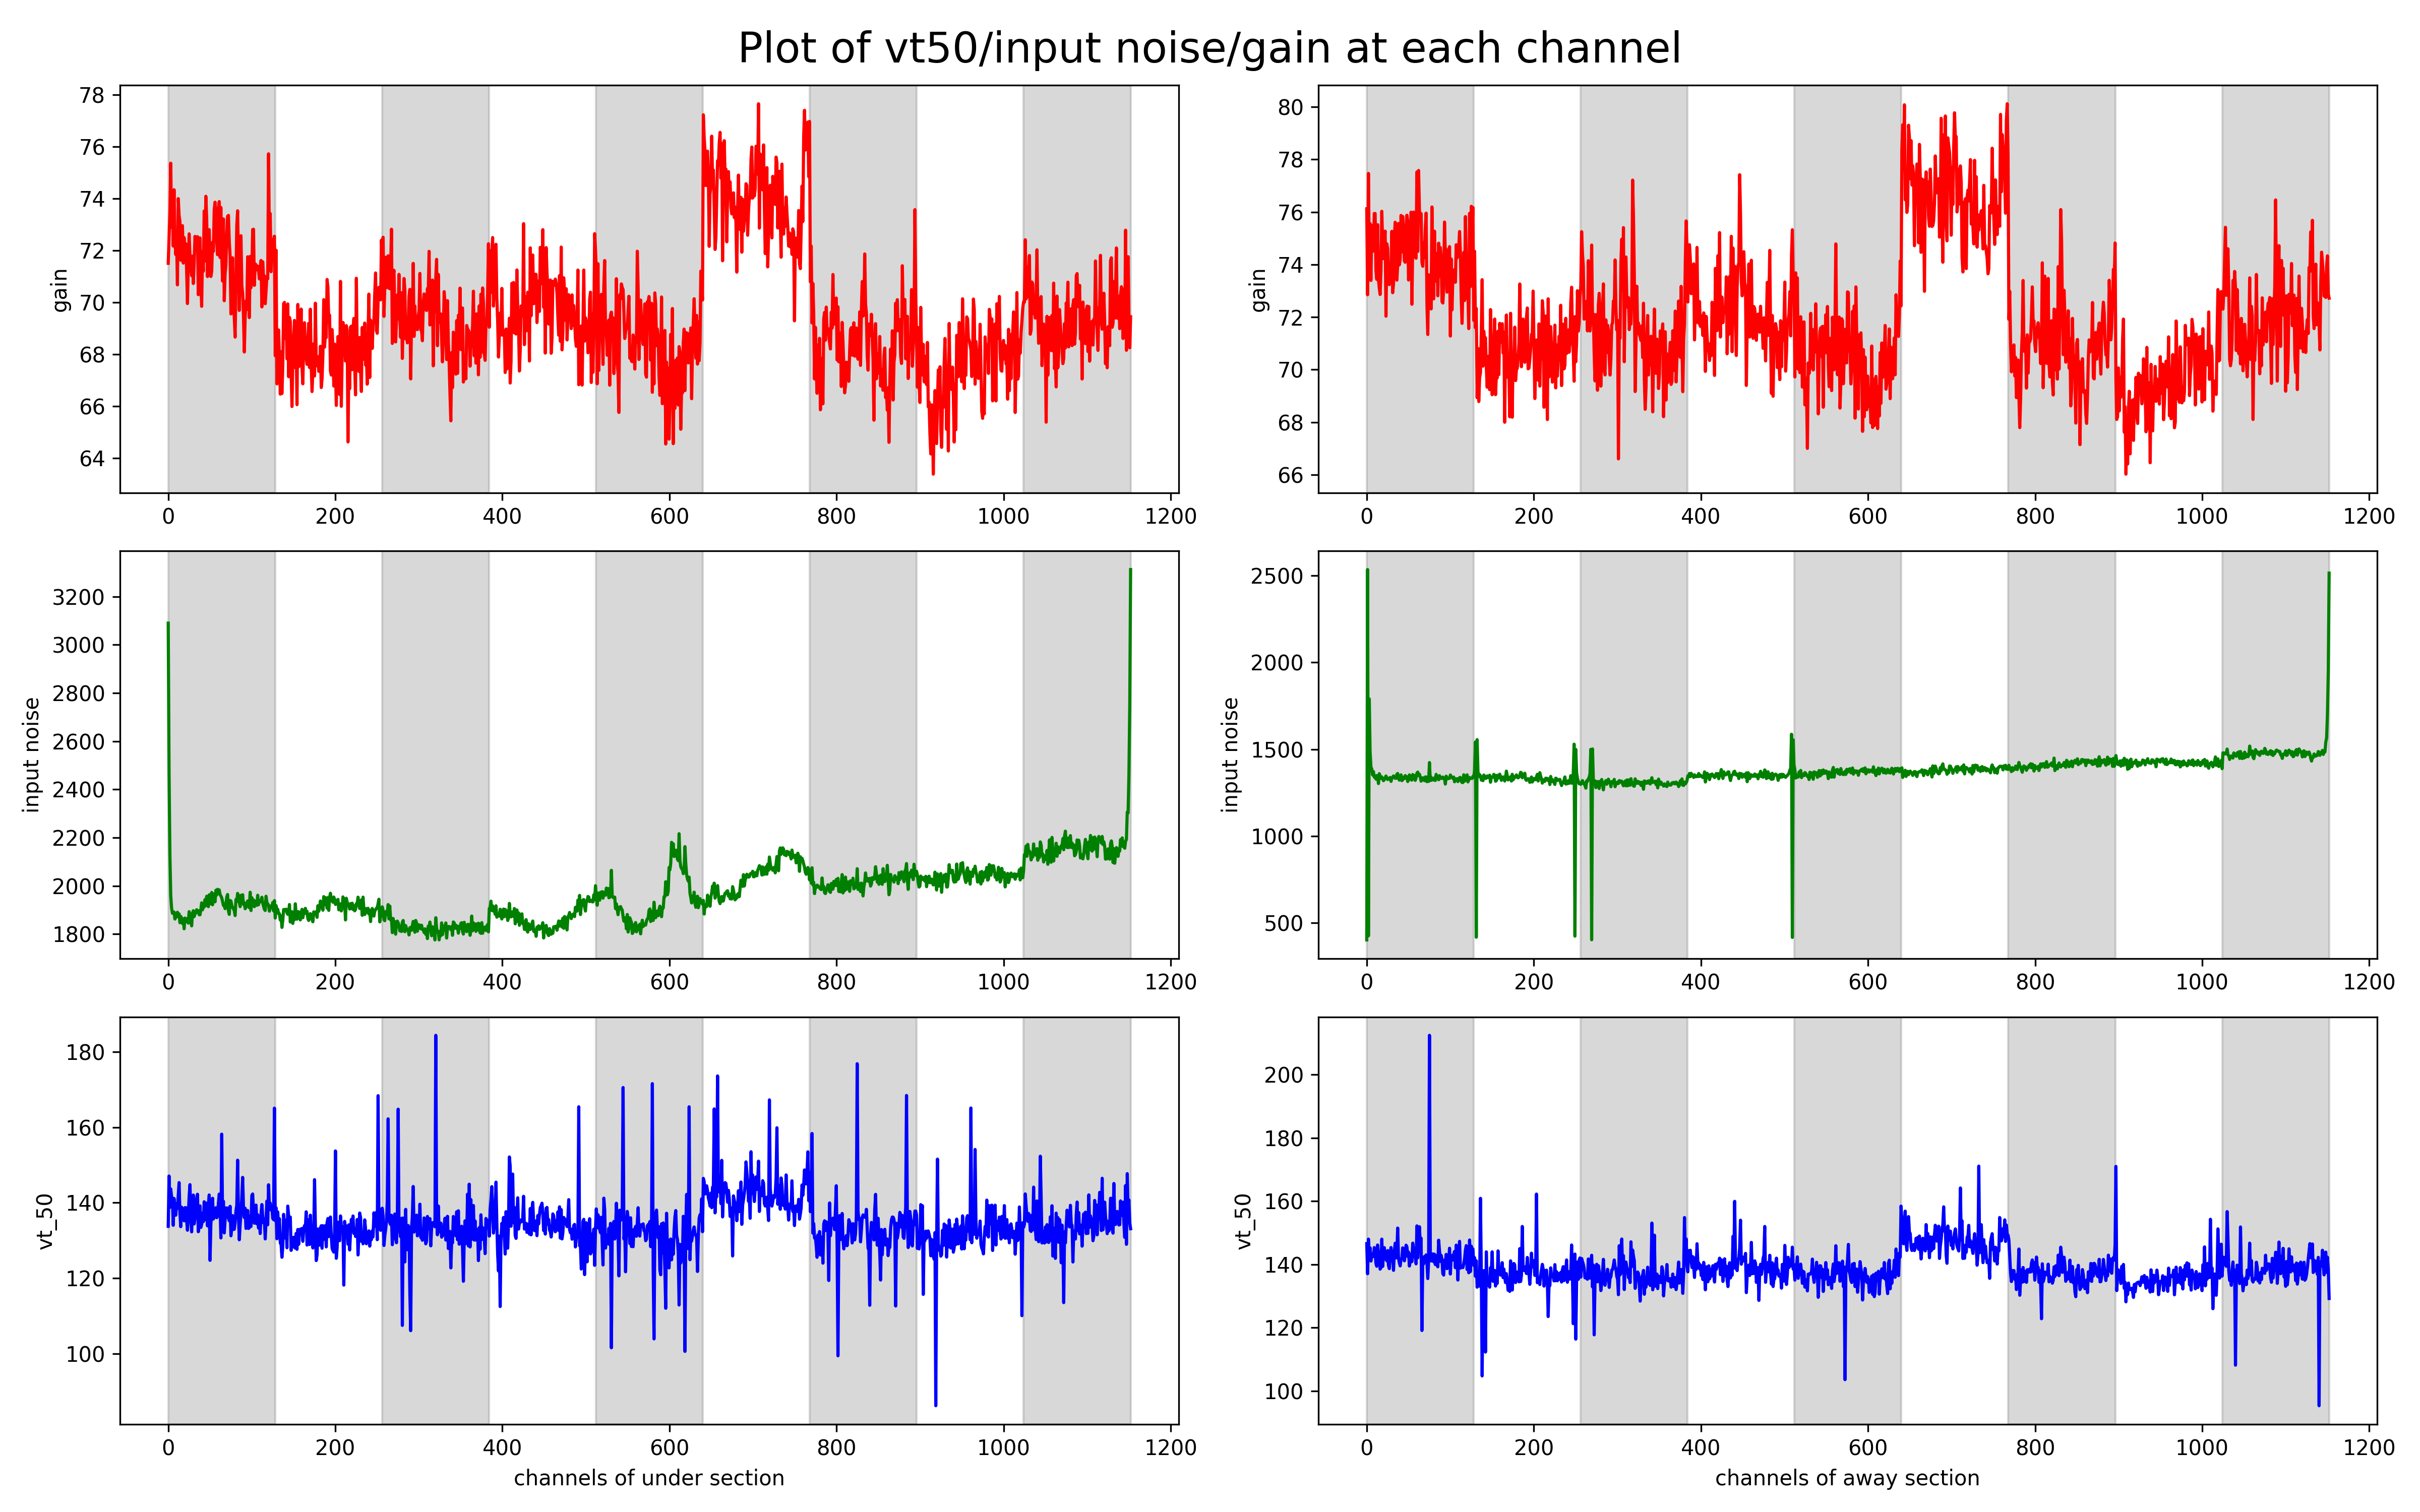
\includegraphics[width=25cm,height=20cm,keepaspectratio]{Figures/results/LTRT_1_plot.png}
    \caption{Plots of $3$ performed electrical test by ABCstar full test during the "LTRT COLD TEST 1" stage, showing the result of VT$50$, input noise, and gain for two hybrids (under and above) of a Pre Production A (PPA) R5 module.}
    \label{fig:LTRT_result_1_large}
\end{sidewaysfigure}

\begin{sidewaysfigure}[h]
    \centering
    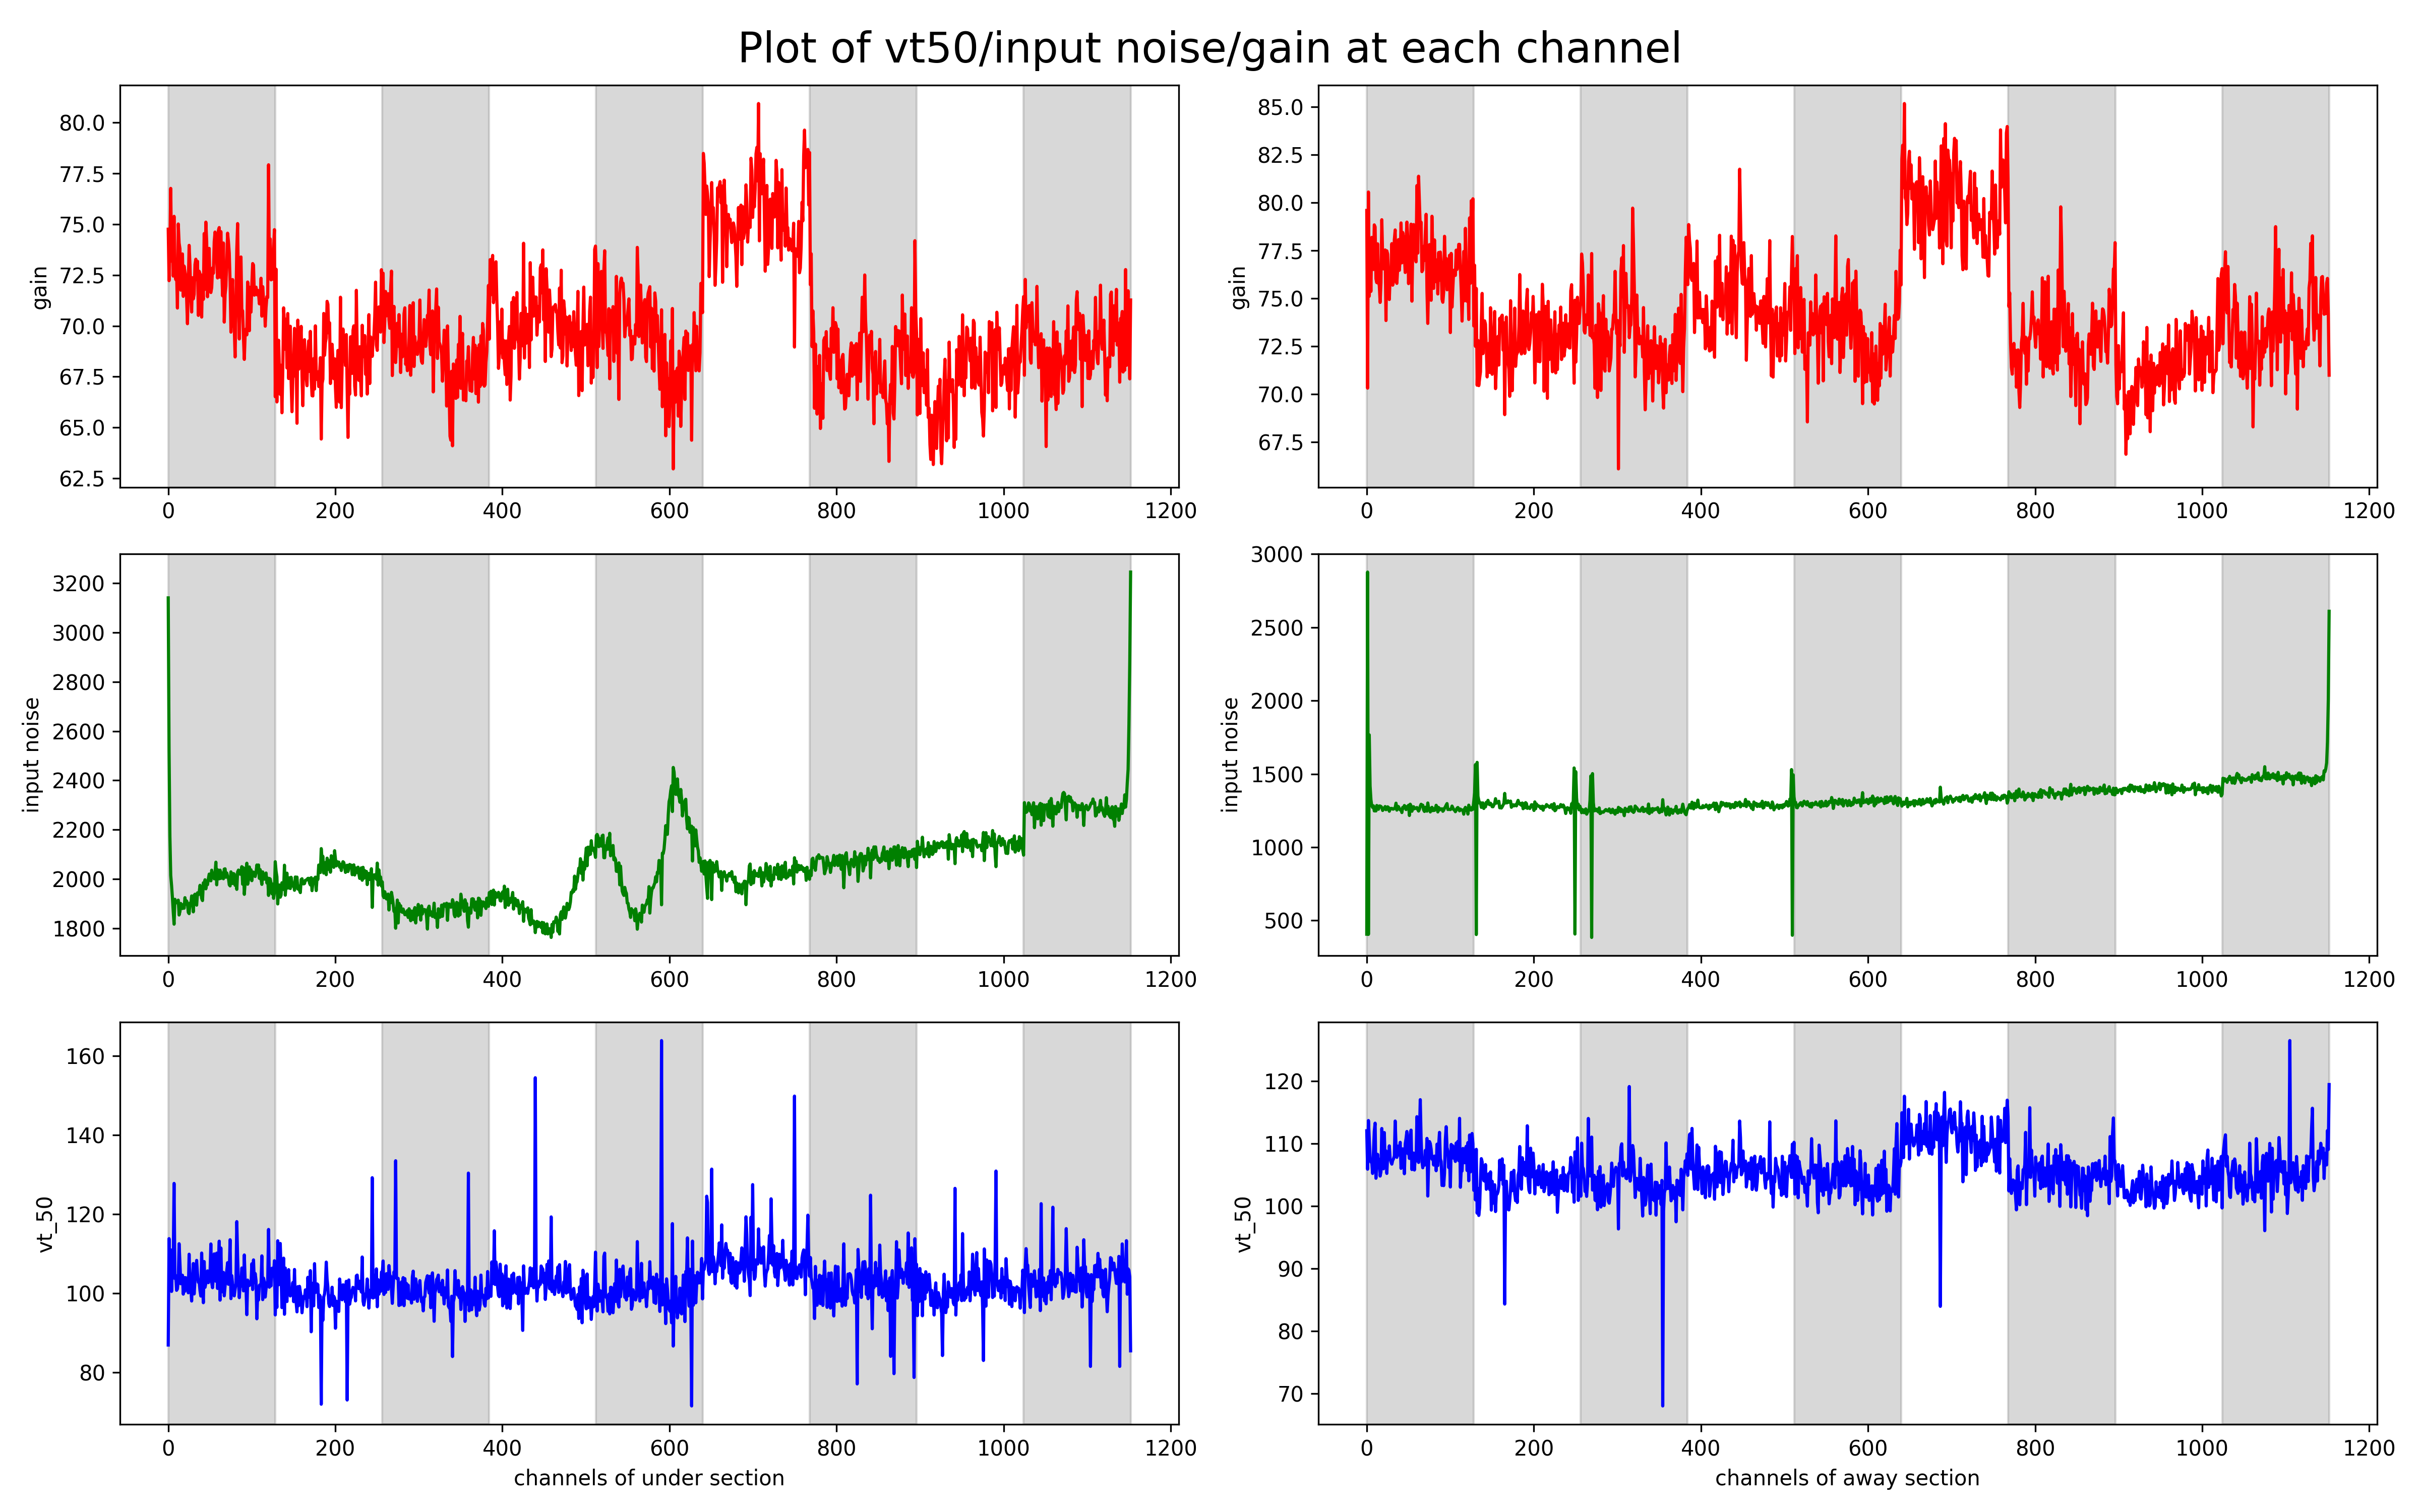
\includegraphics[width=25cm,height=20cm,keepaspectratio]{Figures/results/LTRT_2_plot.png}
    \caption{Plots of $3$ performed electrical test by ABCstar full test during the "LTRT COLD TEST 2" stage, showing the result of VT$50$, input noise, and gain for two hybrids (under and above) of a Pre Production A (PPA) R5 module.}
    \label{fig:LTRT_result_2_large}
\end{sidewaysfigure}

\begin{sidewaysfigure}[h]
    \centering
    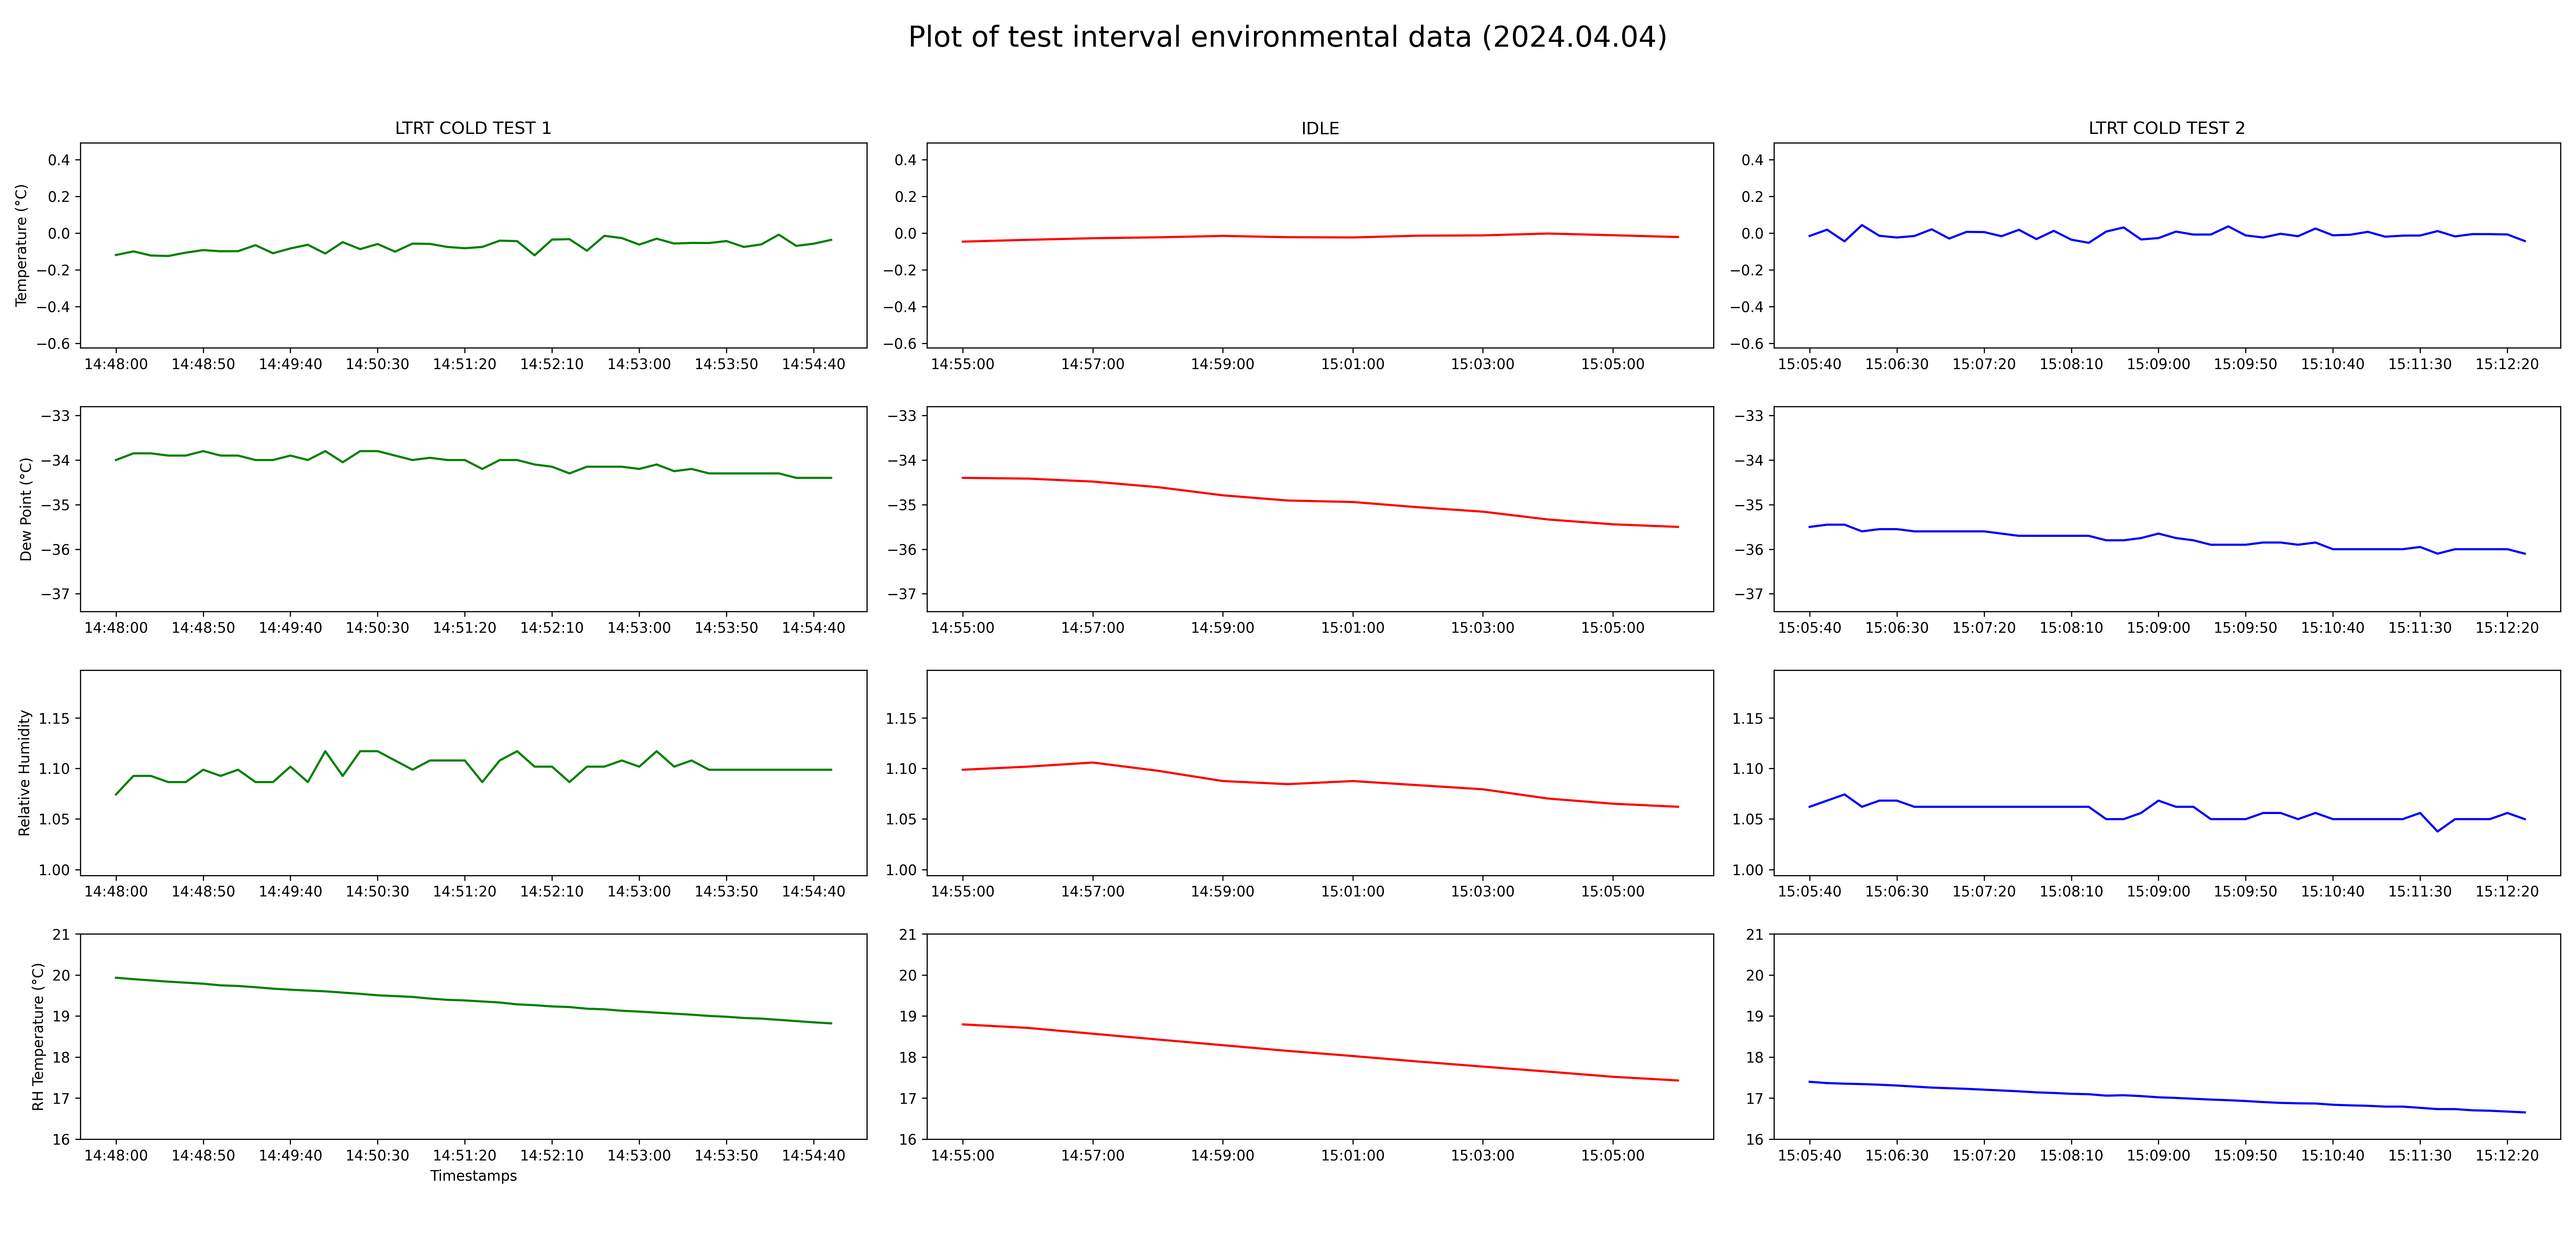
\includegraphics[width=25cm,height=20cm,keepaspectratio]{Figures/results/env_plot_20240404_.png}
    \caption{Plots environmental data during the time span of the LTRT test shown in Fig.\ref{fig:LTRT_result_1_large} including the data for Temperature, Dew point, Relative humidity, and Relative humidity temperature.}
    \label{fig:env_1_large}
\end{sidewaysfigure}

\begin{sidewaysfigure}[h]
    \centering
    \includegraphics[width=25cm,height=20cm,keepaspectratio]{Figures/results/amac_plot_20240404_.png}
    \caption{Plots AMAC electrical data during the time span of the LTRT test shown in Fig.\ref{fig:LTRT_result_1_large} including the data for input and output currents and voltage.}
    \label{fig:amac_1_large}
\end{sidewaysfigure}
\chapter{Appendix B: Additional tables} % Main appendix title

\label{AppendixB} % Change X to a consecutive letter; for referencing this appendix elsewhere, use \ref{AppendixX}

%More tables of information
\begin{comment}
\section{TestType Structure for STAR Hybrid Assembly}
\label{sec:teststructure}


\begin{table}[H]
    \centering
    \begin{tabular}{|c|c|c|c|c|}
        \hline
        Name                   & Description & dataType & valueType & Required \\ \hline
        enc\_est\_away         & -           & array    & float     & True     \\ \hline
        enc\_est\_under        & -           & array    & float     & True     \\ \hline
        occupancy\_mean\_away  & -           & array    & float     & True     \\ \hline
        occupancy\_mean\_under & -           & array    & float     & True     \\ \hline
        occupancy\_rms\_away   & -           & array    & float     & True     \\ \hline
        occupancy\_rms\_under  & -           & array    & float     & True     \\ \hline
        offset\_away           & -           & array    & float     & True     \\ \hline
        offset\_under          & -           & array    & float     & True     \\ \hline
    \end{tabular}
    \caption{Table of parameters of the Noise Occupancy test (NO\_PPA)}
\end{table}


\begin{table}[H]
    \centering
    \begin{tabular}{|c|c|c|c|c|}
        \hline 
        Name        & Description & dataType & valueType & Required \\ \hline \hline
        trim\_away  & -           & array    & float     & True     \\ \hline
        trim\_under & -           & array    & float     & True     \\ \hline
    \end{tabular}
    \caption{Table of parameters of the Pedestal Trim test (PEDESTAL\_TRIM\_PPA)}
\end{table}


\begin{table}[H]
    \centering
        \begin{tabular}{|c|c|c|c|c|}
        \hline 
        Name               & Description & dataType & valueType & Required \\ \hline \hline
        StrobeDelay\_away  & -           & array    & float     & True     \\ \hline
        StrobeDelay\_under & -           & array    & float     & True     \\ \hline
    \end{tabular}
    \caption{Table of parameters of the Strobe Delay test (STROBE\_DELAY\_PPA)}
\end{table}


\begin{table}[H]
    \centering
    \begin{tabular}{|c|c|c|c|c|}
        \hline 
        Name                & Description & dataType & valueType & Required \\ \hline \hline
        gain away           & -           & array    & float     & True     \\ \hline
        gain mean away      & -           & array    & float     & True     \\ \hline
        gain\_mean\_under   & -           & array    & float     & True     \\ \hline
        gain\_rms\_away     & -           & array    & float     & True     \\ \hline
        gain\_rms\_under    & -           & array    & float     & True     \\ \hline
        gain\_under         & -           & array    & float     & True     \\ \hline
        innse\_away         & -           & array    & float     & True     \\ \hline
        innse\_mean\_away   & -           & array    & float     & True     \\ \hline
        innse\_mean\_under  & -           & array    & float     & True     \\ \hline
        innse\_rms\_away    & -           & array    & float     & True     \\ \hline
        innse\_rms\_under   & -           & array    & float     & True     \\ \hline
        innse\_under        & -           & array    & float     & True     \\ \hline
        offset\_mean\_away  & -           & array    & float     & True     \\ \hline
        offset\_mean\_under & -           & array    & float     & True     \\ \hline
        offset\_rms\_away   & -           & array    & float     & True     \\ \hline
        offset\_rms\_under  & -           & array    & float     & True     \\ \hline
        outnse\_away        & -           & array    & float     & True     \\ \hline
        outnse\_under       & -           & array    & float     & True     \\ \hline
        rc\_fit\_away       & -           & array    & float     & True     \\ \hline
        rc\_fit\_under      & -           & array    & float     & True     \\ \hline
        vt50\_away          & -           & array    & float     & True     \\ \hline
        vt50\_mean\_away    & -           & array    & float     & True     \\ \hline
        vt50\_mean\_under   & -           & array    & float     & True     \\ \hline
        vt50\_rms\_away     & -           & array    & float     & True     \\ \hline
        vt50\_rms\_under    & -           & array    & float     & True     \\ \hline
        vt50\_under         & -           & array    & float     & True     \\ \hline
    \end{tabular}
    \caption{Table of parameters of the Responce Curve test (RESPONSE\_CURVE\_PPA)}
\end{table}


\end{comment}
%\include{Appendices/AppendixC}

%----------------------------------------------------------------------------------------
%	ABBREVIATIONS
%----------------------------------------------------------------------------------------

\begin{abbreviations}{ll} % Include a list of abbreviations (a table of two columns)

\textbf{HEP} & \textbf{H}igh \textbf{E}nergy \textbf{P}hysics\\
\textbf{ATLAS} & \textbf{A} \textbf{T}oroidal \textbf{L}HC \textbf{A}pparatu\textbf{S}\\
\textbf{Cern} & \textbf{C}onseil \textbf{E}uropéen pour la \textbf{R}echerche \textbf{N}ucléaire\\
\textbf{LHC} & \textbf{L}arge \textbf{H}adron \textbf{C}olider\\
\textbf{HL-LHC} &  \textbf{H}igh-\textbf{L}uminosity \textbf{L}arge \textbf{H}adron \textbf{C}olider\\
\textbf{TeV} & \textbf{T}era \textbf{e}lectron\textbf{V}olts\\
\textbf{SCT} & \textbf{S}emi\textbf{C}onductor \textbf{T}racker\\
\textbf{TRT} & \textbf{T}ransition \textbf{R}adiation \textbf{T}racker\\
\textbf{LTRT} & \textbf{L}ong \textbf{T}erm \textbf{R}eliability \textbf{T}est\\
\textbf{ITSDAQ} & \textbf{IT}k \textbf{S}trips \textbf{D}ata \textbf{A}c\textbf{Q}uisition\\
\textbf{ABC}star & \textbf{A}tlas \textbf{B}inary \textbf{C}hip  \\
\textbf{HCC}star & \textbf{H}ybrid \textbf{C}ontrol \textbf{C}hip  \\
\textbf{PCB} & \textbf{P}rinted \textbf{C}ircuit \textbf{B}oard \\
\textbf{AMAC} & \textbf{A}utonomous  \textbf{M}onitoring \textbf{A}nd \textbf{C}ontrol \\
\textbf{innse} & \textbf{in}put \textbf{n}oi\textbf{se} \\
\textbf{outnse} & \textbf{out}put \textbf{n}oi\textbf{se} \\
\textbf{LV} & \textbf{L}wo \textbf{V}oltage \\
\textbf{HV} & \textbf{H}igh \textbf{V}oltage \\
\textbf{DP} & \textbf{D}ew \textbf{P}oint \\
\textbf{RH} & \textbf{R}elative \textbf{H}umidity \\


%\textbf{LAr} & \textbf{L}iquid \textbf{Ar}gon\\


\end{abbreviations}

%----------------------------------------------------------------------------------------
%	PHYSICAL CONSTANTS/OTHER DEFINITIONS
%----------------------------------------------------------------------------------------
\begin{comment}

\begin{constants}{lr@{${}={}$}l} % The list of physical constants is a three column table

% The \SI{}{} command is provided by the siunitx package, see its documentation for instructions on how to use it

Speed of Light & $c_{0}$ & \SI{2.99792458e8}{\meter\per\second} (exact)\\
%Constant Name & $Symbol$ & $Constant Value$ with units\\

\end{constants}

\end{comment}


%----------------------------------------------------------------------------------------
%	SYMBOLS
%----------------------------------------------------------------------------------------
\begin{comment}
\begin{symbols}{lll} % Include a list of Symbols (a three column table)

$a$ & distance & \si{\meter} \\
$P$ & power & \si{\watt} (\si{\joule\per\second}) \\
%Symbol & Name & Unit \\

\addlinespace % Gap to separate the Roman symbols from the Greek

$\omega$ & angular frequency & \si{\radian} \\

\end{symbols}
\end{comment}


%----------------------------------------------------------------------------------------
%	BIBLIOGRAPHY
%----------------------------------------------------------------------------------------

\printbibliography[heading=bibintoc]

%----------------------------------------------------------------------------------------

\end{document}  
